\chapter{การวิเคราะห์การถดถอย}

การวิเคราะห์การถดถอย (Regression Analysis) ถือเป็นรากฐานสำคัญทางสถิติและเป็นองค์ประกอบหลักของการเรียนรู้แบบมีผู้สอน (Supervised Learning) ในเทคนิคการเรียนรู้ของเครื่อง (Machine Learning) โดยมีเป้าหมายเพื่อสร้างตัวแบบทางคณิตศาสตร์ที่อธิบายความสัมพันธ์และทำนายค่าของตัวแปรตาม (Dependent Variable) จากตัวแปรอิสระ (Independent Variables) หรือคุณลักษณะ (Features) ที่กำหนดให้

เนื้อหาในบทนี้จะนำเสนอหลักการและระเบียบวิธีของการวิเคราะห์การถดถอยอย่างเป็นลำดับขั้นตอน เริ่มต้นจาก \textbf{ความรู้เบื้องต้นเกี่ยวกับการถดถอย} เพื่อเรียนรู้พื้นฐานแนวคิดที่สำคัญ จากนั้นจะลงในรายละเอียดของ \textbf{การถดถอยเชิงเส้นอย่างง่าย (Simple Linear Regression)} และ \textbf{การถดถอยเชิงเส้นพหุคูณ (Multiple Linear Regression)} ซึ่งเป็นเครื่องมือพื้นฐานในการวิเคราะห์ความสัมพันธ์เชิงเส้น และส่วนสุดท้ายจะกล่าวถึง \textbf{การถดถอยโลจิสติค (Logistic Regression)} ซึ่งเป็นการขยายแนวคิดไปสู่การจัดการกับปัญหาการจำแนกประเภท (Classification) สำหรับข้อมูลเชิงคุณภาพ อันเป็นเทคนิคที่มีความสำคัญอย่างยิ่งในการประยุกต์ใช้งานจริง ... Not compltete...

%####################################
\section{ความรู้เบื้องต้นเกี่ยวกับการถดถอย}

พื้นฐานความเข้าใจเกี่ยวกับการวิเคราะห์การถดถอย (Regression Analysis) โดยครอบคลุม 3 หัวข้อหลัก ได้แก่ \textbf{แนวคิดการถดถอย} ซึ่งอธิบายกลไกการทำงานในการหาความสัมพันธ์ระหว่างตัวแปร \textbf{ความแตกต่างระหว่างการถดถอยและการจำแนกประเภท} เพื่อจำแนกประเภทของปัญหาการเรียนรู้ตามลักษณะของข้อมูล และ \textbf{การประยุกต์การวิเคราะห์การถดถอย} ที่แสดงให้เห็นถึงบทบาทและความสำคัญของเครื่องมือนี้ในบริบทของงานจริงหลากหลายสาขา

\subsection{หลักการและแนวคิดการถดถอย}

ในมุมมองของการเรียนรู้ของเครื่อง (Machine Learning) การถดถอย (Regression) จัดเป็นรากฐานสำคัญของการเรียนรู้แบบมีผู้สอน (Supervised Learning) โดยมีวัตถุประสงค์หลักเพื่อสร้างตัวแบบทางคณิตศาสตร์สำหรับทำนายค่าของตัวแปรเป้าหมาย (Target Variable) หรือตัวแปรตาม (Dependent Variable) ที่มีลักษณะเป็นข้อมูลต่อเนื่อง (Continuous Data) โดยอาศัยความสัมพันธ์กับตัวแปรนำเข้า (Input Features) หรือตัวแปรอิสระ (Independent Variables) 1 ตัวหรือมากกว่า 1 ตัวขึ้นไป

\begin{myBox}[]{หลักการพื้นฐานการวิเคราะห์การถดถอย}{}
หลักการพื้นฐานคือ การค้นหาฟังก์ชัน $f(\mathbf{x})$ ที่สามารถอธิบายความสัมพันธ์ระหว่างตัวแปรอิสระ $\mathbf{x}$ และตัวแปรตาม $Y$ ได้อย่างแม่นยำที่สุด โดยทั่วไปสามารถเขียนแทนด้วยสมการ:

$$Y = f(\mathbf{x}; \boldsymbol{\theta}) + \epsilon$$

\noindent โดยที่ 

$\boldsymbol{\beta}$ แทน ชุดพารามิเตอร์ของตัวแบบที่ต้องได้รับการปรับแต่ง (Optimize) ผ่านการฝึกฝน (Training) 

$\epsilon$ แทน ค่าความคลาดเคลื่อน (Error Term) ที่ไม่สามารถอธิบายได้ด้วยตัวแบบ 


\noindent
เป้าหมายของการเรียนรู้คือ การหาค่า $\boldsymbol{\beta}$ ที่ทำให้ค่าความสูญเสีย (Loss Function) ซึ่งวัดความแตกต่างระหว่างค่าทำนาย $\hat{y}$ และค่าจริง $Y$ มีค่าน้อยที่สุด
\end{myBox}
	
ตัวอย่างของการประยุกต์ใช้การถดถอย ได้แก่ การทำนายราคาอสังหาริมทรัพย์จากคุณลักษณะของบ้าน การพยากรณ์อุณหภูมิรายวัน การคาดการณ์ยอดขายสินค้าตามงบประมาณทางการตลาด รวมไปถึงการประยุกต์ใช้ทางการแพทย์ เช่น การทำนายระดับคอเลสเตอรอลในเลือดโดยพิจารณาจากปัจจัยเสี่ยงต่าง ๆ (อายุ น้ำหนัก และพฤติกรรมการออกกำลังกาย) หรือการพยากรณ์ระยะเวลาการฟื้นตัวของผู้ป่วยหลังการผ่าตัด** ซึ่งหัวใจสำคัญคือผลลัพธ์ที่ได้จะเป็นค่าตัวเลขที่มีความต่อเนื่อง ไม่ใช่เพียงการระบุหมวดหมู่เหมือนในการจำแนกประเภท

\subsection{ประเภทปัญหาการถดถอย}
ในทางปฏิบัติปัญหาการถดถอยสามารถจำแนกประเภทได้โดยพิจารณาจากจำนวนของตัวแปรอิสระ (Independent Variables) หรือคุณลักษณะ (Features) ที่นำมาใช้ในการสร้างตัวแบบการถดถอยสามารถแบ่งออกเป็น 2 ประเภทหลัก ได้แก่ การถดถอยเชิงเส้นอย่างง่าย และการถดถอยเชิงเส้นพหุคูณ แสดงดังภาพ \ref{fig:regression_types}


\begin{figure}[h]	
	\caption{การเปรียบเทียบโครงสร้างระหว่างการถดถอยเชิงเส้นอย่างง่าย (ซ้าย) และการถดถอยเชิงเส้นพหุคูณ (ขวา)}
	\label{fig:regression_types}
	\centering
	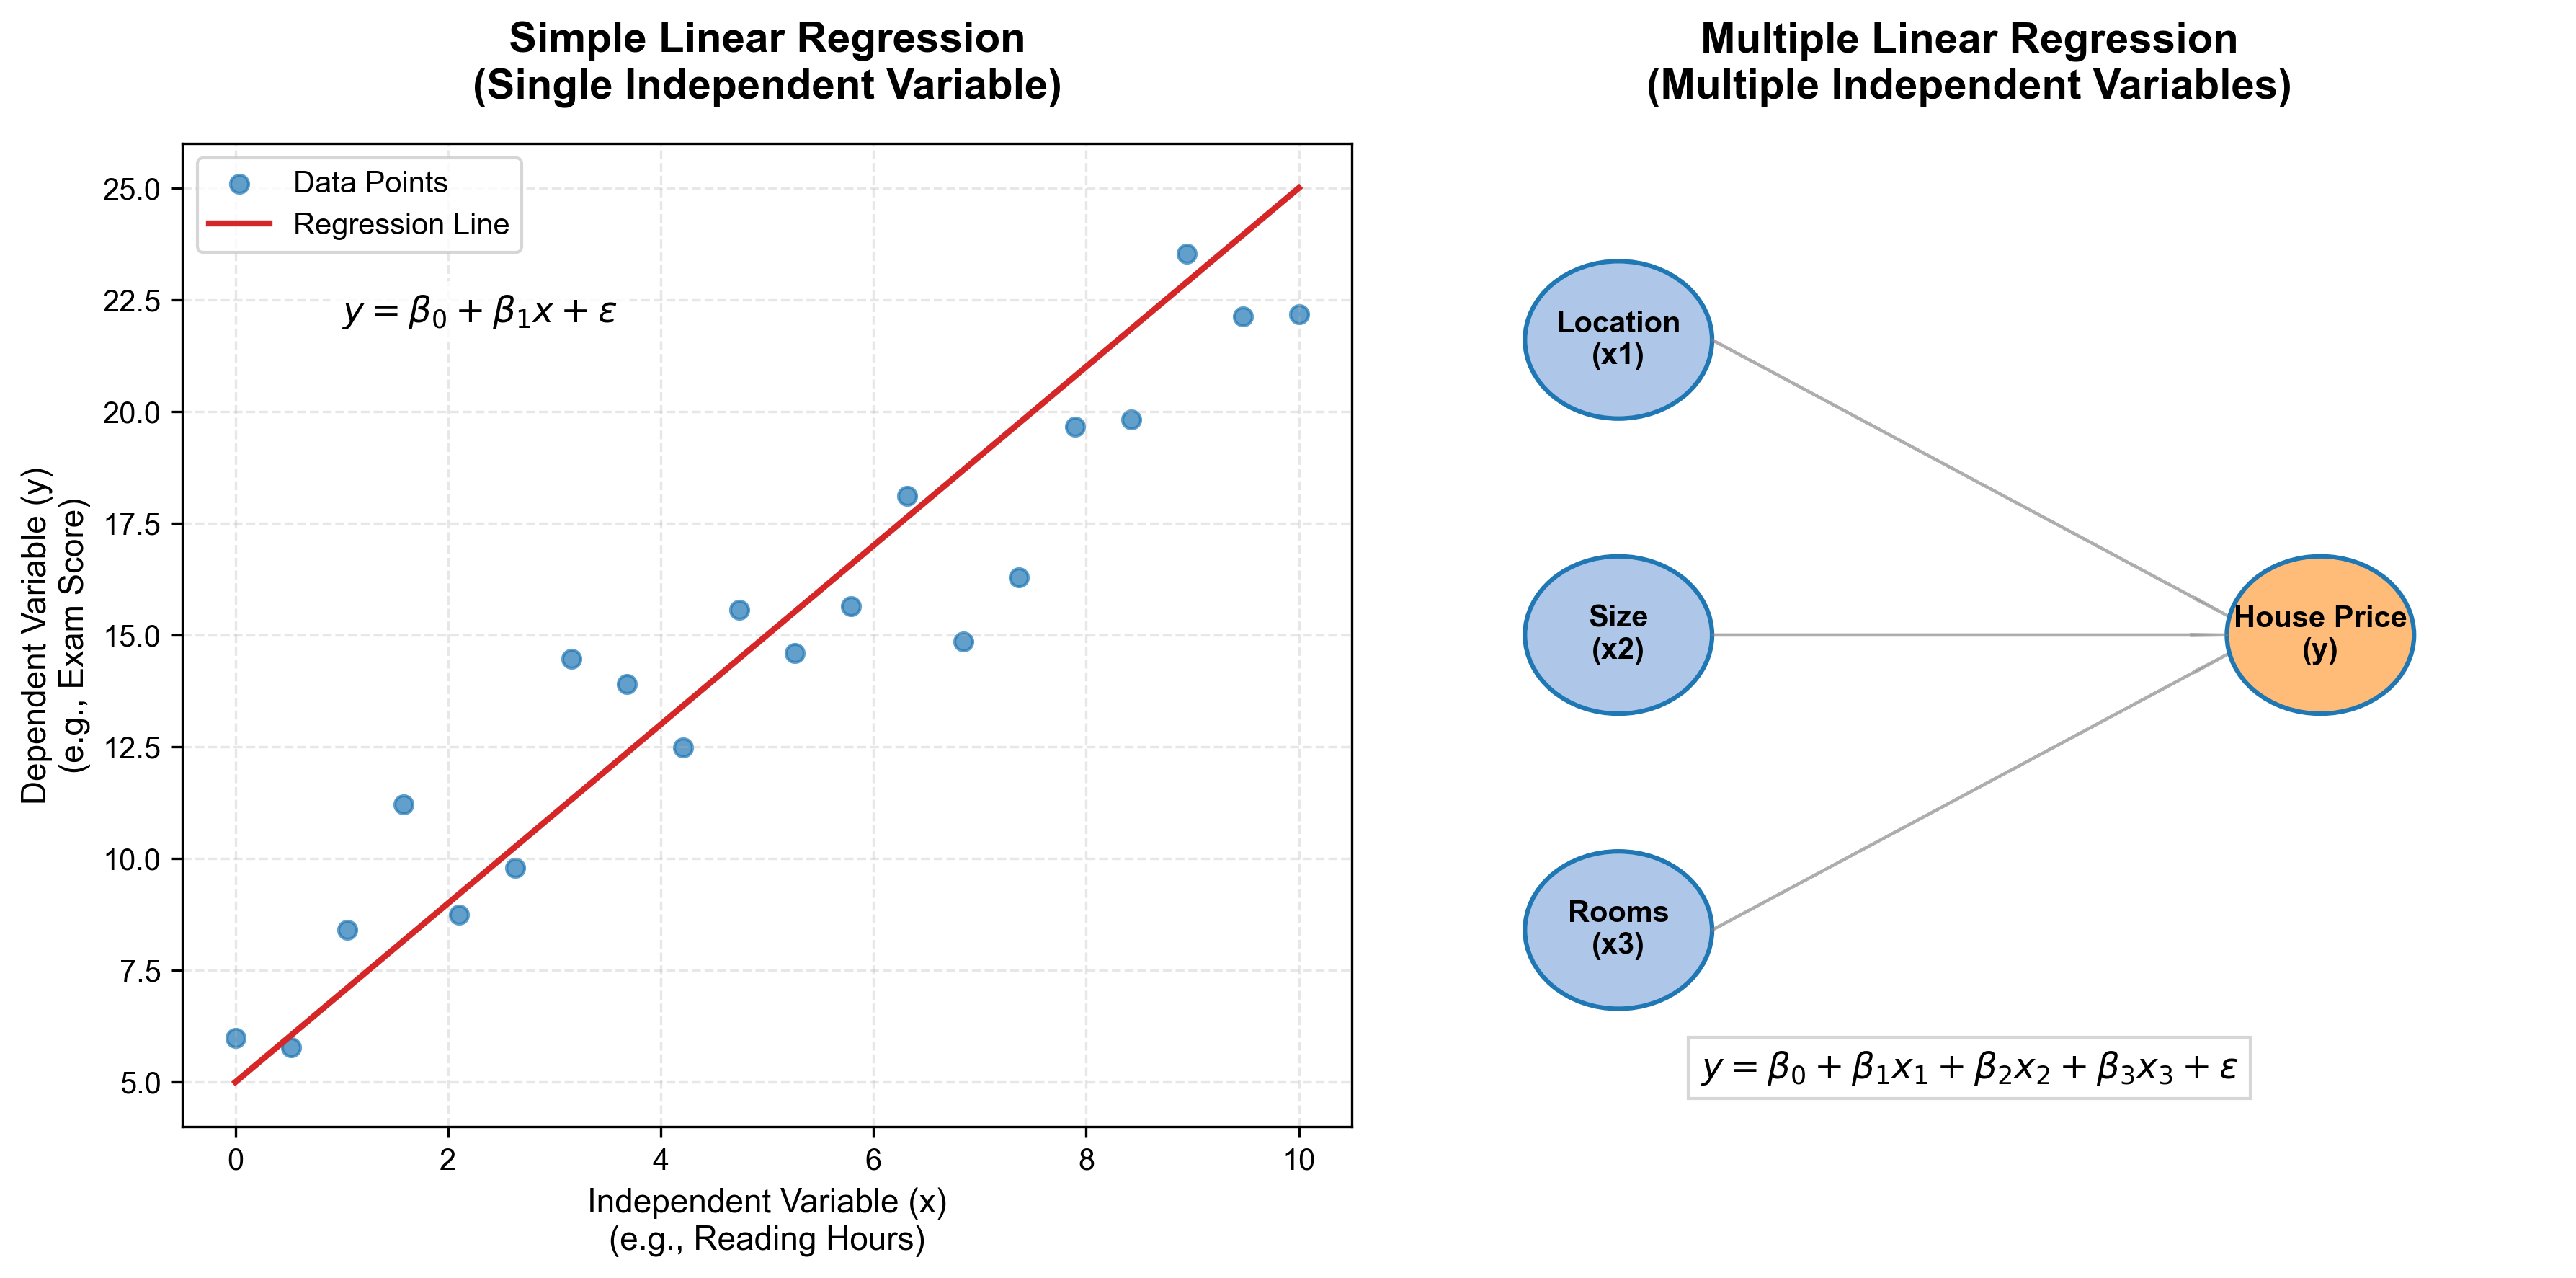
\includegraphics[width=0.95\textwidth]{regression_types_diagram.png}
\end{figure}

\noindent
\textbf{ตัวอย่างการประยุกต์ใช้การถดถอยเชิงเส้นอย่างง่าย} 

การศึกษาผลกระทบของ \textit{"จำนวนชั่วโมงในการอ่านหนังสือ"} (ตัวแปรอิสระ) ที่มีต่อ \textit{"คะแนนสอบ"} (ตัวแปรตาม) หรือการประมาณ \textit{"ระดับความสุข"} จาก \textit{"รายได้ต่อเดือน"} เพียงปัจจัยเดียว

\noindent
\textbf{ตัวอย่างการประยุกต์ใช้ะการถดถอยเชิงเส้นพหุคูณ} 

การประเมิน \textit{"ราคาขายของบ้าน"} (ตัวแปรตาม) โดยพิจารณาจากปัจจัยหลายประการร่วมกัน เช่น \textit{"ตำแหน่งที่ตั้ง"}, \textit{"จำนวนห้องนอน"}, \textit{"อายุของสิ่งปลูกสร้าง"}, และ \textit{"ขนาดพื้นที่ใช้สอย"} (ตัวแปรอิสระ) ซึ่งจะให้ผลการทำนายที่แม่นยำและสมจริงกว่าการพิจารณาเพียงปัจจัยใดปัจจัยหนึ่ง

\begin{myBox}[]{ประเภทปัญหาการถดถอย}{}
\begin{itemize}
	\item \textbf{การถดถอยเชิงเส้นอย่างง่าย (Simple Linear Regression)} 
	
	เป็นรูปแบบพื้นฐานที่สุดของการวิเคราะห์การถดถอย โดยมุ่งเน้นศึกษาความสัมพันธ์ระหว่างตัวแปรตาม กับตัวแปรอิสรเพียงตัวแปรเดียว เป้าหมายคือ การหาเส้นตรงที่สามารถเป็นตัวแทนของข้อมูลได้ดีที่สุด 
	
	\item \textbf{การถดถอยเชิงเส้นพหุคูณ (Multiple Linear Regression)} 
	
	เป็นการขยายแนวคิดจากการถดถอยอย่างง่ายเพื่อรองรับสถานการณ์จริงที่มีความซับซ้อนมากขึ้น โดยพิจารณาตัวแปรอิสระตั้งแต่ 2 สมการในกรณีนี้จะเป็นผลรวมเชิงเส้นของตัวแปรอิสระแต่ละตัว
\end{itemize}
\end{myBox}



\subsection{ความแตกต่างระหว่างการถดถอยและการจำแนกประเภท}
แม้วัตถุประสงค์หลักของการถดถอย (Regression) และการจำแนกประเภท (Classification) จะมีความคล้ายคลึงกันในการสร้างทำนายผลลัพธ์ (Prediction) จากข้อมูลนำเข้า แต่ความแตกต่างเชิงรากฐานอยู่ที่ลักษณะของ \textbf{ตัวแปรเป้าหมาย (Target Variable)}


\begin{figure}[h]
	\centering
	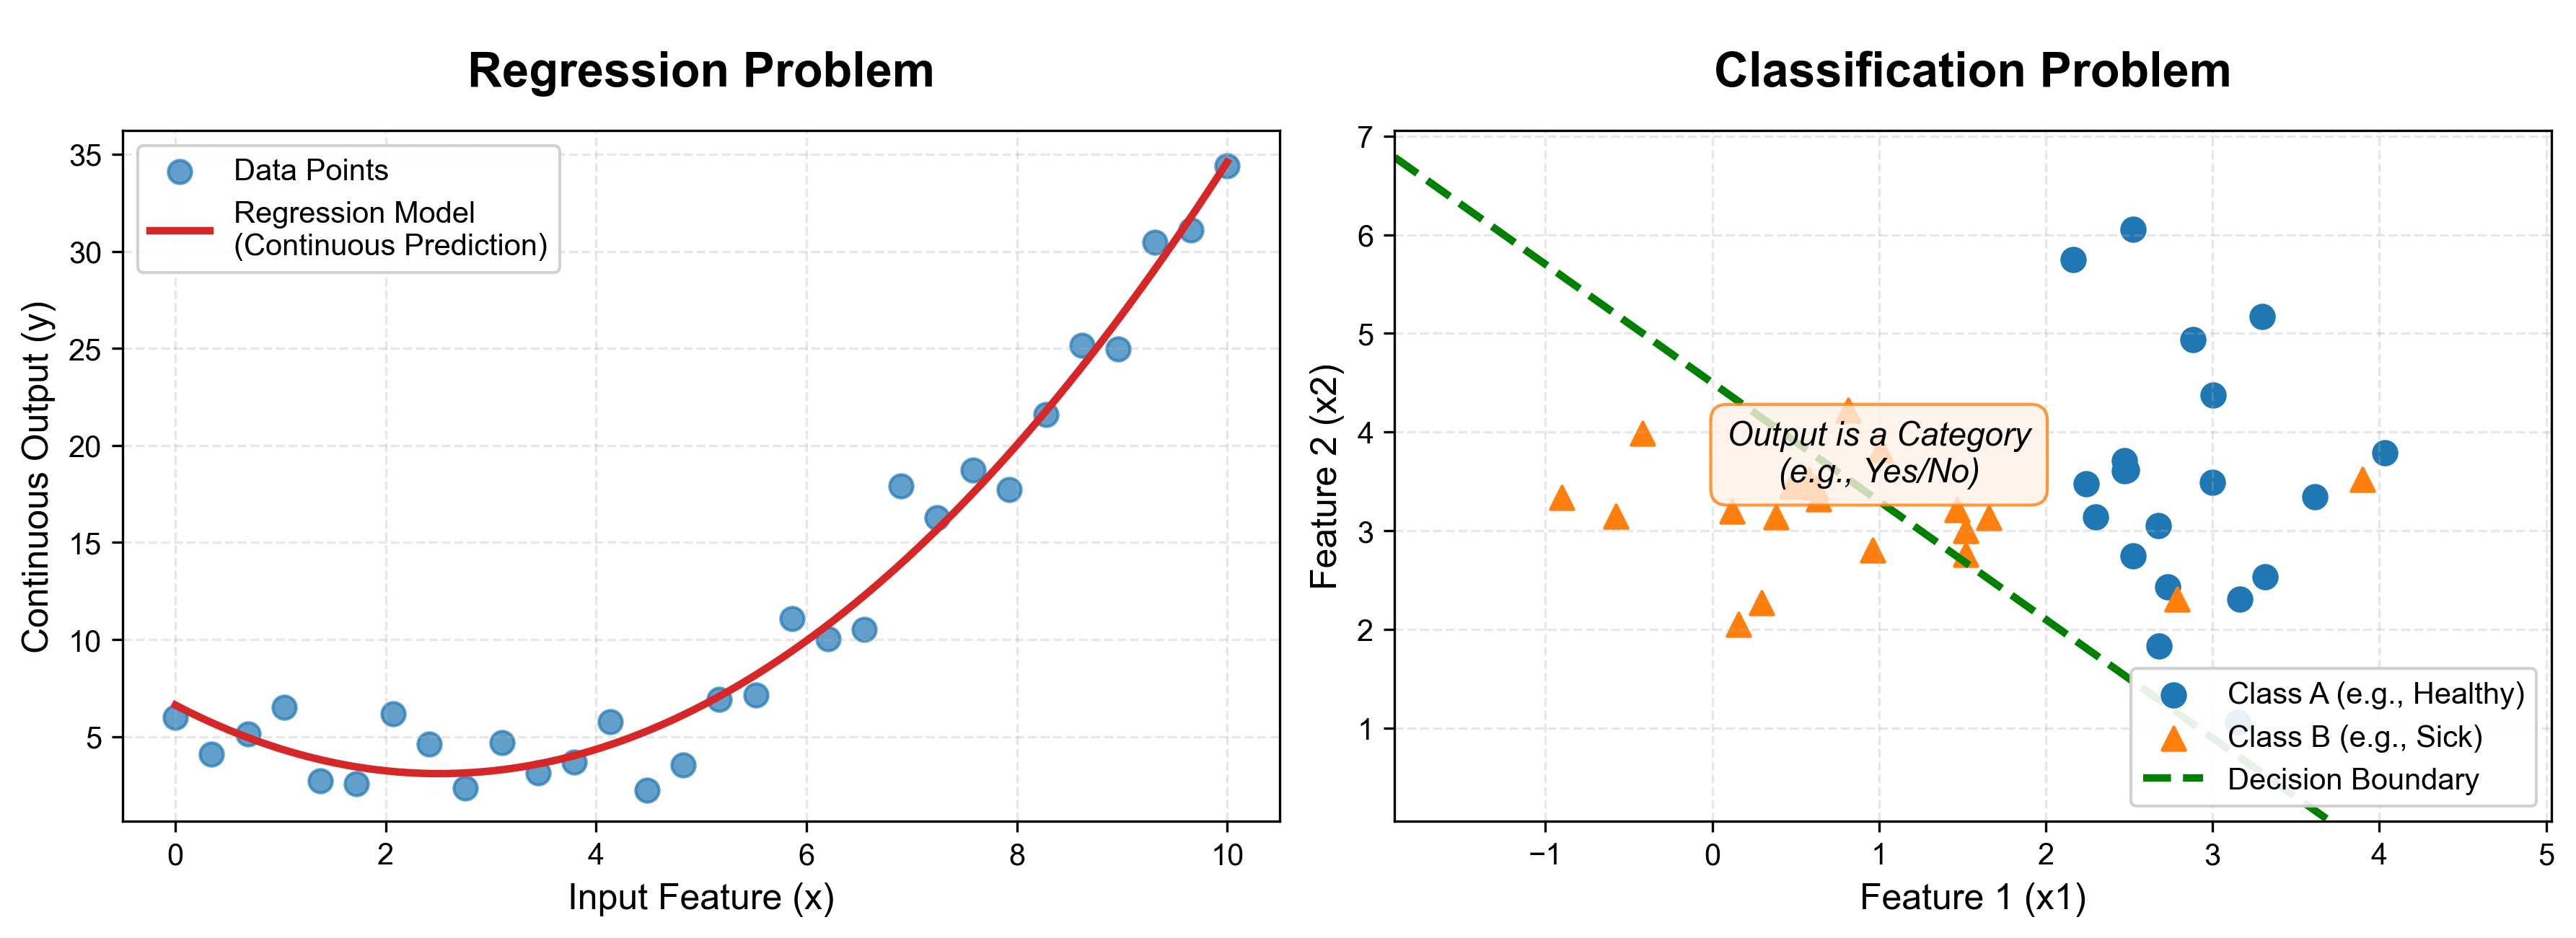
\includegraphics[width=0.95\textwidth]{reg_vs_class_diagram.png}
	\caption{การเปรียบเทียบความแตกต่างระหว่างปัญหาการถดถอย (ซ้าย) และปัญหาการจำแนกประเภท (ขวา)}
	\label{fig:reg_vs_class}
\end{figure}


\begin{myLimit}[]{ความแตกต่างระหว่างการถดถอยและการจำแนกประเภท}{}
\begin{itemize}
	\item \textbf{การถดถอย (Regression)} ใช้สำหรับทำนายข้อมูลที่มีลักษณะ \textbf{ต่อเนื่อง (Continuous)} หรือเชิงปริมาณ (Quantitative) ซึ่งผลลัพธ์สามารถเป็นค่าใด ๆ ก็ได้ในช่วงจำนวนจริง เช่น จำนวนเงิน อุณหภูมิ และ ระยะเวลา  เป็นต้น
	
	\item \textbf{การจำแนกประเภท (Classification)} ใช้สำหรับทำนายข้อมูลที่มีลักษณะ \textbf{ไม่ต่อเนื่อง (Discrete)} หรือเชิงคุณภาพ (Qualitative) ซึ่งผลลัพธ์จะเป็นการระบุกลุ่ม (Class) หรือป้ายกำกับ (Label) เช่น ใช่/ไม่ใช่, ผ่าน/ไม่ผ่าน, หรือ ประเภท A/B/C เป็นต้น
\end{itemize}
\end{myLimit}

จากข้างต้นเพื่อให้เห็นภาพความแตกต่างอย่างชัดเจน สามารถพิจารณาตัวอย่างการประยุกต์ใช้ใน 3 กรณีศึกษา ดังนี้

\begin{enumerate}
	\item[] \textbf{กรณีศึกษาทางการแพทย์}
	\begin{itemize}
		\item \textit{Regression:} การทำนาย \textit{"ระยะเวลาพักฟื้น (Recovery Days)"} โดยพิจารณาจาก \textit{"อายุของผู้ป่วย (Age)"} ซึ่งมีความสัมพันธ์ในทิศทางเดียวกัน
		\item \textit{Classification:} การวินิจฉัยสถานะ \textit{"เบาหวาน (Diabetic/Non-Diabetic)"} โดยพิจารณาจาก \textit{"ดัชนีมวลกาย (BMI)"} และ \textit{"ระดับน้ำตาลในเลือด (Glucose Level)"} ร่วมกัน
	\end{itemize}
	\begin{figure}[h]
		\centering
		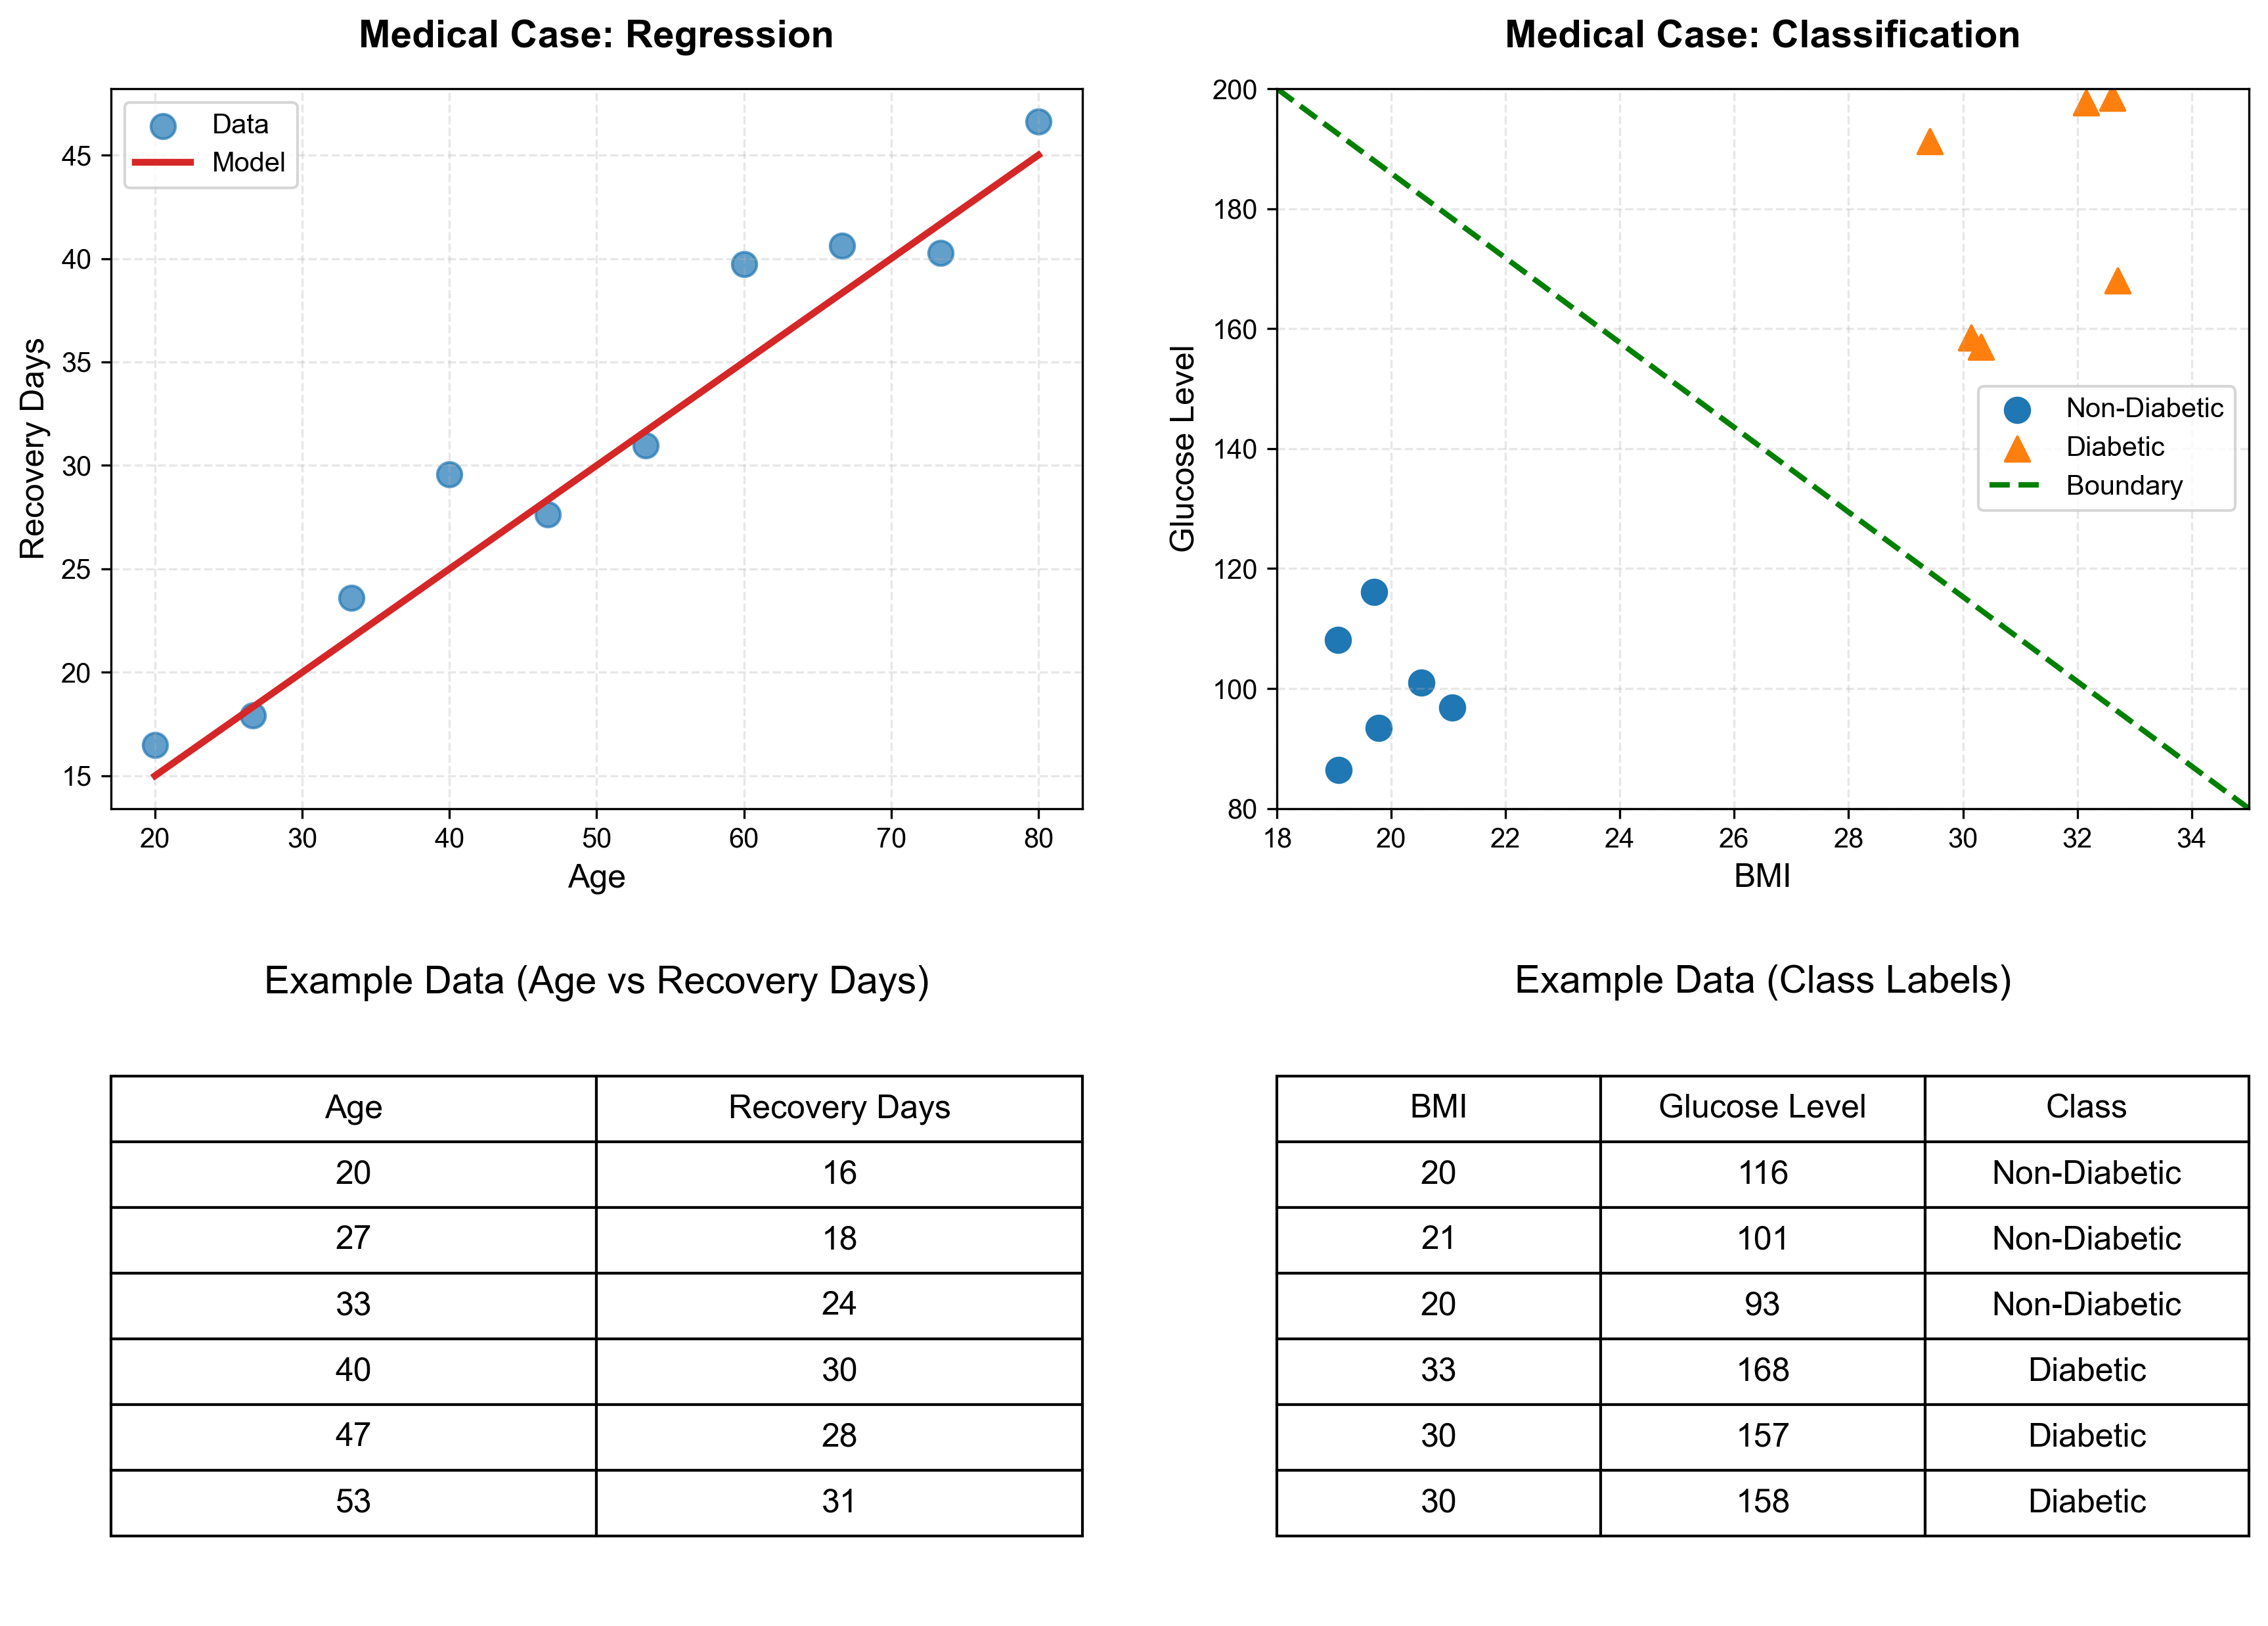
\includegraphics[width=0.8\textwidth]{case_medical.png}
		\caption{กรณีศึกษาทางการแพทย์โดยเปรียบเทียบการถดถอย (ซ้าย) และการจำแนกประเภท (ขวา)}
	\end{figure}
	
	\item[] \textbf{กรณีศึกษาด้านการตลาด}
	\begin{itemize}
		\item \textit{Regression:} การทำนาย \textit{"ยอดขายรวม (Total Sales)"} จาก \textit{"งบประมาณโฆษณา (Ad Spend)"} ซึ่งแสดงความสัมพันธ์เชิงเส้น
		\item \textit{Classification:} การทำนายการตัดสินใจซื้อ \textit{"(Will Buy/Will Not Buy)"} โดยวิเคราะห์จาก \textit{"อายุ (Age)"} และ \textit{"รายได้ต่อปี (Annual Income)"} ของลูกค้า
	\end{itemize}
	\begin{figure}[h]
		\centering
		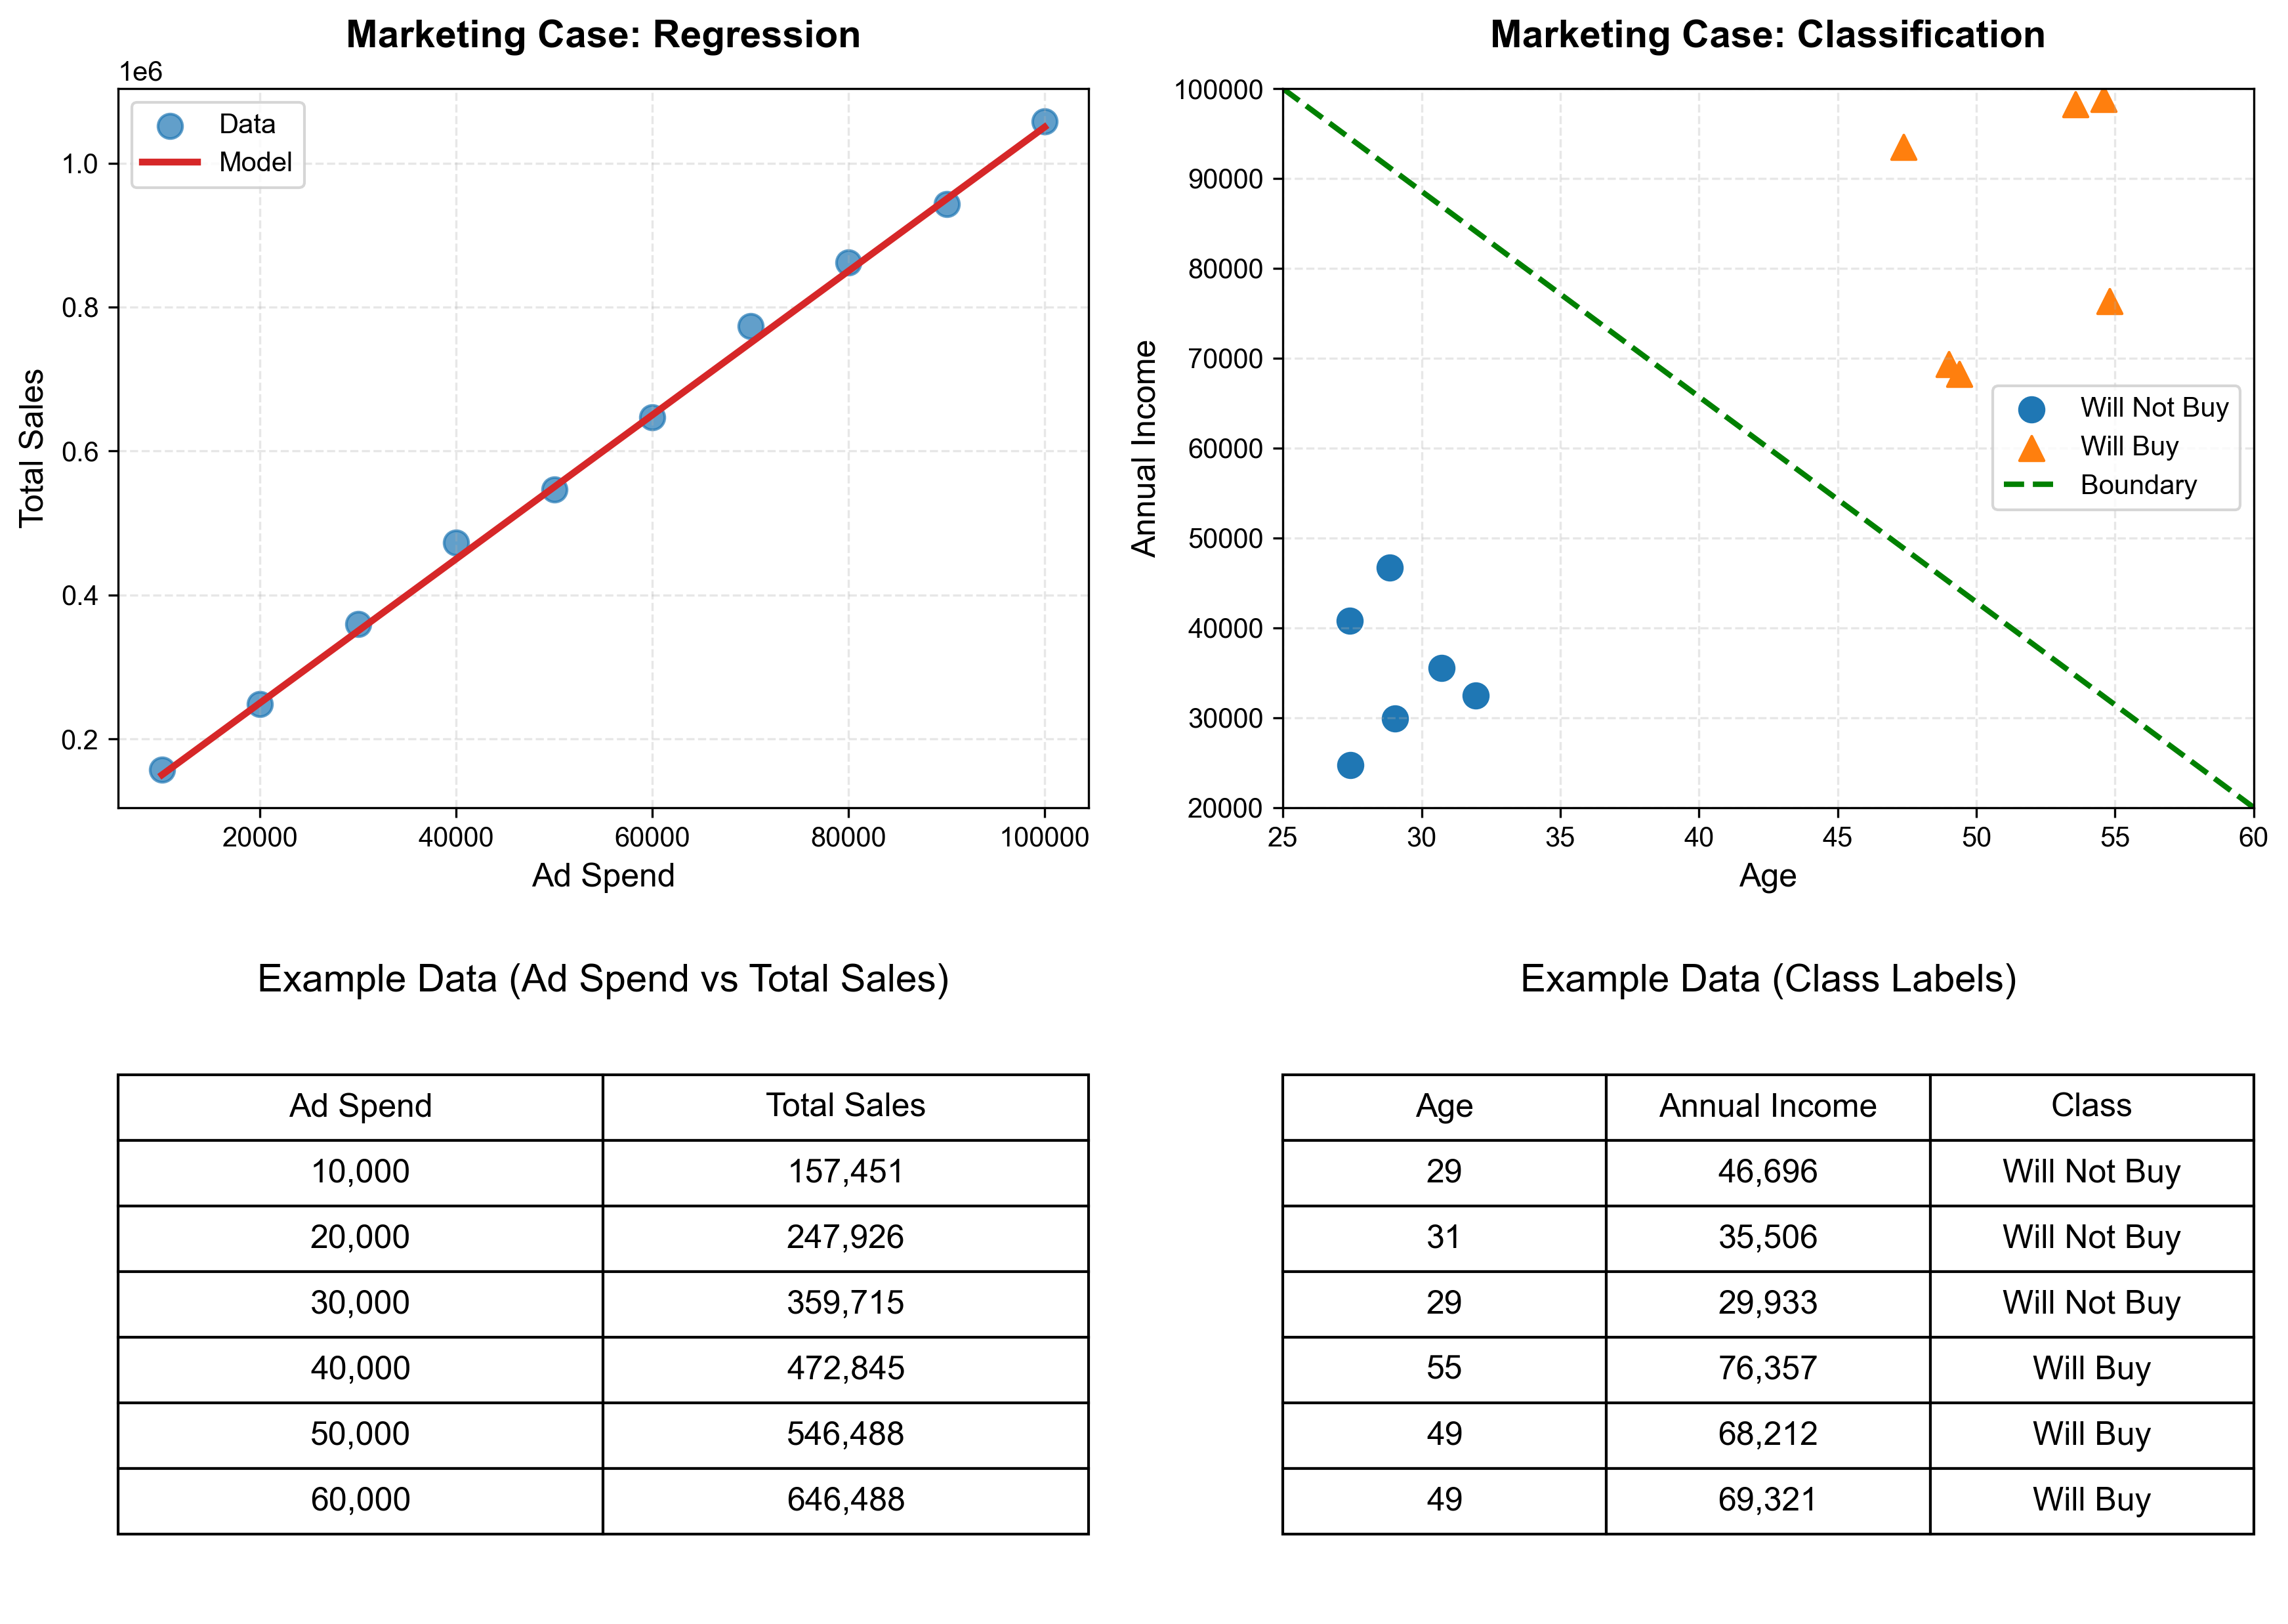
\includegraphics[width=0.8\textwidth]{case_marketing.png}
		\caption{กรณีศึกษาด้านการตลาดโดยเปรียบเทียบการถดถอย (ซ้าย) และการจำแนกประเภท (ขวา)}
	\end{figure}	

	
	\item[] \textbf{กรณีศึกษาด้านการเงิน}
	\begin{itemize}
		\item \textit{Regression:} การทำนาย \textit{"ราคาหุ้น (Stock Price)"} โดยอ้างอิงจาก \textit{"ดัชนีตลาด (Market Index)"}
		\item \textit{Classification:} การประเมินความเสี่ยง \textit{"การผิดนัดชำระหนี้ (Default/Non-Default)"} โดยพิจารณาจาก \textit{"อัตราหนี้สิน (Debt Ratio)"} และ \textit{"ระดับรายได้ (Income Level)"}
	\end{itemize}
	\begin{figure}[h]
		\centering
		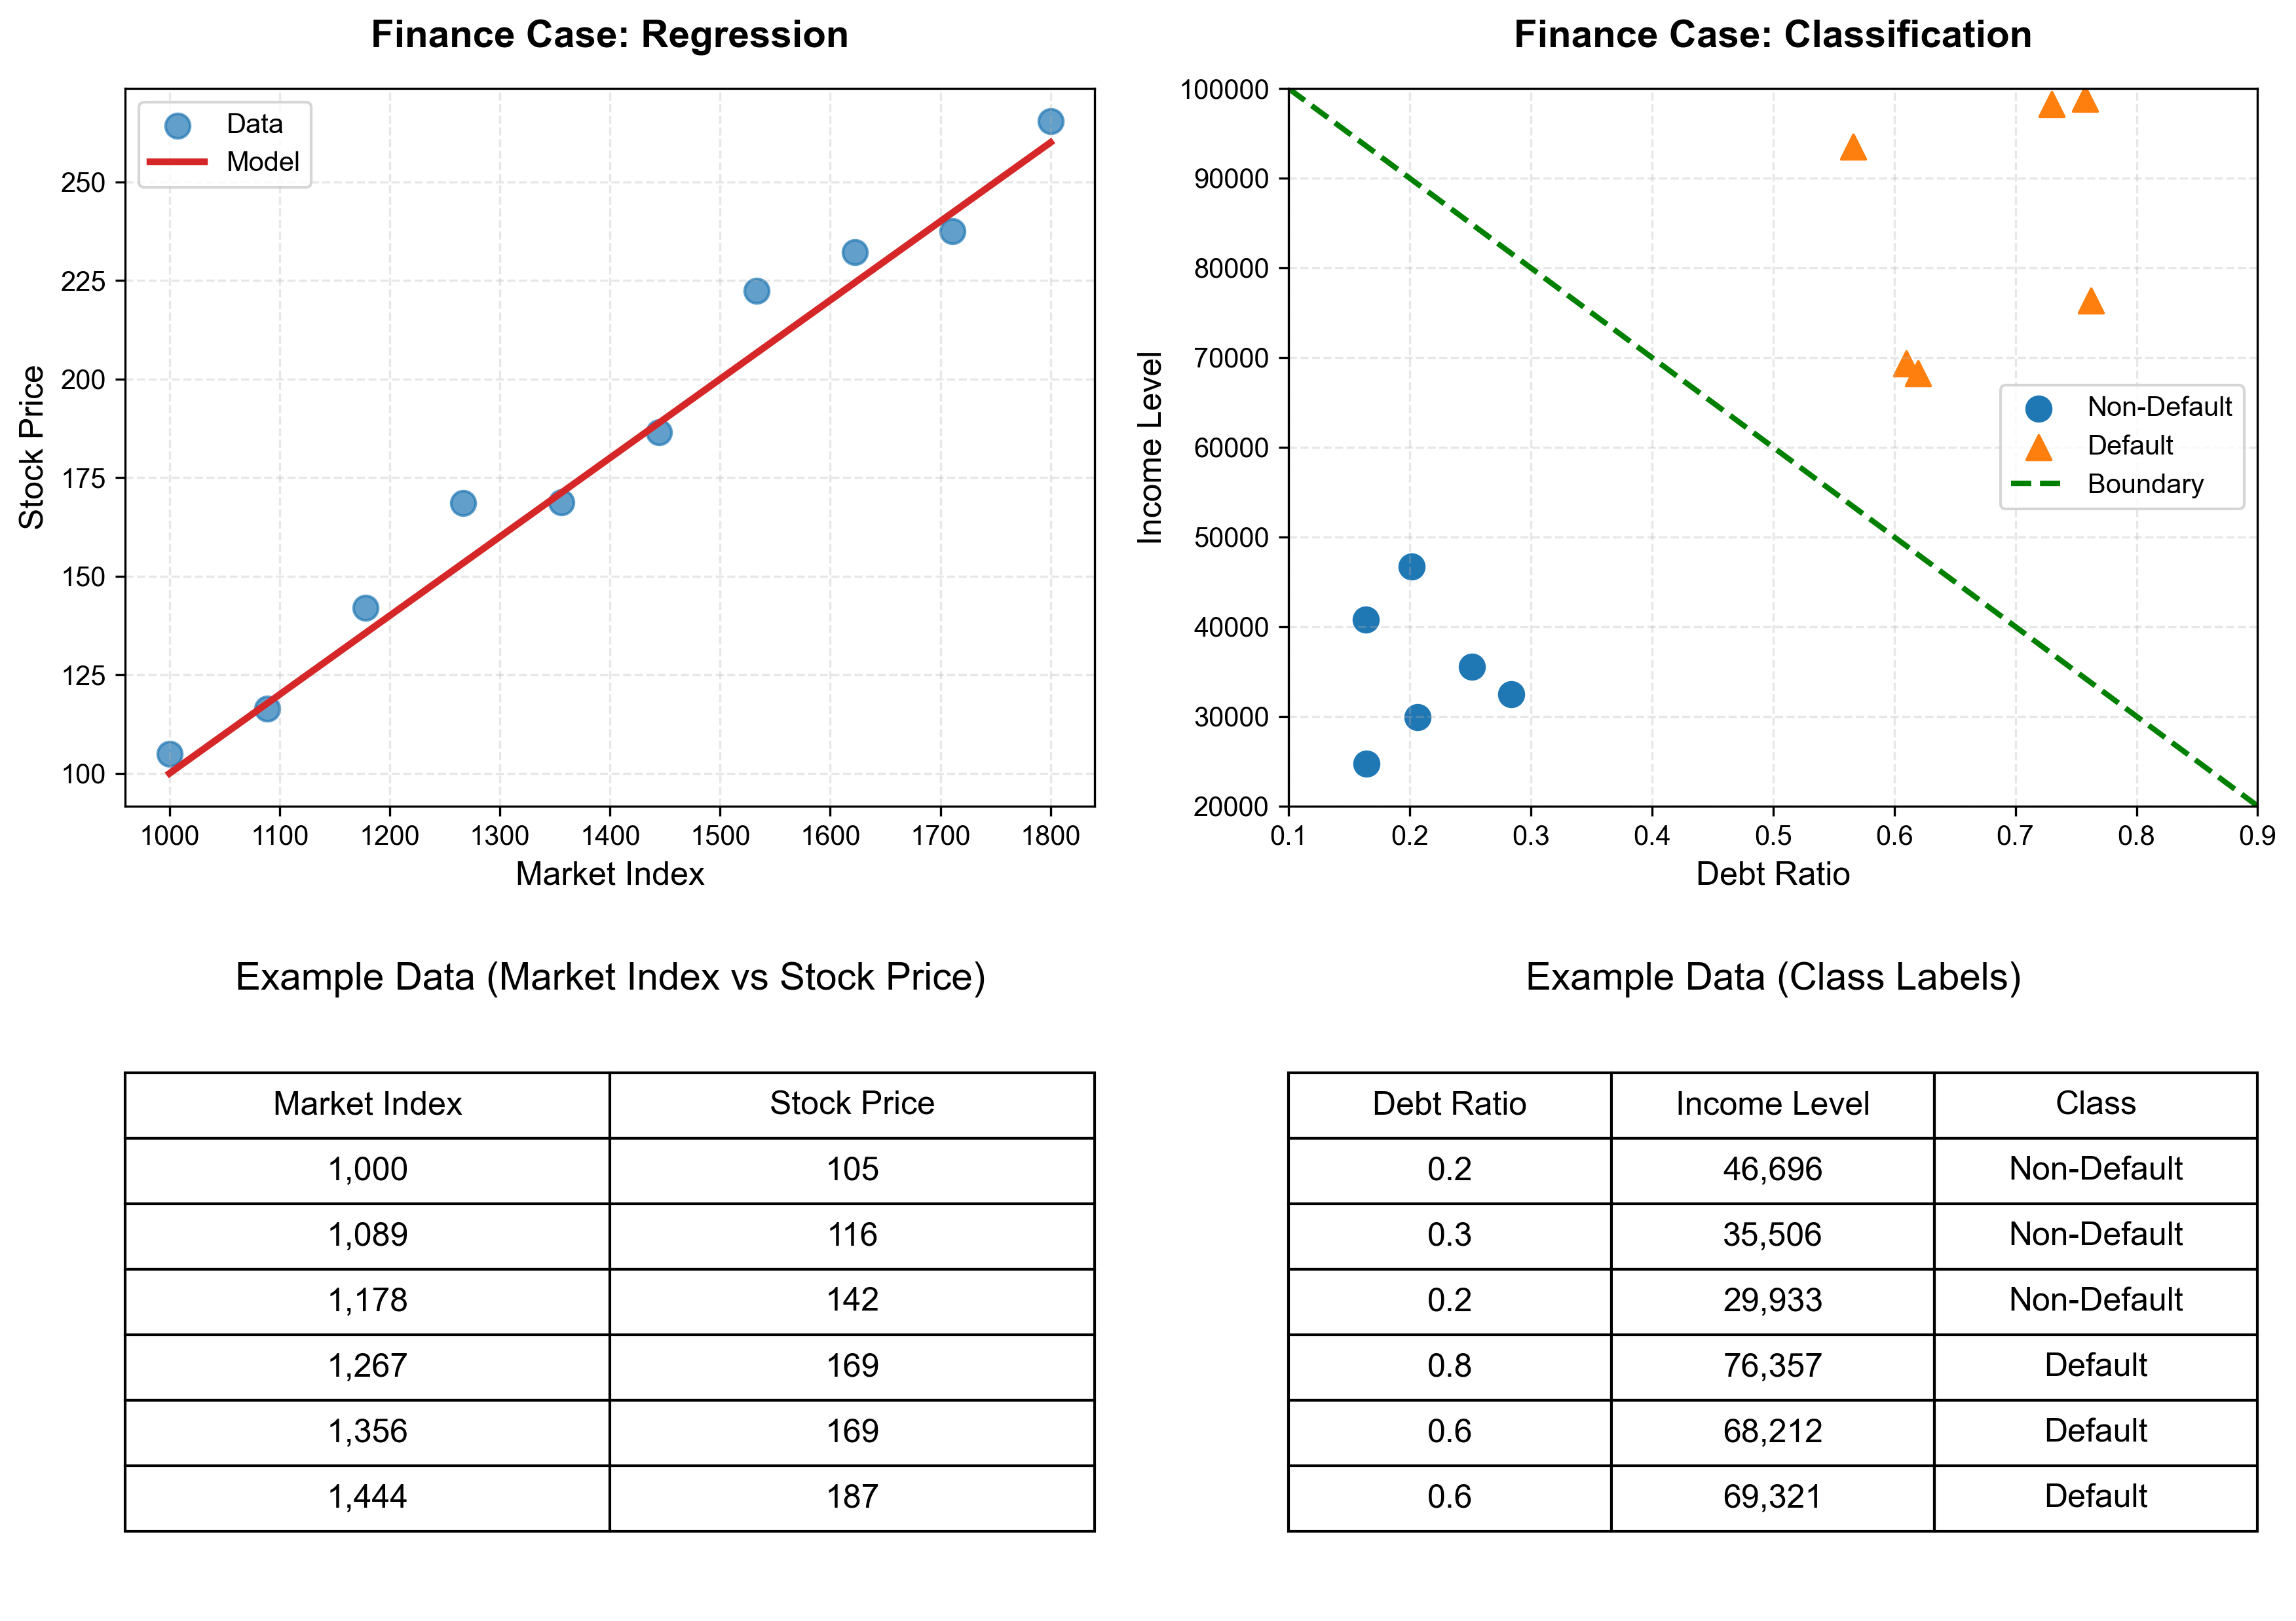
\includegraphics[width=0.8\textwidth]{case_finance.png}
		\caption{กรณีศึกษาด้านการเงินโดยเปรียบเทียบการถดถอย (ซ้าย) และการจำแนกประเภท (ขวา)}
	\end{figure}
\end{enumerate}








%####################################
\section{การถดถอยเชิงเส้นอย่างง่าย (Simple Linear Regression)}

\subsection{ตัวแบบการถดถอยเชิงเส้นอย่างง่าย}
การถดถอยเชิงเส้นอย่างง่าย (Simple Linear Regression) เป็นวิธีการทางสถิติที่ใช้สำหรับศึกษาความสัมพันธ์ระหว่างตัวแปรอิสระตัวเดียว $x$ กับตัวแปรตาม $y$ ในรูปของความสัมพันธ์เชิงเส้น ตัวแบบนี้เป็นพื้นฐานที่สำคัญสำหรับการทำความเข้าใจการวิเคราะห์การถดถอยในเชิงลึกต่อไป

ตัวแบบการถดถอยเชิงเส้นอย่างง่ายมีรูปแบบดังนี้

\[
y = \beta_0 + \beta_1 x + \varepsilon
\]

โดยที่ $\beta_0$ คือจุดตัดแกน (Intercept) ซึ่งเป็นค่าของ $y$ เมื่อ $x = 0$ และ $\beta_1$ คือความชัน (Slope) ซึ่งแสดงการเปลี่ยนแปลงของ $y$ เมื่อ $x$ เพิ่มขึ้น 1 หน่วย $\varepsilon$ คือค่าความคลาดเคลื่อน (Error Term) ที่เป็นตัวแทนของความผิดพลาดในการทำนายที่ไม่สามารถอธิบายได้ด้วยความสัมพันธ์เชิงเส้น

\begin{exmp}
\label{exmp:simple_linear_regression_study_hours}
พิจารณาตัวอย่างการศึกษาความสัมพันธ์ระหว่างจำนวนชั่วโมงการอ่านหนังสือต่อวันกับคะแนนสอบของนักศึกษา 8 คน ดังตาราง \ref{tab:study_hours_data}

\begin{table}[h!]
\centering
\caption{ข้อมูลจำนวนชั่วโมงอ่านหนังสือและคะแนนสอบของนักศึกษา 8 คน}
\label{tab:study_hours_data}
\begin{tabular}{|c|c|c|}
\hline
\textbf{นักศึกษา} & \textbf{ชั่วโมงอ่านต่อวัน ($x$)} & \textbf{คะแนนสอบ ($y$)} \\ \hline
1 & 1.0 & 45 \\ \hline
2 & 2.0 & 52 \\ \hline
3 & 3.0 & 58 \\ \hline
4 & 3.5 & 65 \\ \hline
5 & 4.0 & 70 \\ \hline
6 & 4.5 & 75 \\ \hline
7 & 5.5 & 82 \\ \hline
8 & 6.0 & 88 \\ \hline
\end{tabular}
\end{table}

จากข้อมูลในตาราง สมมติได้สมการถดถอย $\hat{y} = 33.2 + 9.1x$ หมายความว่าทุก 1 ชั่วโมงที่เพิ่มขึ้น คะแนนสอบจะเพิ่มขึ้นประมาณ 9.1 คะแนน และเมื่อ $x = 0$ ค่าคะแนนพยากรณ์เบื้องต้นคือ 33.2 คะแนน
\end{exmp}

\subsection{วิธีกำลังสองน้อยที่สุด (Least Squares Method)}
วิธีกำลังสองน้อยที่สุด (Ordinary Least Squares: OLS) เป็นวิธีมาตรฐานในการประมาณค่าพารามิเตอร์ $\beta_0$ และ $\beta_1$ ของตัวแบบการถดถอยเชิงเส้น โดยมีหลักการคือการเลือกค่า $\hat{\beta}_0$ และ $\hat{\beta}_1$ ที่ทำให้ผลรวมของค่าความคลาดเคลื่อนยกกำลังสอง (Residual Sum of Squares: RSS) มีค่าน้อยที่สุด

\[
\text{RSS} = \sum_{i=1}^{n}(y_i - \hat{y}_i)^2 = \sum_{i=1}^{n}\left(y_i - \hat{\beta}_0 - \hat{\beta}_1 x_i\right)^2
\]

\begin{exmp}
\label{exmp:ols_calculation}
จากข้อมูลในตัวอย่าง \ref{exmp:simple_linear_regression_study_hours} การคำนวณค่า $\hat{\beta}_0$ และ $\hat{\beta}_1$ ด้วยวิธี OLS มีขั้นตอนดังนี้

จากสูตร

\[
\hat{\beta}_1 = \frac{\sum_{i=1}^{n}(x_i - \bar{x})(y_i - \bar{y})}{\sum_{i=1}^{n}(x_i - \bar{x})^2}, \qquad
\hat{\beta}_0 = \bar{y} - \hat{\beta}_1 \bar{x}
\]

โดยมีค่าเฉลี่ย $\bar{x} = 3.69$ และ $\bar{y} = 66.88$ จากการคำนวณจะได้

\[
\hat{\beta}_1 = \frac{269.5}{29.63} \approx 9.09, \qquad \hat{\beta}_0 = 66.88 - 9.09(3.69) \approx 33.3
\]

ดังนั้นสมการถดถอยคือ $\hat{y} = 33.3 + 9.09x$
\end{exmp}

\subsection{การตีความค่าสัมประสิทธิ์}
การตีความค่าสัมประสิทธิ์การถดถอยเป็นส่วนสำคัญในการวิเคราะห์ผลลัพธ์ ค่า $\hat{\beta}_1$ แสดงการเปลี่ยนแปลงโดยเฉลี่ยของตัวแปรตาม $y$ เมื่อตัวแปรอิสระ $x$ เพิ่มขึ้น 1 หน่วย โดยที่ตัวแปรอื่น ๆ คงที่ (Ceteris Paribus)

\begin{exmp}
\label{exmp:coefficient_interpretation}
จากสมการถดถอยในตัวอย่าง \ref{exmp:simple_linear_regression_study_hours} ค่า $\hat{\beta}_1 = 9.09$ หมายความว่าเมื่อนักศึกษาอ่านหนังสือเพิ่มขึ้น 1 ชั่วโมงต่อวัน คะแนนสอบจะเพิ่มขึ้นโดยเฉลี่ย 9.09 คะแนน ค่า $\hat{\beta}_0 = 33.3$ หมายความว่าหากนักศึกษาไม่อ่านหนังสือเลย ($x = 0$) คะแนนสอบที่พยากรณ์ได้คือ 33.3 คะแนน อย่างไรก็ตาม ค่านี้อาจไม่มีความหมายในทางปฏิบัติเนื่องจากการ extrapolate ไปนอกช่วงของข้อมูลที่สังเกต
\end{exmp}

\subsection{การประเมินประสิทธิภาพของโมเดล}
การประเมินประสิทธิภาพของตัวแบบการถดถอยเชิงเส้นใช้ตัวชี้วัดหลายตัว ได้แก่ $R^2$ (Coefficient of Determination) ซึ่งแสดงสัดส่วนของความแปรปรวนของ $y$ ที่สามารถอธิบายได้ด้วยตัวแบบ และ RMSE (Root Mean Squared Error) ซึ่งแสดงค่าเบี่ยงเบนเฉลี่ยของค่าทำนายจากค่าจริงในหน่วยเดียวกับ $y$

\begin{exmp}
\label{exmp:r_squared_calculation}
จากข้อมูลในตัวอย่าง \ref{exmp:simple_linear_regression_study_hours} สมมติได้ค่า $\hat{y}$ จากสมการ $\hat{y} = 33.3 + 9.09x$ ดังนี้

\begin{table}[h!]
\centering
\caption{ค่าทำนายและค่าคงเหลือจากสมการถดถอย}
\label{tab:residual_calc}
\begin{tabular}{|c|c|c|c|c|}
\hline
$x$ & $y$ & $\hat{y}$ & $y - \hat{y}$ & $(y - \hat{y})^2$ \\ \hline
1.0 & 45 & 42.4 & 2.6 & 6.76 \\ \hline
2.0 & 52 & 51.5 & 0.5 & 0.25 \\ \hline
3.0 & 58 & 60.6 & $-2.6$ & 6.76 \\ \hline
3.5 & 65 & 65.1 & $-0.1$ & 0.01 \\ \hline
4.0 & 70 & 69.7 & 0.3 & 0.09 \\ \hline
4.5 & 75 & 74.2 & 0.8 & 0.64 \\ \hline
5.5 & 82 & 83.3 & $-1.3$ & 1.69 \\ \hline
6.0 & 88 & 87.8 & 0.2 & 0.04 \\ \hline
\end{tabular}
\end{table}

จากตาราง ค่า RMSE คำนวณได้จาก

\[
\text{RMSE} = \sqrt{\frac{\sum(y_i - \hat{y}_i)^2}{n}} = \sqrt{\frac{16.24}{8}} \approx 1.43 \text{ คะแนน}
\]

และสามารถคำนวณค่า $R^2 \approx 0.975$ ซึ่งหมายความว่าตัวแบบสามารถอธิบายความแปรปรวนของคะแนนสอบได้ประมาณ 97.5\%
\end{exmp}




%####################################
\section{การถดถอยเชิงเส้นพหุคูณ (Multiple Linear Regression)}
การถดถอยเชิงเส้นพหุคูณ (Multiple Linear Regression) เป็นการขยายแนวคิดจากการถดถอยเชิงเส้นอย่างง่ายเพื่อรองรับสถานการณ์จริงที่มีความซับซ้อน ซึ่งปรากฏการณ์ที่สนใจมักถูกกำหนดโดยตัวแปรอิสระ (Independent Variables) มากกว่าหนึ่งตัวพร้อมกัน ทำให้ตัวแบบสามารถจับความสัมพันธ์ระหว่างตัวแปรตาม $Y$ กับตัวแปรอิสระ $k$ ตัว ได้แก่ $x_1, x_2, \ldots, x_k$ ในรูปของผลรวมเชิงเส้น (Linear Combination) ของสัมประสิทธิ์การถดถอย (Regression Coefficients) $\boldsymbol{\beta}$ ซึ่งต้องได้รับการประมาณค่าจากข้อมูลตัวอย่าง เนื้อหาในหัวข้อนี้จะนำเสนอ \textbf{ตัวแบบการถดถอยเชิงเส้นพหุคูณ} ในรูปสมการและสัญกรณ์เมทริกซ์ที่กะทัดรัดและเป็นสากล รวมถึงวิเคราะห์ \textbf{ข้อจำกัดสำคัญของตัวแบบ} ที่เกิดจากสมมติฐานความเป็นเชิงเส้น อันนำไปสู่ปัญหาการทำนายค่านอกช่วงที่เป็นไปได้ (Out-of-Range Prediction) และการละเมิดสมมติฐานความแปรปรวนสม่ำเสมอ (Homoscedasticity) โดยเฉพาะอย่างยิ่งเมื่อตัวแปรตามมีลักษณะเชิงคุณภาพแบบทวิภาค ซึ่งข้อจำกัดเหล่านี้เป็นพื้นฐานสำคัญที่ชี้ให้เห็นถึงความจำเป็นในการพัฒนาตัวแบบขั้นสูงอย่างการถดถอยโลจิสติค (Logistic Regression) ในหัวข้อถัดไป


\newpage
\begin{myBox}[]{ตัวแบบถดถอยเชิงเส้นเส้นพหุ}{}
กำหนดให้ $D=\{(\bx_i, \by_i)\}_{i=1}^n $ แทนข้อมูลการฝึกสอนขนาด $n$ สำหรับตัวแบบการถดถอยเชิงเส้นพหุ (Multiple linear regression model) มีรูปแบบทั่วไป คือ

\begin{equation}
	Y_i = \beta_0 + \beta_1 x_{1i} + \beta_2 x_{2i} + \cdots + \beta_k x_{ki} + \varepsilon_i
\end{equation}

ซึ่งสามารถเขียนในรูปของเมทริกซ์ ดังนี้

\begin{eqnarray} \nonumber
	\bm{Y} &=& \mathbf{X}^{T}\bbeta + \bm{\epsilon} \\
	\begin{bmatrix}
		y_{1} \\
		y_{2} \\
		\vdots \\
		y_{n} \\
	\end{bmatrix}_{n\times1}  &=& 	
	\begin{bmatrix}
		1 & x_{11} & x_{21} & \cdots & x_{k1} \\
		1 & x_{12} & x_{22} & \cdots & x_{k2} \\
		\vdots & \vdots & \vdots & \ddots & \vdots \\
		1 & x_{1n} & x_{2n} & \cdots & x_{kn}
	\end{bmatrix}_{n\times (k+1)}\begin{bmatrix}
	\beta_{0}\\
	\beta_{1} \\
	\beta_{2} \\
	\vdots \\
	\beta_{k} \\
	\end{bmatrix}_{(k+1)\times1} + \begin{bmatrix}
	\epsilon_{1} \\
	\epsilon_{2} \\
	\vdots \\
	\epsilon_{n} \\
	\end{bmatrix}_{n\times1}
\end{eqnarray}


โดยที่

\indent\indent
$ํ\bm{Y}=\by_i=(y_{1}, y_{2}, \ldots, y_{n})^T=\begin{bmatrix}
	y_{1} \\
	y_{2} \\
	\vdots \\
	y_{n} \\
\end{bmatrix}$ แทนเวกเตอร์ของตัวแปรตาม (Dependence variable)
\end{myBox}
\begin{myBox}[]{ตัวแบบถดถอยเชิงเส้นเส้นพหุ}{}

\indent\indent
$\bx_i = (1, x_{0i},x_{1i}, x_{2i}, \ldots, x_{ki})^T$ แทนตัวแปรอิสระ (Independence variable or input feature) คุณลักษณะที่ $k$ สำหรับชุดข้อมูลที่ $i$
โดยที่ $x_{0i}=1$ หรือสามารถเขียนในรูปเมทริกซ์ ดังนี้

$$\bX=\bx_i=\begin{bmatrix}
	1 & 1 & \cdots  & 1 \\
	x_{11}& x_{12}& \cdots  & x_{1n} \\
	x_{21}& x_{22}& \cdots & x_{2n}  \\
	\vdots & \vdots  & \ddots  & \vdots  \\
	x_{k1}& x_{k2} & \cdots  & x_{kn} \\
\end{bmatrix}$$

\indent\indent
$\bbeta = (\beta_0, \beta_1, \beta_2, \ldots, \beta_k)^T=\begin{bmatrix}
	\beta_{0}\\
	\beta_{1} \\
	\beta_{2} \\
	\vdots \\
	\beta_{k} \\
\end{bmatrix}$ แทนเวกเตอร์ของสัมประสิทธิ์การถดถอย (พารามิเตอร์) ที่ไม่ทราบค่า หรือค่าถ่วงน้ำหนัก (Weight) ในทางเทคนิคการเรียนรู้ของเครื่อง

\indent\indent
$\bm{\epsilon}=(\epsilon_1, \epsilon_2, \ldots, \epsilon_n)^T=\begin{bmatrix}
	\epsilon_{1} \\
	\epsilon_{2} \\
	\vdots \\
	\epsilon_{n} \\
\end{bmatrix}$ เป็นความคลาดเคลื่อนเชิงสุ่ม (Random error)
\end{myBox}


ตัวแบบนี้อาศัยสมมติฐานหลายประการ อาทิเช่น ความเป็นเชิงเส้นของความสัมพันธ์ การกระจายแบบปกติของข้อผิดพลาด และความคงที่ของความแปรปรวน (Homoscedasticity) นอกจากนี้เมื่อตัวแปรตามเป็นตัวแปรเชิงคุณภาพแบบทวิภาค (Binary) ที่มีค่าเป็น 0 หรือ 1 เท่านั้น


\begin{myLimit}[]{ข้อจำกัดการถดถอยเชิงเส้นพหุ}{} การประยุกต์ใช้ตัวแบบการถดถอยเชิงเส้นมีข้อจำกัดหลายประการ ดังนี้
	
	\begin{itemize}
		\item ปัญหาแรกและสำคัญที่สุดคือปัญหาการทำนายค่านอกช่วงที่เป็นไปได้ (Out-of-Range Prediction) เนื่องจากค่าทำนาย $\widehat{\by}_i = \mathbf{X}^{T} \widehat{\boldsymbol{\beta}}$ มีค่าในช่วง $(-\infty, \infty)$ ในขณะที่ตัวแปรตามที่เป็นความน่าจะเป็นควรจะมีค่าอยู่ในช่วง $[0, 1]$ เท่านั้น การได้ค่าทำนายเป็น -0.3 หรือ 1.7 จึงไม่สามารถตีความเป็นความน่าจะเป็นได้อย่างสมเหตุสมผล
		
		\item ปัญหาสองคือ ส่วนเหลือ  $\varepsilon_i = Y_i - \widehat{\by}_i = Y_i -  \mathbf{X}^{T} \widehat{\boldsymbol{\beta}}$ ในกรณีของตัวแปรตามแบบทวิภาคจะไม่มีการแจกแจงปกติ เนื่องจาก $Y_i$ สามารถมีค่าเป็น 0 หรือ 1 เท่านั้น ความแปรปรวนของข้อผิดพลาดจึงขึ้นอยู่กับค่าของ $\mathbf{X}^{T} \boldsymbol{\beta}$ ทำให้เกิดปัญหา Heteroscedasticity อย่างหลีกเลี่ยงไม่ได้ จึงทำให้ไม่เป็นไปตามสมมติฐานของการถดถอยเชิงเส้น ส่งผลให้การประมาณค่าพารามิเตอร์และการทดสอบสมมติฐานสถิติไม่มีความเที่ยงตรงและไม่มีประสิทธิภาพ
	\end{itemize}
	โดยที่ $\widehat{\by}_i=(\hat{y}_{1}, \hat{y}_{2}, \ldots, \hat{y}_{n})^T$ แทนค่าการทำนายของตัวแปรตาม และ $\widehat{\bbeta}=(\hat{\beta}_{1}, \hat{\beta}_{2}, \ldots, \hat{\beta}_{k})^T$
	แทนค่าประมาณของพารามิเตอร์ $\bbeta$
\end{myLimit}

\begin{exmp}
\label{exmp:multiple_linear_regression_housing}
พิจารณาตัวอย่างการพยากรณ์ราคาบ้าน ($y$ หน่วย: ล้านบาท) โดยใช้ตัวแปรอิสระ 2 ตัว ได้แก่ ขนาดพื้นที่ใช้สอย ($x_1$ ตารางเมตร) และจำนวนห้องนอน ($x_2$) ของบ้าน 5 หลัง ดังตาราง \ref{tab:housing_data}

\begin{table}[h!]
\centering
\caption{ข้อมูลราคาบ้าน ขนาดพื้นที่ และจำนวนห้องนอน}
\label{tab:housing_data}
\begin{tabular}{|c|c|c|c|}
\hline
\textbf{บ้าน} & $x_1$ (ตร.ม.) & $x_2$ (ห้องนอน) & $y$ (ล้านบาท) \\ \hline
1 & 80 & 2 & 3.2 \\ \hline
2 & 100 & 3 & 4.5 \\ \hline
3 & 120 & 3 & 5.0 \\ \hline
4 & 150 & 4 & 6.8 \\ \hline
5 & 200 & 5 & 8.5 \\ \hline
\end{tabular}
\end{table}

สมมติได้สมการถดถอยเชิงเส้นพหุคูณ $\hat{y} = 0.5 + 0.03x_1 + 0.4x_2$ การตีความคือ เมื่อขนาดพื้นที่เพิ่มขึ้น 1 ตารางเมตร โดยที่จำนวนห้องนอนคงที่ ราคาบ้านจะเพิ่มขึ้น 0.03 ล้านบาท และเมื่อจำนวนห้องนอนเพิ่มขึ้น 1 ห้อง โดยที่ขนาดพื้นที่คงที่ ราคาบ้านจะเพิ่มขึ้น 0.4 ล้านบาท
\end{exmp}


\section{การถดถอยโลจิสติก}
การถดถอยโลจิสติก (Logistic Regression) เป็นตัวแบบทางสถิติที่ได้รับการพัฒนาขึ้นเพื่อแก้ไขข้อจำกัดเชิงโครงสร้างของการถดถอยเชิงเส้นในกรณีที่ตัวแปรตามมีลักษณะเชิงคุณภาพแบบทวิภาค (Binary Qualitative Response) โดยอาศัยกรอบแนวคิดของ Generalized Linear Model (GLM) ที่นำ\textbf{ฟังก์ชันเชื่อมโยง (Link Function)} มาสร้างสะพานเชื่อมระหว่างค่าคาดหวังของตัวแปรตามกับตัวทำนายเชิงเส้น เนื้อหาในหัวข้อนี้จะนำเสนอเป็นลำดับขั้น เริ่มจาก\textbf{แนวทางการแก้ไขผ่านแนวคิดฟังก์ชันเชื่อมโยง} ซึ่งอธิบายเหตุผลทางคณิตศาสตร์ที่การแปลงค่าคาดหวังเป็นสิ่งจำเป็น จากนั้นจะเจาะลึก\textbf{ฟังก์ชันซิกมอยด์ (Sigmoid Function)} และฟังก์ชันผกผันของมันซึ่งก็คือฟังก์ชันลอจิต (Logit Function) อันเป็นหัวใจสำคัญของตัวแบบในการแปลงค่าในช่วง $(-\infty, \infty)$ ให้อยู่ในช่วงความน่าจะเป็น $(0, 1)$ ต่อด้วย\textbf{การสร้างตัวแบบการถดถอยโลจิสติค} ทั้งในรูปแบบซิกมอยด์ (Sigmoid Form) รูปแบบเสริม (Complement Form) และรูปแบบลอจิต (Logit Form) พร้อมการตีความผ่านแนวคิดอัตราส่วนออดส์ (Odds Ratio) และปิดท้ายด้วย\textbf{ตัวอย่างการประยุกต์ใช้ในการพยากรณ์} ทั้งในกรณีตัวแปรอิสระเดี่ยวและตัวแปรอิสระพหุคูณ เพื่อเสริมสร้างความเข้าใจในกลไกการทำงานของตัวแบบและการแปลผลลัพธ์ในเชิงปฏิบัติ

\subsection{แนวทางการแก้ไขผ่านแนวคิดฟังก์ชันเชื่อมโยง}

การแก้ไขปัญหาข้างต้นจำเป็นต้องอาศัยการเปลี่ยนแปลงแนวคิดพื้นฐานจากการทำนายตัวแปรตามโดยตรงไปสู่การทำนายการแปลงของค่าคาดหวังของตัวแปรตาม แนวคิดนี้เรียกว่า Generalized Linear Model (GLM) ซึ่งได้รับการพัฒนาโดย Nelder และ Wedderburn ในปี 1972 ในกรอบแนวคิดนี้ ความสัมพันธ์เชิงเส้นจะถูกสร้างขึ้นผ่านฟังก์ชันเชื่อมโยง (Link Function) ที่เชื่อมต่อระหว่างค่าคาดหวังของตัวแปรตามกับตัวแปรอิสระ โดยทั่วไปตัวแบบจะมีรูปแบบคือ 

$$g(E[Y_i|\mathbf{x}_i]) = \mathbf{X}^{T} \boldsymbol{\beta}$$

\noindent
โดยที่ $g(\cdot)$ เป็นฟังก์ชันเชื่อมโยงที่เหมาะสม สำหรับข้อมูลเชิงคุณภาพแบบทวิภาค สำหรับความน่าจะเป็นที่เหตุการณ์ที่สนใจจะเกิดขึ้นซึ่งอยู่ในรูปของค่าคาดหวังคือ  

$$E[Y_i|\mathbf{x}_i] = P(Y_i = 1|\mathbf{x}_i) = p_i$$ 

ดังนั้นฟังก์ชันเชื่อมโยง $g(\cdot)$ จึงต้องเป็นฟังก์ชันที่สามารถแปลงค่าในช่วง $(0, 1)$ ให้เป็นค่าในช่วง $(-\infty, \infty)$ และต้องเป็นฟังก์ชันที่เพิ่มขึ้นเสมอ (Strictly Increasing) เพื่อรักษาการตีความที่สมเหตุสมผลของความสัมพันธ์ระหว่างตัวแปรต่างๆ

คุณสมบัติที่สำคัญของฟังก์ชันเชื่อมโยงที่เหมาะสมสำหรับข้อมูลทวิภาค ได้แก่ ความต่อเนื่องและความราบเรียบ (Smoothness) เพื่อให้การหาอนุพันธ์และการใช้เทคนิคการเพิ่มประสิทธิภาพ (Optimization) เป็นไปได้อย่างมีประสิทธิภาพ นอกจากนี้ ฟังก์ชันดังกล่าวต้องมีฟังก์ชันผกผัน (Inverse Function) ที่หาได้และคำนวณได้อย่างง่ายดาย เพื่อให้สามารถแปลงกลับจากค่าทำนายในระบบเชิงเส้นมาเป็นความน่าจะเป็นได้

\subsection{ฟังก์ชันซิกมอยด์}
\begin{myBox}[]{ฟังก์ชันซิกมอยด์}{}
ฟังก์ชันซิกมอยด์ (Sigmoid Function) ถูกนำมาใช้เป็นฟังก์ชันผกผันของฟังก์ชันเชื่อมโยง (Activation function) ในการถดถอยโลจิสติคเนื่องจากคุณสมบัติทางคณิตศาสตร์ที่เหมาะสม  ซึ่งมีรูปแบบคือ

$$\sigma(Y) = \frac{1}{1 + \exp(-Y)}$$

ฟังก์ชันนี้มีโดเมนเป็นจำนวนจริงทั้งหมด $(-\infty, \infty)$ และมีเรนจ์เป็น $(0, 1)$ ซึ่งสอดคล้องกับค่าความน่าจะเป็น ลักษณะของกราฟที่เป็นรูปตัวเอส (S-shaped Curve) สะท้อนธรรมชาติของการเปลี่ยนแปลงความน่าจะเป็นในสถานการณ์จริง
\end{myBox}

\begin{exmp}
\label{exmp:sigmoid_calculation}
พิจารณาการคำนวณค่าฟังก์ชันซิกมอยด์สำหรับค่าตัวทำนายเชิงเส้นต่าง ๆ ดังนี้

\begin{table}[h!]
\centering
\caption{ค่าฟังก์ชันซิกมอยด์สำหรับค่า $Y$ ต่าง ๆ}
\label{tab:sigmoid_values}
\begin{tabular}{|c|c|}
\hline
\textbf{ค่า $Y = \mathbf{x}^T\boldsymbol{\beta}$} & $\sigma(Y) = \frac{1}{1+e^{-Y}}$ \\ \hline
$-3.0$ & $0.047$ \\ \hline
$-1.0$ & $0.269$ \\ \hline
$0.0$ & $0.500$ \\ \hline
$1.0$ & $0.731$ \\ \hline
$3.0$ & $0.953$ \\ \hline
\end{tabular}
\end{table}

จะเห็นได้ว่าเมื่อ $Y = 0$ ค่าซิกมอยด์จะเท่ากับ $0.5$ ซึ่งเป็นค่าขอบเขตการตัดสินใจ (Decision Boundary) และเมื่อ $Y$ เพิ่มขึ้นอย่างไม่มีขอบเขต ค่าซิกมอยด์จะเข้าใกล้ $1$ ในทางตรงข้าม เมื่อ $Y$ ลดลงอย่างไม่มีขอบเขต ค่าซิกมอยด์จะเข้าใกล้ $0$
\end{exmp}

คุณสมบัติทางคณิตศาสตร์ที่สำคัญของฟังก์ชันซิกมอยด์ประการหนึ่งคือความเป็นฟังก์ชันที่เพิ่มขึ้นเสมอ (Strictly Monotonic Increasing) ซึ่งรับประกันว่าความสัมพันธ์ระหว่างตัวแปรอิสระกับความน่าจะเป็นจะมีทิศทางที่สม่ำเสมอ นอกจากนี้ ฟังก์ชันซิกมอยด์ยังมีอนุพันธ์ที่ต่อเนื่องและคำนวณได้ง่าย โดยที่

$$\frac{d\sigma(Y)}{dY} = \sigma(Y)[1-\sigma(Y)]$$

\noindent
ซึ่งเป็นคุณสมบัติที่มีประโยชน์อย่างมากในการใช้อัลกอริทึมการหาค่าเหมาะสมที่สุด (Optimization Algorithm) สำหรับการหาฟังก์ชันผกผันของฟังก์ชันซิกมอยด์สามารถทำได้ผ่านการจัดการทางพีชคณิต เริ่มจากกำหนดให้ 

$$p = \sigma(Y) = \frac{1}{1 + \exp(-Y)}$$

\noindent
จากนั้นสามารถหาค่า $Y$ ในรูปของ $p$ ได้ดังนี้ 

$$p(1 + \exp(-Y)) = 1$$

\noindent
ซึ่งให้ $p + p\exp(-Y) = 1$ หรือสามารถเขียนในรูป


$$p\exp(-Y) = 1 - p$$

\noindent
จากข้างต้นจะได้ว่า 

$$\exp(-Y) = \frac{1-p}{p} \hspace{0.5cm}\text{และ}\hspace{0.5cm} \exp(Y) = \frac{p}{1-p}$$ 

\noindent
ดังนั้น $Y = \ln\left(\frac{p}{1-p}\right)$ ซึ่งเป็นฟังก์ชันลอจิต (Logit Function) ที่เป็นฟังก์ชันเชื่อมโยงของการถดถอยโลจิสติค





\subsection{การสร้างตัวแบบการถดถอยโลจิสติค} 

จากการวิเคราะห์ฟังก์ชันซิกมอยด์และฟังก์ชันลอจิตข้างต้น เราสามารถสร้างตัวแบบการถดถอยโลจิสติคได้โดยการกำหนดให้ $p_i = P(Y_i = 1|\mathbf{x}_i)$ และประยุกต์ใช้ฟังก์ชันซิกมอยด์กับตัวทำนายเชิงเส้น (Linear Predictor) $\mathbf{X}^{T} \boldsymbol{\beta}$ ซึ่งให้ตัวแบบในรูปแบบดังนี้

$$P(Y_i = 1|\mathbf{x}_i) = p_i = \sigma(\mathbf{X}^{T} \boldsymbol{\beta}) = \frac{1}{1 + \exp(-\mathbf{X}^{T} \boldsymbol{\beta})}=\frac{\exp(\mathbf{X}^{T} \boldsymbol{\beta})}{1 + \exp(\mathbf{X}^{T} \boldsymbol{\beta})}$$ 

\noindent
ซึ่งเป็นรูปแบบที่แสดงความสัมพันธ์กับแนวคิดของ Exponential Family อย่างชัดเจน ในขณะเดียวกัน ความน่าจะเป็นเสริม (Complement Probability) สำหรับเหตุการณ์ที่ไม่เกิดขึ้นคือ 

\begin{eqnarray} \nonumber
	P(Y_i = 0|\mathbf{x}_i) &=& 1 - p_i \\ \nonumber
	&=&  1 - \frac{1}{1 + \exp(-\mathbf{X}^{T} \boldsymbol{\beta})} \\ \nonumber
	&=& \frac{1 + \exp(-\mathbf{X}^{T} \boldsymbol{\beta}) - 1}{1 + \exp(-\mathbf{X}^{T} \boldsymbol{\beta})} \\ \nonumber
	&=& \frac{\exp(-\mathbf{X}^{T} \boldsymbol{\beta})}{1 + \exp(-\mathbf{X}^{T} \boldsymbol{\beta})}
\end{eqnarray}

นอกจากนี้ตัวแบบการถดถอยโลจิสติคสามารถใช้การแปลงลอจิต ซึ่งได้จากการหาอัตราส่วน $\frac{p_i}{1-p_i}$ จากสมการข้างตัน จะได้ไว่า

$$\frac{p_i}{1-p_i} = \frac{\frac{1}{1 + \exp(-\mathbf{X}^{T} \boldsymbol{\beta})}}{1-\frac{1}{1 + \exp(-\mathbf{X}^{T} \boldsymbol{\beta})}} \\
&=& \left[\frac{1}{1 + \exp(-\mathbf{X}^{T} \boldsymbol{\beta})}\right] \left[\frac{1 + \exp(-\mathbf{X}^{T} \boldsymbol{\beta})}{\exp(-\mathbf{x}_i \boldsymbol{\beta})}\right] = \exp(\mathbf{X}^{T} \boldsymbol{\beta}) $$

\noindent
จากนั้นทำการแปลงตัวแปรโดยใช้ล็อการิทึมจะได้ว่า

$$\text{logit}(p_i) = \ln\left(\frac{p_i}{1-p_i}\right) = \mathbf{X}^{T} \boldsymbol{\beta}$$

\noindent
ซึ่งเป็นสมการที่แสดงความสัมพันธ์เชิงเส้นระหว่างลอจิตของความน่าจะเป็นกับตัวแปรอิสระ สำหรับอัตราส่วน

$$\frac{p_i}{1-p_i}$$ 

\noindent
สามารถเรียกว่า "อัตราส่วนออดส์" (Odd ratio) ซึ่งแทนอัตราส่วนของความน่าจะเป็นที่เหตุการณ์จะเกิดขึ้นต่อความน่าจะเป็นที่เหตุการณ์จะไม่เกิดขึ้น สำหรับอัตราส่วนออดส์เป็นแนวคิดที่มีความสำคัญในการตีความผลลัพธ์เนื่องจากสามารถเข้าใจได้ง่ายและมีการประยุกต์ใช้อย่างกว้างขวางในหลากหลายสาขา อาทิเช่น การแพทย์ การประกันภัย และการลงทุน

\begin{myBox}[]{ตัวแบบการถดถอยโลจิสติคแบบทวิภาค}{}
สำหรับตัวแปรแบบทวิภาค $Y_i \in \{0, 1\}$ ตัวแบบการถดถอยโลจิสติคสามารถแสดงรูปแบบดังนี้
	\begin{itemize}
		\item \textbf{รูปแบบที่ 1} (Sigmoid Form):
		$$P(Y_i = 1|\mathbf{x}_i) = p_i = \frac{\exp(\mathbf{X}^{T} \boldsymbol{\beta})}{1 + \exp(\mathbf{X}^{T} \boldsymbol{\beta})} = \frac{1}{1 + \exp(-\mathbf{X}^{T} \boldsymbol{\beta})}$$
		
		\item \textbf{รูปแบบที่ 2} (Complement Form):
		$$P(Y_i = 0|\mathbf{x}_i) = 1 - p_i = \frac{1}{1 + \exp(\mathbf{X}^{T} \boldsymbol{\beta})} $$
		
		\item \textbf{รูปแบบที่ 3} (Logit Form):
		$$\text{logit}(p_i) = \ln\left(\frac{p_i}{1-p_i}\right) = \mathbf{X}^{T} \boldsymbol{\beta} $$
		
	\end{itemize}
\end{myBox}

\subsection{ตัวอย่างการประยุกต์ใช้ในการพยากรณ์ (Application Examples)}

การนำตัวแบบถดถอยโลจิสติคไปประยุกต์ใช้ในบริบทจริง (Real-world Applications) อย่างเป็นรูปธรรม ส่วนนี้จะนำเสนอตัวอย่างการวิเคราะห์และประยุกต์ใช้ตัวแบบถดถอยโลจิสติคในการพยากรณ์ ได้แก่ การพยากรณ์ผลลัพธ์จากตัวแปรอิสระเพียงตัวเดียว (Single Predictor) และการประเมินความเสี่ยงจากตัวแปรอิสระหลายตัว (Multiple Predictors) ซึ่งจะช่วยเสริมความเข้าใจในกลไกการทำงานของตัวแบบและการแปลผลลัพธ์ทางสถิติ

\subsubsection{กรณีศึกษาที่ 1: การพยากรณ์ความสำเร็จทางการศึกษา (ตัวแปรอิสระเดี่ยว)}
การศึกษาความสัมพันธ์ระหว่างปัจจัยส่งเข้า (Input Factor) และผลสัมฤทธิ์ทางการศึกษาเป็นประเด็นพื้นฐานที่สำคัญ พิจารณาชุดข้อมูลที่แสดงความสัมพันธ์ระหว่างระยะเวลาที่ใช้ในการทบทวนบทเรียน (ชั่วโมง) และสถานะการสอบผ่าน (1 = ผ่าน, 0 = ไม่ผ่าน) ของกลุ่มตัวอย่างนักเรียน ดังปรากฏในตารางข้อมูล ดังนี้ 

$$ \begin{array}{|c|c|c|c|c|c|c|c|c|c|}
\hline
\text{Hours} & 1.0 & 2.0 & 2.5 & 3.0 & 3.5 & 4.0 & 5.0 & 5.5 & 6.0 \\
\hline
\text{Result} & 0 & 0 & 0 & 0 & 0 & 1 & 1 & 1 & 1 \\
\hline
\end{array}$$

จากการประมาณค่าพารามิเตอร์ด้วยระเบียบวิธีภาวะน่าจะเป็นสูงสุด (Maximum Likelihood Estimation) ผ่านโปรแกรม Python (ภาพประกอบ \ref{fig:ex1_pass}) ได้ค่าสัมประสิทธิ์ $\hat{\beta}_0 \approx -11.4520$ และ $\hat{\beta}_1 \approx 3.0101$ ซึ่งสามารถสร้างเป็นตัวแบบพยากรณ์ความน่าจะเป็นได้ดังนี้:
$$P(Y=1|x) = \frac{1}{1 + \exp(-(-11.4520 + 3.0101x))}$$

\noindent
\textbf{โจทย์ปัญหา:} จงคำนวณความน่าจะเป็นที่นักเรียนผู้ซึ่งใช้เวลาทบทวนบทเรียน 3.8 ชั่วโมง จะสามารถสอบผ่านการประเมินนี้
\begin{enumerate}
	\item[] \textbf{ขั้นตอนที่ 1 การคำนวณค่าลอจิต (Logit Calculation)}
	เริ่มจากการแทนค่าตัวแปรอิสระในส่วนประกอบเชิงเส้น (Linear Component) ของตัวแบบ แสดงดังนี้
	$$\hat{y} = \hat{\beta}_0 + \hat{\beta}_1(3.8) = -11.4520 + 3.0101(3.8)$  = -0.0136$$
	
	\item[] \textbf{ขั้นตอนที่ 2 การแปลงเป็นความน่าจะเป็น (Probability Transformation)}
	นำค่า $\hat{y}$ ที่ได้ไปผ่านฟังก์ชันซิกมอยด์ (Sigmoid Function) เพื่อแปลงให้อยู่ในรูปความน่าจะเป็น:
	$$P(Y=1|3.8) = \frac{1}{1 + e^{-(-0.0136)}} = \frac{1}{1 + e^{0.0136}} \approx \frac{1}{1 + 1.0137} \approx 0.4966$$
\end{enumerate}
\textbf{สรุปผล:} ผลการคำนวณบ่งชี้ว่านักเรียนคนดังกล่าวมีความน่าจะเป็นที่จะสอบผ่านประมาณ 49.66\% ค่านี้สะท้อนว่าระยะเวลา 3.8 ชั่วโมงเป็นจุดเปลี่ยนสำคัญ (Decision Boundary) ซึ่งผลลัพธ์มีความก้ำกึ่งระหว่างการสอบผ่านและไม่ผ่าน การเพิ่มเวลาอ่านหนังสือเพียงเล็กน้อยอาจส่งผลให้ความน่าจะเป็นเพิ่มขึ้นเกิน 50% อย่างมีนัยสำคัญ

\begin{figure}[h]
	\centering
	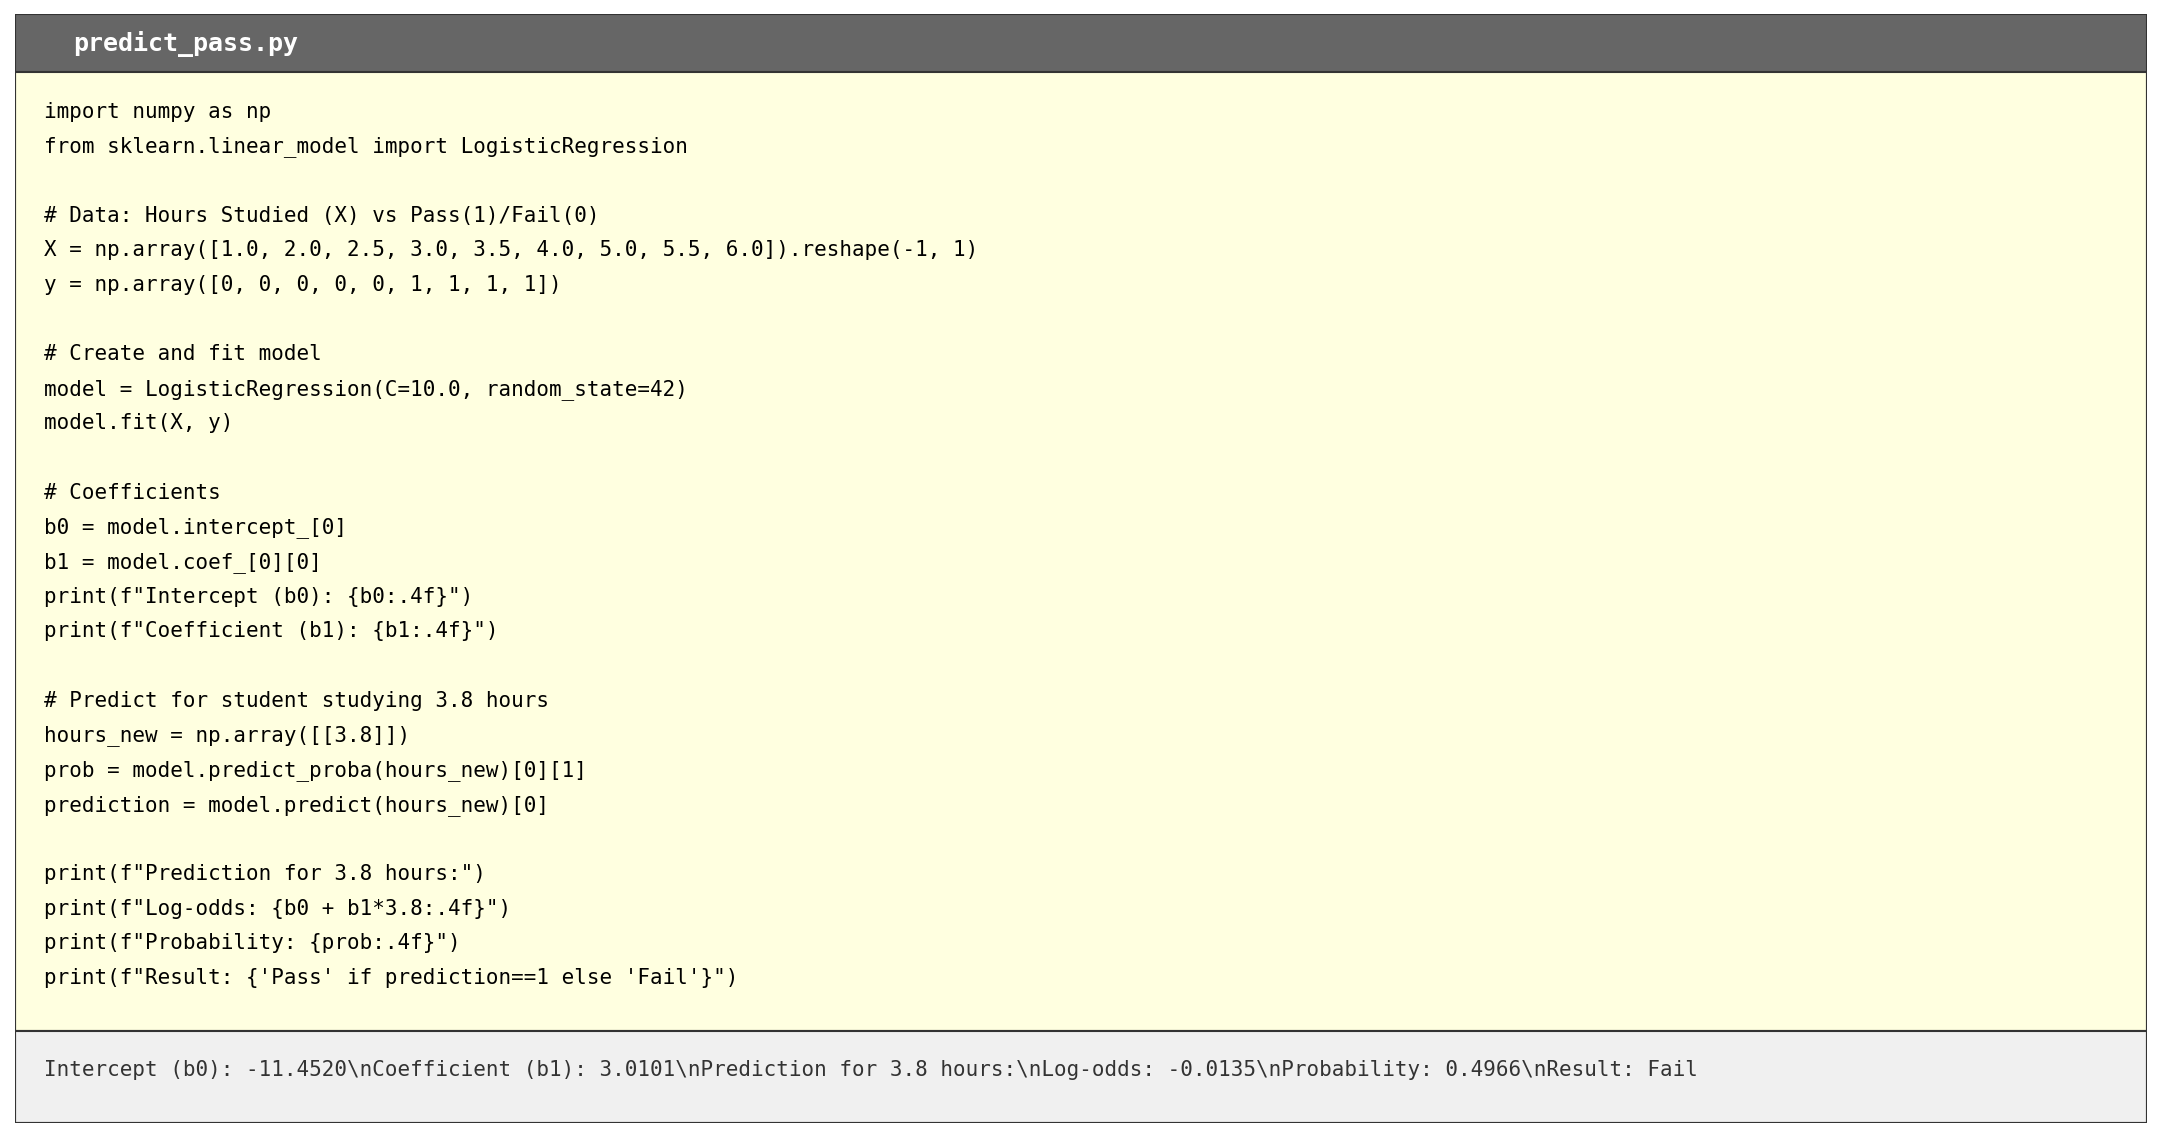
\includegraphics[width=1\textwidth]{CH3_ex1_combined.png}
	\caption{Python Code และผลลัพธ์การพยากรณ์การสอบผ่านจากชั่วโมงอ่านหนังสือ}
	\label{fig:ex1_pass}
\end{figure}

\subsubsection{กรณีศึกษาที่ 2: การประเมินความเสี่ยงทางการแพทย์ (ตัวแปรอิสระพหุคูณ)}
ในวิทยาการระบาดและการแพทย์ การประเมินความเสี่ยงต่อการเกิดโรค (Risk Assessment) มักต้องพิจารณาปัจจัยร่วมหลายประการ พิจารณาชุดข้อมูลตัวอย่างของผู้ป่วย 10 ราย โดยมีตัวแปรทำนายคือ อายุ (Age) และระดับคอเลสเตอรอล (Cholesterol) เพื่อทำนายสถานะการเกิดโรคหัวใจ (Disease Status) ดังตาราง \ref{T:data_heartattack}

\begin{table}[h]
\caption{ชุดข้อมูลตัวอย่างของผู้ป่วยสำหรับใช้การประเมินความเสี่ยงต่อการเกิดโรคหัวใจ}
\label{T:data_heartattack}
\centering
\begin{tabular}{|c|c|c|c|}
\hline
\textbf{Subject} & \textbf{Age (Years)} & \textbf{Cholesterol (mg/dL)} & \textbf{Disease Status (1=Yes, 0=No)} \\
\hline
1 & 25 & 180 & 0 \\
2 & 30 & 190 & 0 \\
3 & 45 & 220 & 1 \\
4 & 50 & 240 & 1 \\
5 & 60 & 260 & 1 \\
6 & 35 & 200 & 0 \\
7 & 40 & 210 & 0 \\
8 & 55 & 250 & 1 \\
9 & 65 & 280 & 1 \\
10 & 58 & 230 & 1 \\
\hline
\end{tabular}
\end{table}

\noindent
ผลการวิเคราะห์ด้วยการถดถอยโลจิสติคพหุคูณ (ภาพประกอบ \ref{fig:ex2_heart}) ได้สมการของ Log-odds (Logit) แสดงดังนี้
$$\ln\left(\frac{p}{1-p}\right) \approx -0.1394 + 6.9918(\text{Age}) - 1.3814(\text{Chol})$$
\textit{ข้อสังเกต: ค่าสัมประสิทธิ์ที่นำเสนอนี้เป็นค่าประมาณจากข้อมูลตัวอย่างเพื่อการสาธิตเท่านั้น}

\noindent
\textbf{โจทย์ปัญหา:} จงประเมินความเสี่ยงในการเป็นโรคหัวใจสำหรับผู้ป่วยที่มีอายุ 52 ปี และมีระดับคอเลสเตอรอล 235 mg/dL
\begin{enumerate}
	\item[] \textbf{ขั้นตอนที่ 1 การคำนวณค่าลอจิต}
	ด้วยการแทนค่าตัวแปรทั้งสองลงในสมการทำนาย ดังนี้
	\begin{eqnarray} \nonumber
		\hat{y} &=& -0.1394 + 6.9918(52) - 1.3814(235) \\  \nonumber
		&=& -0.1394 + 363.5736 - 324.6290 \\ \nonumber 
		 &=& 38.8052
	\end{eqnarray}
	
	\item[] \textbf{ขั้นตอนที่ 2 การคำนวณความน่าจะเป็น}
	$$ P(Y=1| x_1 = 52, x_2 = 235)= p = \frac{1}{1 + e^{-38.8052}} \approx 1.0$$
	
\end{enumerate}
\textbf{สรุปผล:} ตัวแบบบ่งชี้อย่างชัดเจนว่าผู้ป่วยรายนี้มีความเสี่ยงสูงมาก (เข้าใกล้ 100\%) ที่จะตรวจพบโรคหัวใจ ผลลัพธ์นี้สอดคล้องกับลักษณะของข้อมูลที่แสดงให้เห็นว่าผู้ที่มีอายุมากและระดับคอเลสเตอรอลสูงมีแนวโน้มที่จะเป็นกลุ่มเสี่ยง การวิเคราะห์เช่นนี้ช่วยให้แพทย์สามารถคัดกรองผู้ป่วยกลุ่มเสี่ยงเพื่อการดูแลอย่างใกล้ชิดได้

\begin{figure}[h]
	\centering
	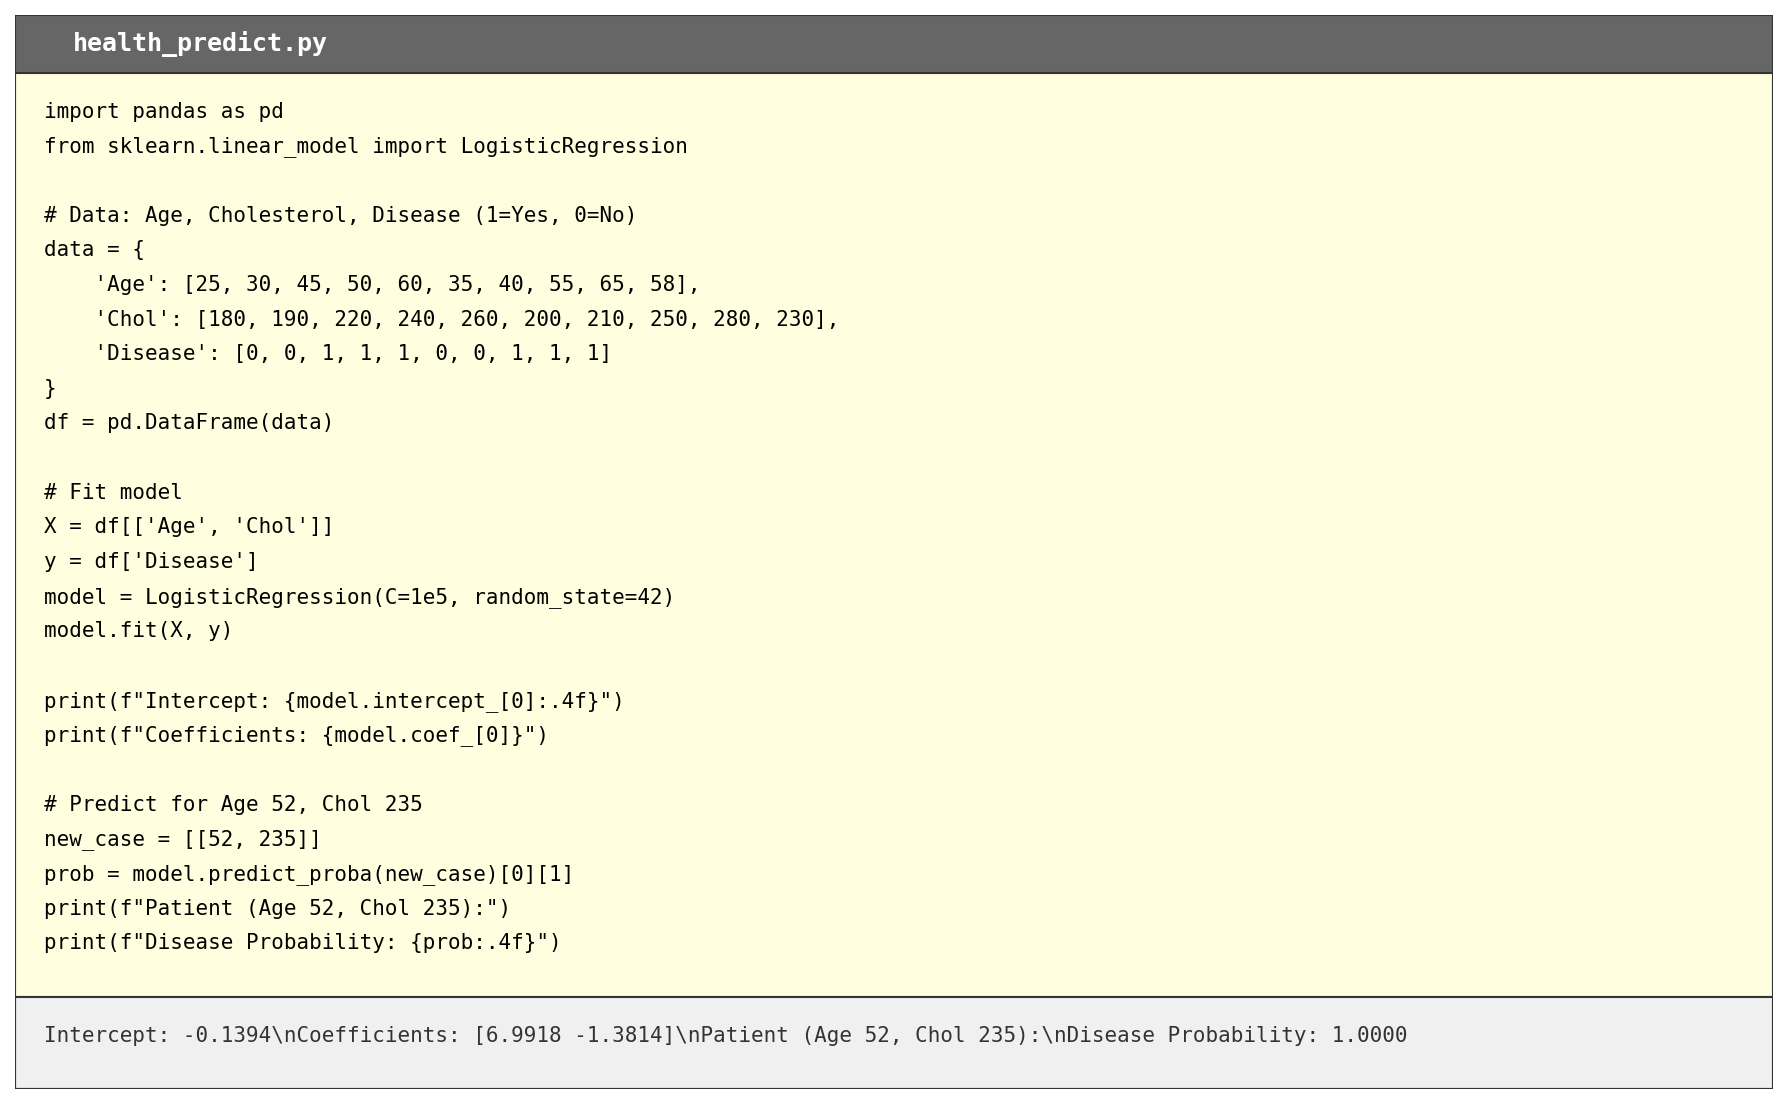
\includegraphics[width=1\textwidth]{CH3_ex2_combined.png}
	\caption{Python Code และการวิเคราะห์ความเสี่ยงโรคหัวใจด้วยตัวแปรพหุคูณ}
	\label{fig:ex2_heart}
\end{figure}

\subsection{แบบฝึกหัดท้ายบท (Assignments)}

จงวิเคราะห์ข้อมูลและสร้างตัวแบบถดถอยโลจิสติคสำหรับโจทย์ต่อไปนี้ พร้อมแสดงวิธีการคำนวณและผลลัพธ์จากโปรแกรม Python โดยแบ่งเป็นกรณีตัวแปรอิสระเดี่ยว (Simple Logistic Regression) และตัวแปรอิสระพหุคูณ (Multiple Logistic Regression)

\subsubsection*{ส่วนที่ 1: การถดถอยโลจิสติคแบบตัวแปรเดียว (Simple Logistic Regression)}

\paragraph{ข้อที่ 1 การเลื่อนตำแหน่งพนักงาน (Promotion Prediction):}  ฝ่ายทรัพยากรบุคคลต้องการทำนายโอกาสที่พนักงานจะได้เลื่อนตำแหน่ง (Promoted: 1=ได้, 0=ไม่ได้) โดยพิจารณาจากประสบการณ์ทำงาน (Experience) เพียงอย่างเดียว ข้อมูลพนักงาน 10 คนแสดงดังตาราง \ref{T:data_promotePrediced}

\begin{table}[h]
\caption{ชุดข้อมูลตัวอย่างสำหรับใช้ในการพิจารณาเลื่อนตำแหน่งจากประสบการณ์ทำงานของพนักงาน}
\label{T:data_promotePrediced}
\centering
\begin{tabular}{|c|c|c|c|c|c|c|c|c|c|c|}
\hline
\text{Exp (Yrs)} & 1 & 2 & 3 & 4 & 5 & 6 & 7 & 8 & 9 & 10 \\
\hline
\text{Promoted} & 0 & 0 & 0 & 0 & 1 & 0 & 1 & 1 & 1 & 1 \\
\hline
\end{tabular}
\end{table}

\noindent
\textbf{โจทย์ปัญหา:}
จงสร้างตัวแบบและทำนายโอกาสที่พนักงานที่มีประสบการณ์ 5.5 ปี จะได้รับการเลื่อนตำแหน่ง

\noindent
\textbf{วิธีทำ}

1. \textbf{การคำนวณค่า Logit} แสดงดังนี้
$$\hat{y} = -6.7243 + 1.2226(5.5) = -0.0000$$

โดยที่ $\hat{\beta}_0 \approx -6.7243$, $\hat{\beta}_1 \approx 1.2226$


2. \textbf{การคำนวณความน่าจะเป็น} แสดงดังนี้
$$P(Y=1| x=5.5)= p = \frac{1}{1 + e^{0.0000}}  = 0.5000$$
ดังนั้น พนักงานที่มีประสบการณ์ 5.5 ปี จะได้รับการเลื่อนตำแหน่งคิดเป็น 50\%

\begin{figure}[h!]
	\centering
	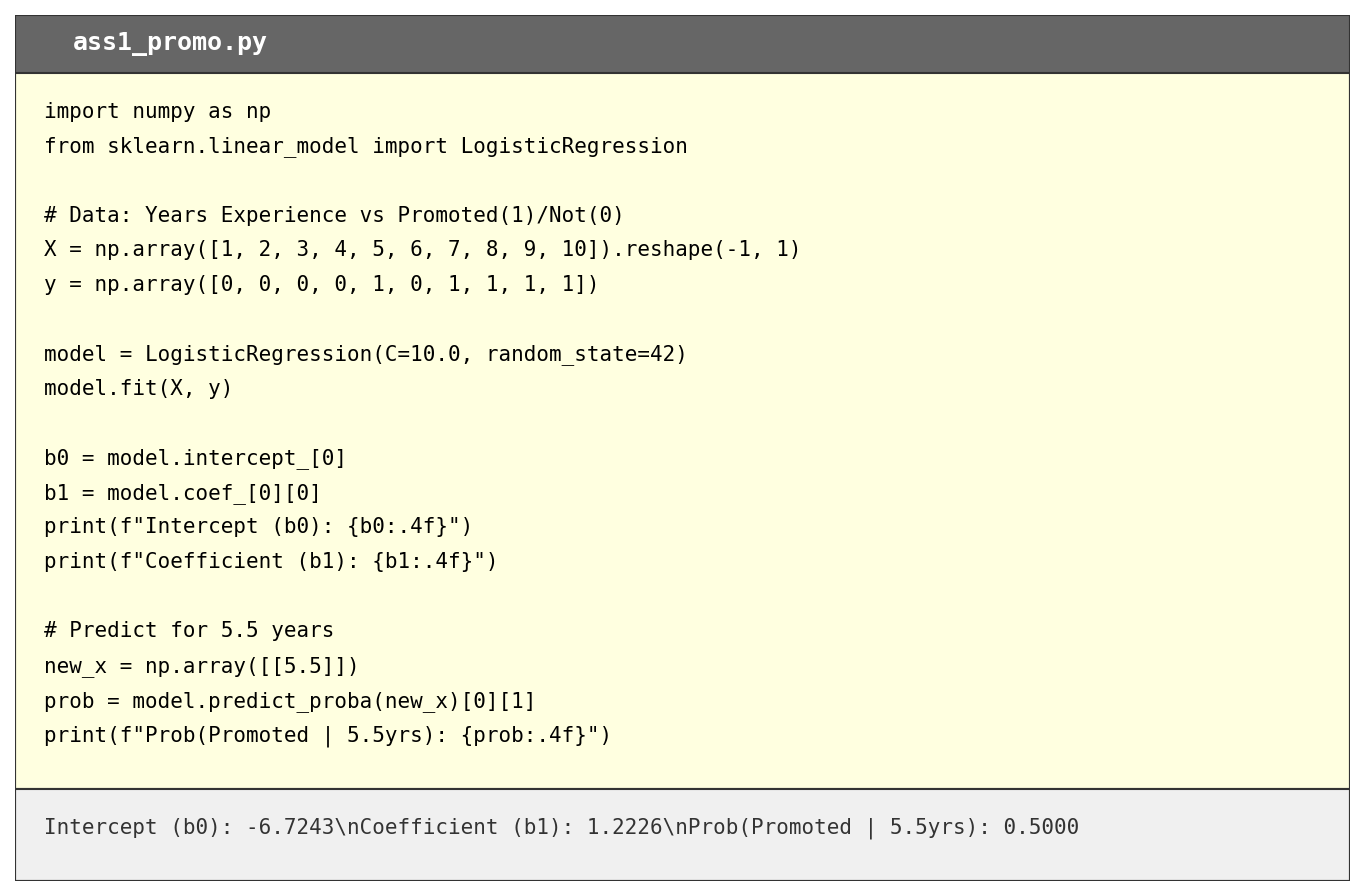
\includegraphics[width=1\textwidth]{CH3_ass1_combined.png}
	\caption{การวิเคราะห์การเลื่อนตำแหน่ง (ตัวแปรเดียว)}
\end{figure}

\paragraph{ข้อที่ 2 การทำนายความล้มเหลวของเครื่องจักร (Machine Failure):} วิศวกรต้องการตรวจสอบผลของอุณหภูมิ (Temperature) ต่อความล้มเหลวของเครื่องจักร (Failure: 1=เสีย, 0=ปกติ)
แสดงดังตาราง \ref{T:data_temp}

\begin{table}[h]
\caption{ชุดข้อมูลตัวอย่างสำหรับการทำนายความล้มเหลวของเครื่องจักร}
\label{T:data_temp}
\centering
\begin{tabular}{|c|c|c|c|c|c|c|c|c|c|c|}
\hline
\text{Temp ($^\circ$C)} & 50 & 55 & 60 & 65 & 70 & 75 & 80 & 85 & 90 & 95 \\
\hline
\text{Failure} & 0 & 0 & 0 & 0 & 0 & 1 & 0 & 1 & 1 & 1 \\
\hline
\end{tabular}
\end{table}

\noindent
\textbf{โจทย์ปัญหา:}
จงทำนายความน่าจะเป็นที่เครื่องจักรจะเสียหายเมื่ออุณหภูมิอยู่ที่ 72 $^\circ$C

\noindent
\textbf{วิธีทำ}


1. \textbf{การคำนวณค่า Logit} แสดงดังนี้
$$\hat{y} = -20.0434 + 0.2586(72) = -1.4242$$

โดยที่ $\hat{\beta}_0 \approx -20.0434$, $\hat{\beta}_1 \approx 0.2586$

2. \textbf{การคำนวณความน่าจะเป็น} แสดงดังนี้

$$P(Y=1| x=72)=p = \frac{1}{1 + e^{-1.4242}}\approx 0.1940$$

\begin{figure}[h!]
	\centering
	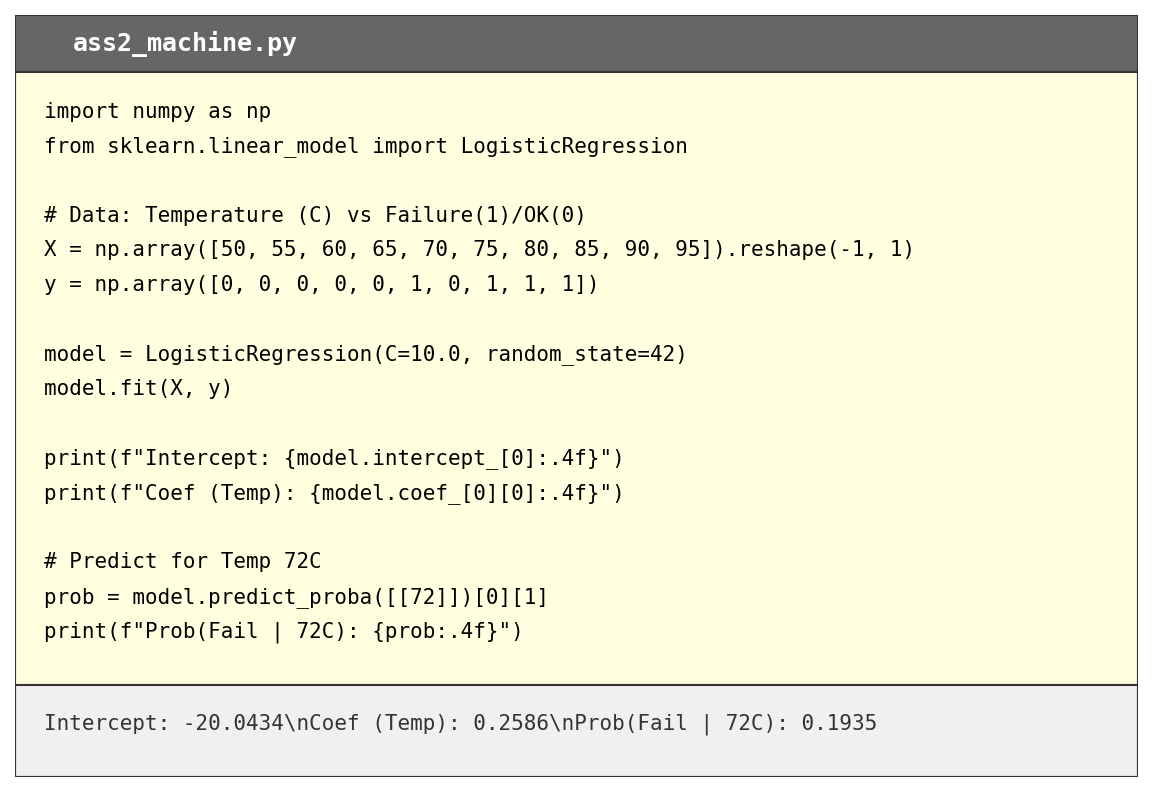
\includegraphics[width=1\textwidth]{CH3_ass2_combined.png}
	\caption{การวิเคราะห์ความล้มเหลวเครื่องจักร (ตัวแปรเดียว)}
\end{figure}

\subsubsection*{ส่วนที่ 2: การถดถอยโลจิสติคพหุคูณ (Multiple Logistic Regression)}

\paragraph{ข้อที่ 1 การวิเคราะห์พฤติกรรมการซื้อสินค้า (Customer Purchase):} การทำนายการตัดสินใจซื้อสินค้า (Buy: 1=ซื้อ) โดยใช้ตัวแปร \textbf{อายุ (Age)} และ \textbf{เงินเดือน (Salary)} แสดงดังตาราง \ref{T:data_heartattack}

\begin{table}[h]
\caption{ชุดข้อมูลตัวอย่างสำหรับใช้ทำนายการตัดสินใจซื้อสินค้าเพื่อวิเคราะห์พฤติกรรมของผู้บริโภค}
\label{T:data_custumer}
\centering
\begin{tabular}{|c|c|c||c|c|c|}
\hline
\text{Age} & \text{Salary} & \text{Buy} & \text{Age} & \text{Salary} & \text{Buy} \\
\hline
20 & 20,000 & 0 & 45 & 90,000 & 1 \\
25 & 25,000 & 0 & 50 & 40,000 & 0 \\
30 & 30,000 & 0 & 55 & 95,000 & 1 \\
35 & 80,000 & 1 & 22 & 22,000 & 0 \\
40 & 35,000 & 0 & 48 & 85,000 & 1 \\
\hline
\end{tabular}
\end{table}

\noindent
\textbf{โจทย์ปัญหา:}
จงทำนายโอกาสการซื้อของลูกค้าอายุ \textbf{42 ปี} และมีเงินเดือน \textbf{75,000 บาท}

\noindent
\textbf{วิธีทำ}

1. \textbf{สมการ Logit} แสดงดังนี้
$$\hat{y} \approx -0.0224 - 0.3942(\text{Age}) + 0.0003(\text{Salary})$$

2. \textbf{การแทนค่า} แสดงดังนี้
$$\hat{y} = -0.0224 - 16.5564 + 22.5000 = 5.9212$$

3. \textbf{การคำนวณความน่าจะเป็น} แสดงดังนี้
$$P(Y=1| \text{Age} = 42 , \text{Salary}= 75000 )= p = \frac{1}{1 + e^{-5.9212}} = 0.9973$$

\begin{figure}[h]
	\centering
	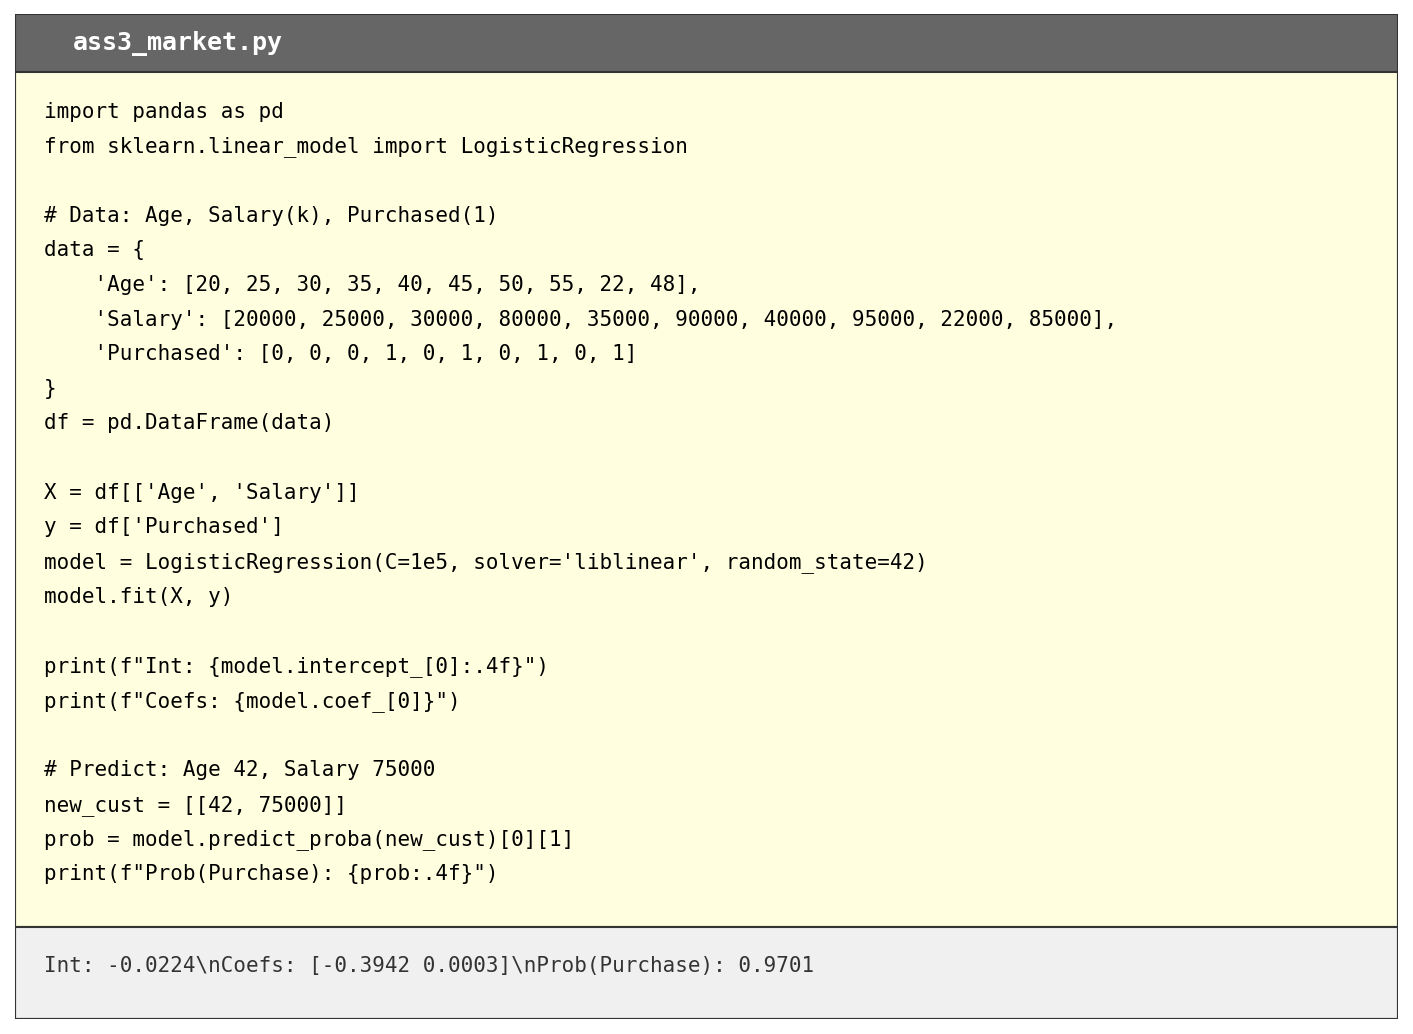
\includegraphics[width=1\textwidth]{CH3_ass3_combined.png}
	\caption{การวิเคราะห์การซื้อสินค้า (หลายตัวแปร)}
\end{figure}

\paragraph{ข้อที่ 4 การประเมินความเสี่ยงสินเชื่อ (Credit Scoring):} การทำนายการผิดนัดชำระหนี้ (Default=1) โดยใช้ 5 ตัวแปรอิสระ ได้แก่ คะแนนเครดิต (Score), รายได้ต่อปี (Income k\$), สัดส่วนหนี้ต่อรายได้ (DTI \%), ประสบการณ์ทำงาน (Emp Yrs), และ วงเงินกู้ (Loan k\$) รายละเอียดแสดงดังตาราง \ref{T:data_credit}

\begin{table}[h]
\caption{ชุดข้อมูลตัวอย่างสำหรับทำนายการผิดนัดชำระหนี้ด้วย 5 ตัวแปร}
\label{T:data_credit}
\centering
\begin{tabular}{|c|c|c|c|c|c||c|c|c|c|c|c|}
\hline
\text{Score} & \text{Inc} & \text{DTI} & \text{Emp} & \text{Loan} & \text{Def} & \text{Score} & \text{Inc} & \text{DTI} & \text{Emp} & \text{Loan} & \text{Def} \\
\hline
800 & 80 & 5 & 10 & 10 & 0 & 600 & 45 & 20 & 3 & 25 & 1 \\
780 & 75 & 8 & 9 & 15 & 0 & 550 & 40 & 25 & 2 & 30 & 1 \\
750 & 70 & 10 & 8 & 20 & 0 & 500 & 35 & 30 & 1 & 40 & 1 \\
700 & 60 & 12 & 6 & 12 & 0 & 450 & 30 & 35 & 0 & 45 & 1 \\
650 & 55 & 15 & 5 & 18 & 0 & 400 & 40 & 40 & 2 & 50 & 1 \\
\hline
\end{tabular}
\end{table}

\noindent
\textbf{โจทย์ปัญหา:}
จงประเมินความเสี่ยงของผู้กู้ที่มีข้อมูล ดังนี้ Score=\textbf{620}, Income=\textbf{50k}, DTI=\textbf{18\%}, Emp=\textbf{4 ปี}, Loan=\textbf{22k}

\noindent
\textbf{วิธีทำ}

1. \textbf{สมการ Logit} จาก Python แสดงดังนี้
\begin{align*}
\hat{y} &= 0.0057 - 0.0028(\text{Score}) - 0.3418(\text{Inc}) \\
&\quad + 0.4268(\text{DTI}) - 0.1023(\text{Emp}) + 0.5452(\text{Loan})
\end{align*}

โดยที่ $\hat{\beta}_0 \approx 0.0057$, $\hat{\beta}_{Score} \approx -0.0028$, $\hat{\beta}_{Inc} \approx -0.3418$, $\hat{\beta}_{DTI} \approx 0.4268$,

$\hat{\beta}_{Emp} \approx -0.1023$, $\hat{\beta}_{Loan} \approx 0.5452$

2. \textbf{การแทนค่า} แสดงดังนี้
\begin{align*}
\hat{y} &= 0.0057 - 0.0028(620) - 0.3418(50) + 0.4268(18) - 0.1023(4) + 0.5452(22) \\
&= 0.0057 - 1.7360 - 17.0900 + 7.6824 - 0.4092 + 11.9944 \\
&\approx 0.4473
\end{align*}

3. \textbf{การคำนวณความน่าจะเป็น} แสดงดังนี้
$$P(Y=1| (620, 50k, 18\%, 4, 22k) ) = \frac{1}{1 + e^{-0.4473}} \approx
ดังนั้นผู้กู้รายนี้มีความเสี่ยงผิดนัดชำระหนี้ประมาณ 61.00\%

\begin{figure}[h]
	\centering
	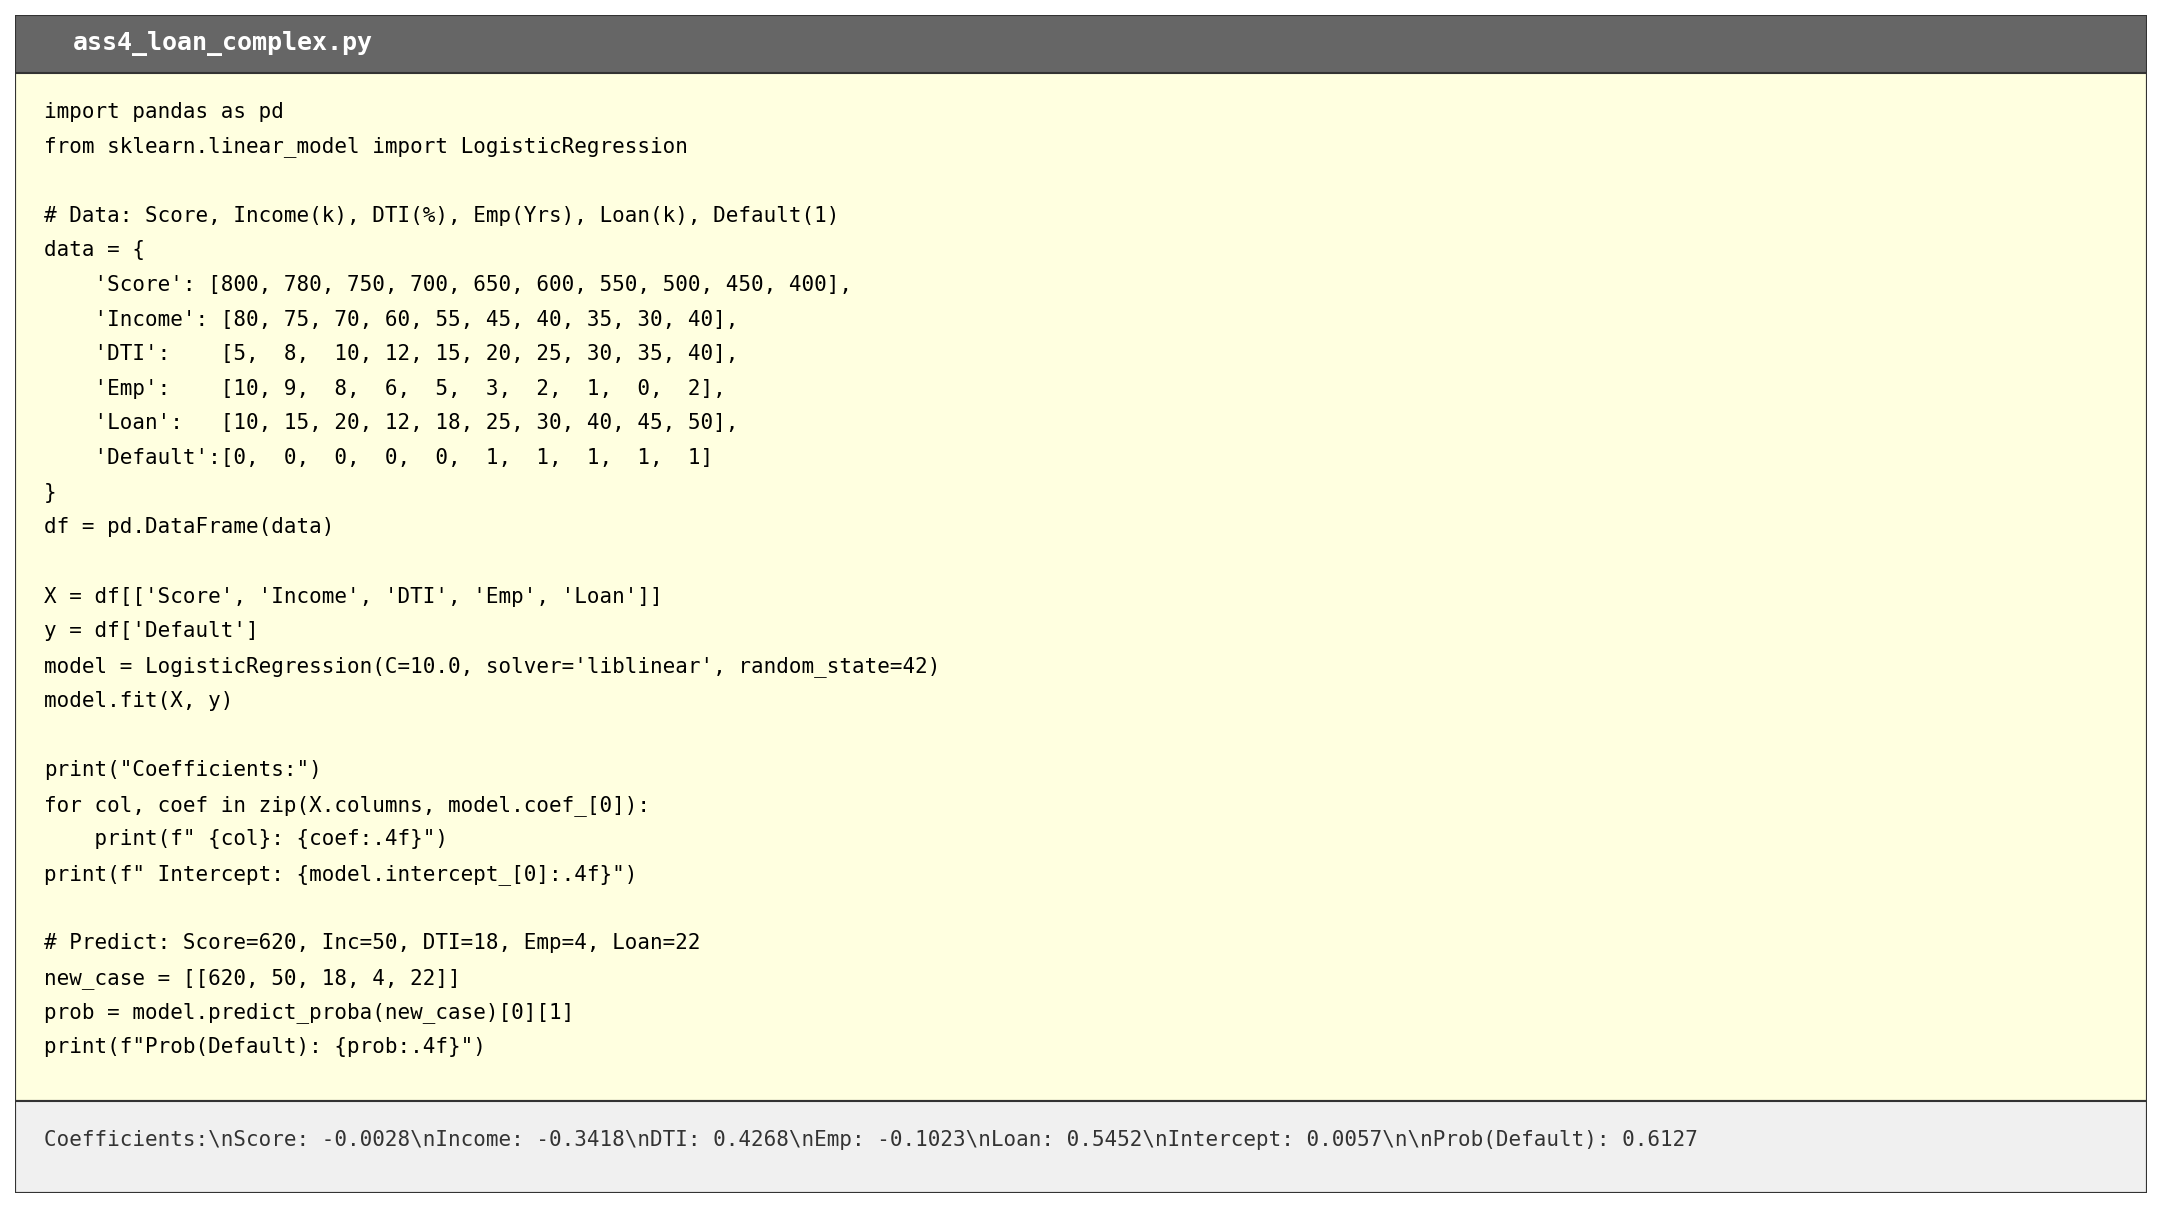
\includegraphics[width=1\textwidth]{CH3_ass4_combined.png}
	\caption{การประเมินความเสี่ยงสินเชื่อ (5 ตัวแปร)}
\end{figure}

\paragraph{ข้อที่ 5 การคลิกโฆษณาออนไลน์ (Ad Click Prediction):} การทำนายการคลิกโฆษณา (Click=1) โดยใช้ 5 ตัวแปรอิสระ ได้แก่ เวลาใช้งานอินเทอร์เน็ตต่อวัน (Usage นาที), อายุ (Age ปี), รายได้เฉลี่ยของพื้นที่ (Income k\$), เวลาที่ใช้ในเว็บไซต์ (Time นาที), และเพศ (Male: 1=ชาย, 0=หญิง) รายแสดง ดังตาราง \ref{T:data_Advertis}

\begin{table}[h]
\caption{ชุดข้อมูลตัวอย่างสำหรับใช้ในการการทำนายการคลิกโฆษณา}
\label{T:data_Advertis}
\centering
\begin{tabular}{|c|c|c|c|c|c||c|c|c|c|c|c|}
\hline
\text{Usage} & \text{Age} & \text{Inc} & \text{Time} & \text{Male} & \text{Click} & \text{Use} & \text{Age} & \text{Inc} & \text{Time} & \text{Male} & \text{Click} \\
\hline
30 & 50 & 30 & 10 & 1 & 1 & 80 & 25 & 60 & 35 & 0 & 0 \\
40 & 45 & 35 & 15 & 0 & 1 & 90 & 28 & 65 & 40 & 1 & 0 \\
50 & 40 & 40 & 20 & 1 & 1 & 100 & 22 & 70 & 45 & 0 & 0 \\
60 & 35 & 45 & 15 & 0 & 1 & 110 & 20 & 80 & 50 & 1 & 0 \\
70 & 30 & 55 & 30 & 1 & 0 & 120 & 18 & 85 & 55 & 0 & 0 \\
\hline
\end{tabular}
\end{table}

\noindent
\textbf{โจทย์ปัญหา:}
จงทำนายผู้ใช้ที่มีข้อมูล ดังนี้ Usage=\textbf{55 นาที}, Age=\textbf{38 ปี}, Income=\textbf{50k}, Time=\textbf{25 นาที}, เพศ=\textbf{ชาย}

\noindent
\textbf{วิธีทำ}

1. \textbf{สมการ Logit} จาก Python แสดงดังนี้
\begin{align*}
\hat{y} &= 0.0082 - 0.0375(\text{Use}) + 0.5457(\text{Age}) - 0.0991(\text{Inc}) \\
&\quad - 0.4584(\text{Time}) - 0.0312(\text{Male})
\end{align*}

โดยที่ $\hat{\beta}_0 \approx 0.0082$, $\hat{\beta}_{Usage} \approx -0.0375$, $\hat{\beta}_{Age} \approx 0.5457$, $\hat{\beta}_{Inc} \approx -0.0991$,

$\hat{\beta}_{Time} \approx -0.4584$, $\hat{\beta}_{Male} \approx -0.0312$

2. \textbf{การแทนค่า} แสดงดังนี้
\begin{align*}
\hat{y} &= 0.0082 - 0.0375(55) + 0.5457(38) - 0.0991(50) - 0.4584(25) - 0.0312(1) \\
&= 0.0082 - 2.0625 + 20.7366 - 4.9550 - 11.4600 - 0.0312 \\
&\approx 2.2384
\end{align*}

3. \textbf{การคำนวณความน่าจะเป็น} แสดงดังนี้
$$P(Y=1| (55,38, 50k, 25, 1) )  = \frac{1}{1 + e^{-2.2384}} \approx 0.9036$$
ดังนั้นโอกาสคลิกโฆษณาออนไลน์สูงถึงประมาณ 90.36\%

\begin{figure}[h]
	\centering
	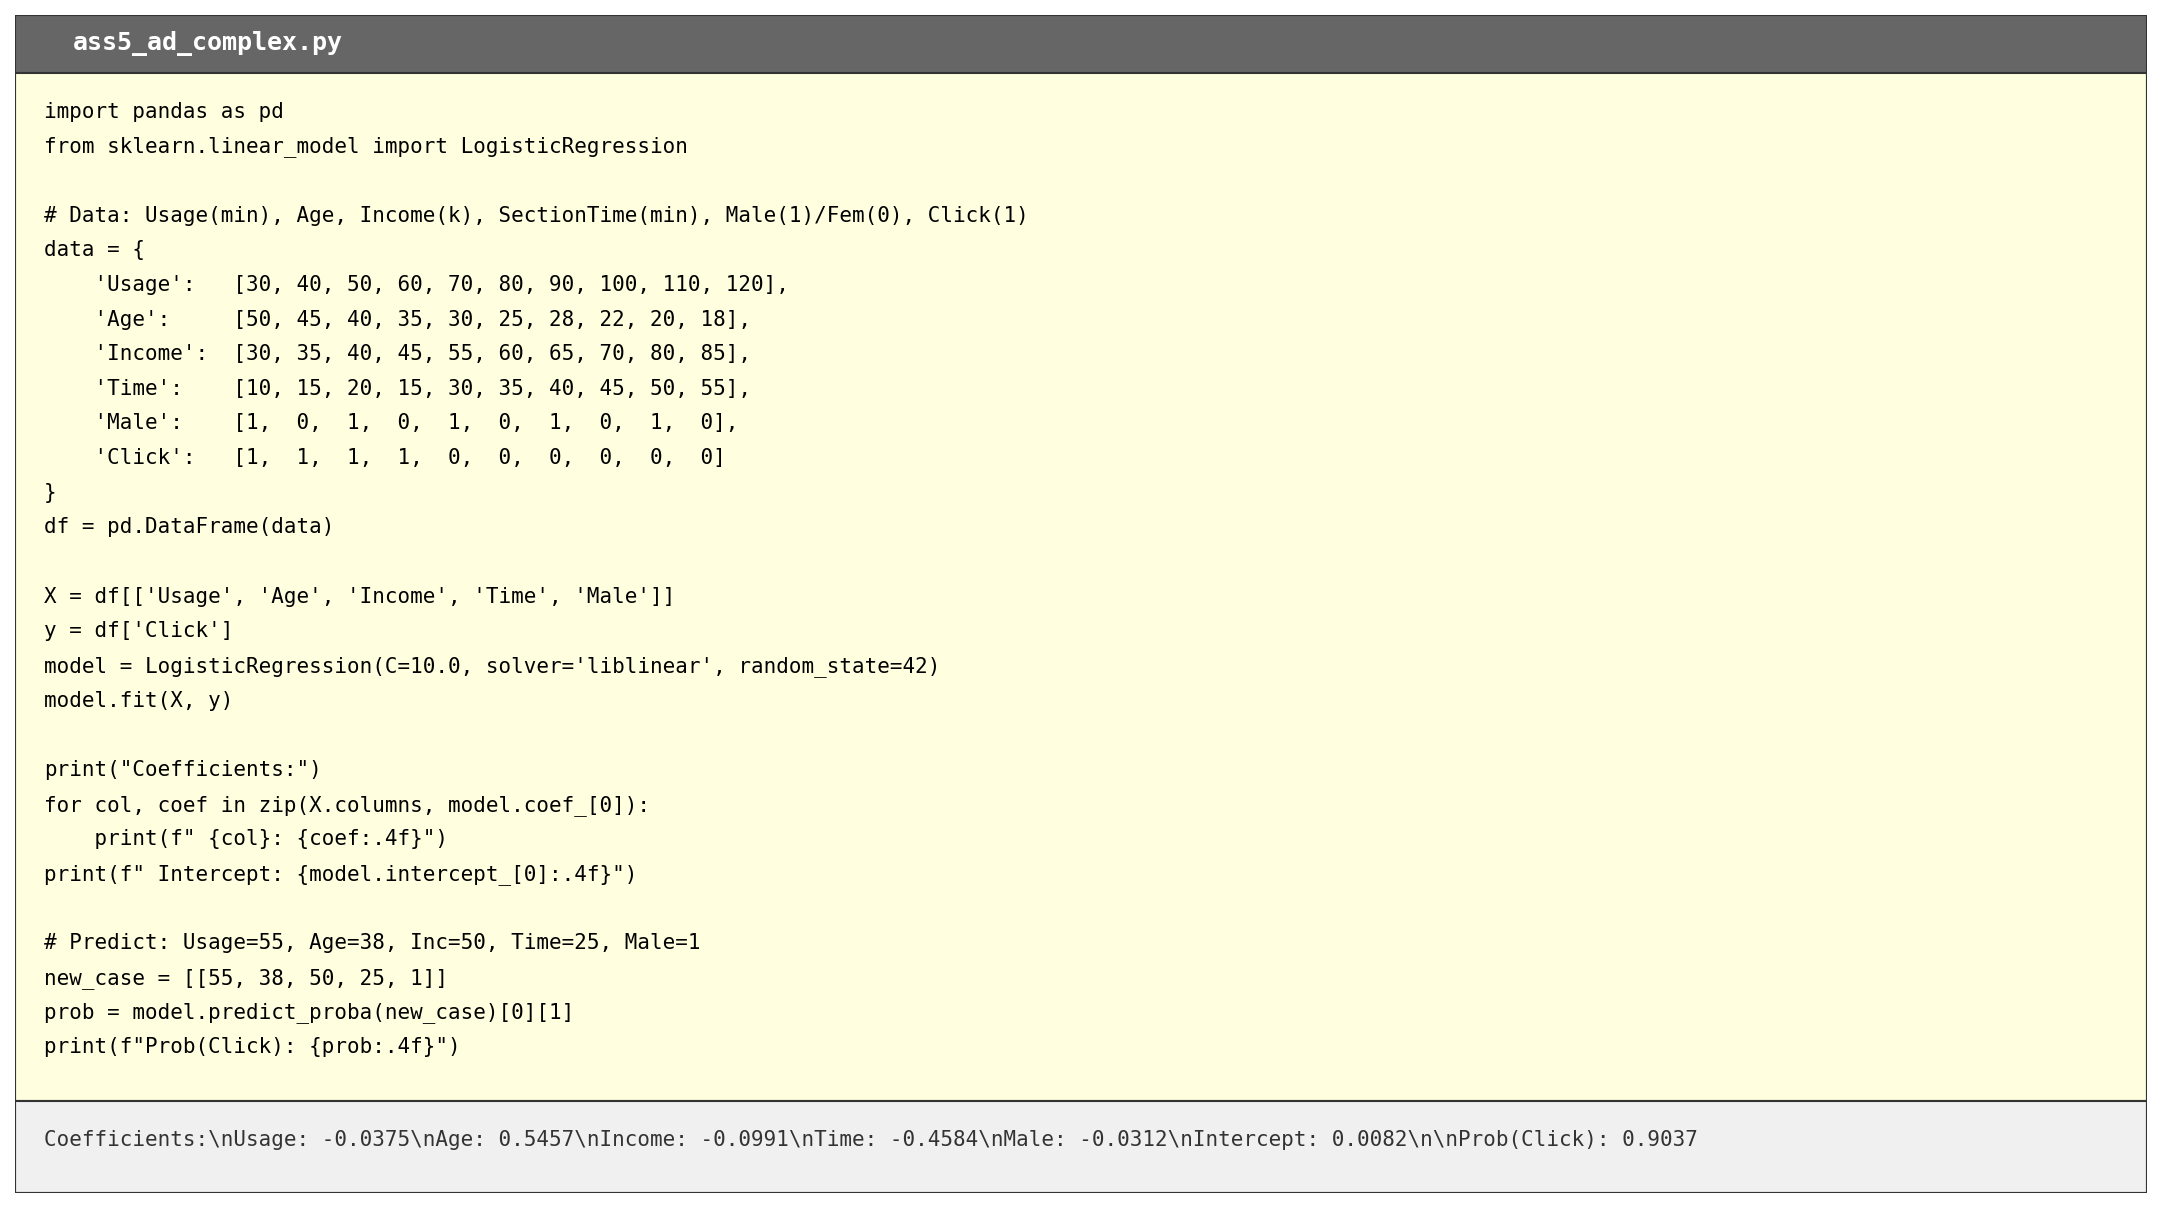
\includegraphics[width=1\textwidth]{CH3_ass5_combined.png}
	\caption{การทำนายการคลิกโฆษณา (5 ตัวแปร)}
\end{figure}


\newpage
\section{คุณสมบัติเด่นของการถดถอยโลจิสติค}
การถดถอยโลจิสติคมีข้อดีหลายประการเมื่อเทียบกับการถดถอยเชิงเส้นสำหรับข้อมูลเชิงคุณภาพ ดังนี้ 

\begin{myLimit}[]{คุณสมบัติเด่นของการถดถอยโลจิสติค}{}
	\begin{itemize}
		\item ค่าทำนายจะอยู่ในช่วง $[0, 1]$ เสมอ ทำให้สามารถตีความเป็นความน่าจะเป็นได้อย่างเหมาะสม ไม่มีปัญหาการทำนายค่านอกช่วงที่เป็นไปได้
		 
		\item ตัวแบบไม่ต้องอาศัยสมมติฐานเรื่องการกระจายแบบปกติของข้อผิดพลาด เนื่องจากอิงกับการกระจายแบบทวินาม (Binomial Distribution) ซึ่งเหมาะสมกับลักษณะของข้อมูลเชิงคุณภาพแบบทวิภาค
		
		\item การถดถอยโลจิสติคมีความทนทานต่อข้อมูลผิดปกติ (Outliers) มากกว่าการถดถอยเชิงเส้น เนื่องจากการใช้ฟังก์ชันซิกมอยด์ทำให้ผลกระทบของค่าสุดโต่งถูกลดทอนลง 
		
		
		\item ตัวแบบการถดถอยโลจิสติคสามารถขยายไปสู่รูปแบบที่ซับซ้อนขึ้น เช่น การถดถอยโลจิสติคแบบพหุนาม (Multinomial Logistic Regression) หรือการถดถอยโลจิสติคแบบลำดับ (Ordinal Logistic Regression) ได้อย่างธรรมชาติ
	\end{itemize}
\end{myLimit}

\section{หลักการของการประมาณค่าแบบภาวะน่าจะเป็นสูงสุด}

การประมาณค่าพารามิเตอร์ในแบบจำลองการถดถอยโลจิสติคแตกต่างจากการถดถอยเชิงเส้นอย่างพื้นฐาน เนื่องจากลักษณะของตัวแปรตามที่เป็นตัวแปรเชิงคุณภาพทำให้ไม่สามารถใช้วิธี Ordinary Least Squares (OLS) ได้อย่างมีประสิทธิภาพ วิธีการที่เหมาะสมและได้รับการยอมรับอย่างกว้างขวางคือการประมาณค่าแบบภาวะน่าจะเป็นสูงสุด (Maximum Likelihood Estimation: MLE) ซึ่งได้รับการพัฒนาโดย Ronald A. Fisher ในช่วงต้นศตวรรษที่ 20 และได้รับการขยายแนวคิดสำหรับแบบจำลองเชิงเส้นทั่วไปในภายหลัง

หลักการพื้นฐานของ MLE อยู่บนสมมติฐานที่ว่าข้อมูลที่เราสังเกตได้นั้นเป็นข้อมูลที่มีความน่าจะเป็นสูงสุดที่จะเกิดขึ้นภายใต้แบบจำลองที่กำหนด กล่าวอีกนัยหนึ่ง ค่าพารามิเตอร์ที่ดีที่สุดคือค่าที่ทำให้ข้อมูลที่สังเกตได้มีความน่าจะเป็นสูงสุด แนวคิดนี้มีความสมเหตุสมผลทั้งในแง่ของสัญชาตญาณและรากฐานทางคณิตศาสตร์ เนื่องจากหากแบบจำลองสะท้อนความเป็นจริงได้อย่างถูกต้อง ข้อมูลที่เราสังเกตได้ควรจะเป็นข้อมูลที่มีความน่าจะเป็นสูงในการเกิดขึ้น

%สำหรับการถดถอยโลจิสติคแบบทวิภาค สมมติว่าเรามีข้อมูล $\{(y_i, \mathbf{x}_i)\}_{i=1}^n$ โดยที่ $y_i \in \{0, 1\}$ เป็นตัวแปรตามและ $\mathbf{x}_i = (1, x_{i1}, x_{i2}, \ldots, x_{ki})'$ เป็นเวกเตอร์ของตัวแปรอิสระรวมทั้งค่าคงที่ การสังเกตแต่ละครั้งสามารถอธิบายได้ด้วยการทดลองแบบเบอร์นูลลี (Bernoulli Trial) ซึ่งมีความน่าจะเป็น $p_i = P(Y_i = 1|\mathbf{x}_i) = \frac{1}{1 + \exp(-\mathbf{X}^{T} \boldsymbol{\beta})}$ สำหรับการสังเกตที่ $i$ ลักษณะของการกระจายความน่าจะเป็นนี้ทำให้การใช้ MLE เป็นทางเลือกที่เหมาะสมและให้ผลลัพธ์ที่มีคุณสมบัติทางสถิติที่ดี


\subsubsection{การสร้างฟังก์ชันภาวะความน่าจะเป็น}

การสร้างฟังก์ชันภาวะความน่าจะเป็น (Likelihood Function) สำหรับการถดถอยโลจิสติคเริ่มจากการพิจารณาความน่าจะเป็นของการสังเกตแต่ละครั้ง สำหรับการสังเกตที่ $i$ ซึ่งสอดคล้องกับการแจกแจงแบร์นูลล์ลี (Bernoulli distribution) โดยที่ฟังก์ชันความหนาแน่นของความน่าจะเป็น (Probability Mass Function: pmf) ของการแจกจงดังกล่าว คือ 

$$P(Y=y_i)= f(y_i|\mathbf{x}_i, \boldsymbol{\beta}) = p_i^{y_i}(1-p_i)^{1-y_i}$$

\noindent
โดยที่ $\sum_{y_i=0}^{1} f(y_i|\mathbf{x}_i, \boldsymbol{\beta}) = (1-p_i) + p_i = 1$ นอกจากนี้ภายใต้สมมติฐานความเป็นอิสระและอยู่ภายใต้การแจกแจงเดียวกันจะได้ว่าฟังก์ชันภาวะความน่าจะเป็นสำหรับข้อมูลทั้งหมดจะเป็นผลคูณของความน่าจะเป็นของการสังเกตแต่ละครั้ง กล่าวคือ

\begin{eqnarray} \nonumber
	L(\boldsymbol{\beta}) = \prod_{i=1}^{n} f(y_i|\mathbf{x}_i, \boldsymbol{\beta}) 
	&=& \prod_{i=1}^{n} p_i^{y_i}(1-p_i)^{1-y_i} \\ \nonumber
	&=& \prod_{i=1}^{n} \left[\frac{\exp(\mathbf{X}^{T} \boldsymbol{\beta})}{1 + \exp(\mathbf{X}^{T} \boldsymbol{\beta})}\right]^{y_i} \left[\frac{1}{1 + \exp(\mathbf{X}^{T} \boldsymbol{\beta})}\right]^{1-y_i} \\ \nonumber
	&=& \left[\frac{\exp(\mathbf{X}^{T} \boldsymbol{\beta})}{1 + \exp(\mathbf{X}^{T} \boldsymbol{\beta})}\right]^{\sum_{i=1}^{n}y_i} \left[\frac{1}{1 + \exp(\mathbf{X}^{T} \boldsymbol{\beta})}\right]^{\sum_{i=1}^{n}1-y_i} \\ \nonumber
	&=& \frac{[\exp(\mathbf{X}^{T} \boldsymbol{\beta})]^{\sum_{i=1}^{n}y_i}}{[1 + \exp(\mathbf{X}^{T} \boldsymbol{\beta})]^{\sum_{i=1}^{n}(1-y_i) + \sum_{i=1}^{n}y_i}} 
\end{eqnarray}

\noindent
จากข้างต้นจะได้ ฟังก์ชันล็อคภาวะน่าจะเป็นดังนี้

\begin{eqnarray} \nonumber
	\ell(\boldsymbol{\beta}) = \ln L(\boldsymbol{\beta}) 
	&=& \ln \left[\frac{[\exp(\mathbf{X}^{T} \boldsymbol{\beta})]^{\sum_{i=1}^{n}y_i}}{[1 + \exp(\mathbf{X}^{T} \boldsymbol{\beta})]^{\sum_{i=1}^{n}1}} \right] \\ \nonumber
	&=& \sum_{i=1}^{n} \left[\ln(\exp(y_i \mathbf{X}^{T} \boldsymbol{\beta})) - \ln(1 + \exp(\mathbf{X}^{T} \boldsymbol{\beta}))\right] \\ \nonumber
	&=& \sum_{i=1}^{n} [y_i \mathbf{X}^{T} \boldsymbol{\beta} - \ln(1 + \exp(\mathbf{X}^{T} \boldsymbol{\beta}))] \\ \nonumber
	&=& \sum_{i=1}^{n} [y_i \ln(p_i) + (1-y_i) \ln(1-p_i)]
\end{eqnarray}

\noindent
สำหรับ $\ell(\boldsymbol{\beta}) = \sum_{i=1}^{n} [y_i \mathbf{X}^{T} \boldsymbol{\beta} - \ln(1 + \exp(\mathbf{X}^{T} \boldsymbol{\beta}))]$ คือรูปแบบ Canonical ของฟังก์ชันลอการิทึมความน่าจะเป็นสำหรับการถดถอยโลจิสติค โดยที่ $\ln(p_i)$ และ $\ln(1-p_i)$ สามารถอยู่ในรูปดังนี้

\begin{eqnarray} \nonumber
	\ln(p_i) &=& \ln\left(\frac{\exp(\mathbf{X}^{T} \boldsymbol{\beta})}{1 + \exp(\mathbf{X}^{T} \boldsymbol{\beta})}\right) = \ln(\exp(\mathbf{X}^{T} \boldsymbol{\beta})) - \ln(1 + \exp(\mathbf{X}^{T} \boldsymbol{\beta})) = \mathbf{X}^{T} \boldsymbol{\beta} - \ln(1 + \exp(\mathbf{X}^{T} \boldsymbol{\beta})) \\ \nonumber
	\ln(1-p_i) &=& \ln\left(\frac{1}{1 + \exp(\mathbf{X}^{T} \boldsymbol{\beta})}\right) = \ln(1) - \ln(1 + \exp(\mathbf{X}^{T} \boldsymbol{\beta})) = -\ln(1 + \exp(\mathbf{X}^{T} \boldsymbol{\beta}))
\end{eqnarray}

\noindent 
สำหรับการพิสูจน์ย้อนกลับโดยการแทนค่าเหล่านี้ จะได้ว่า

\begin{eqnarray} \nonumber
	y_i \ln(p_i) + (1-y_i) \ln(1-p_i) &=& y_i [\mathbf{X}^{T} \boldsymbol{\beta} - \ln(1 + \exp(\mathbf{X}^{T} \boldsymbol{\beta}))] + (1-y_i) [-\ln(1 + \exp(\mathbf{X}^{T} \boldsymbol{\beta}))] \\ \nonumber
	&=& y_i \mathbf{X}^{T} \boldsymbol{\beta} - y_i \ln(1 + \exp(\mathbf{X}^{T} \boldsymbol{\beta})) - (1-y_i) \ln(1 + \exp(\mathbf{X}^{T} \boldsymbol{\beta})) \\ \nonumber
	&=& y_i \mathbf{X}^{T} \boldsymbol{\beta} - [y_i + (1-y_i)] \ln(1 + \exp(\mathbf{X}^{T} \boldsymbol{\beta})) \\ \nonumber
	&=& y_i \mathbf{X}^{T} \boldsymbol{\beta} - \ln(1 + \exp(\mathbf{X}^{T} \boldsymbol{\beta}))
\end{eqnarray}


\subsubsection{การพิสูจน์การหาอนุพันธ์อันดับที่หนึ่ง}

การหาอนุพันธ์อันดับที่หนึ่งของฟังก์ชันล็อคภาวะน่าจะเป็นเทียบกับพารามิเตอร์ $\beta_k$ นั้นมีเกี่ยวข้องกับการหาอนุพันธ์ของฟังก์ชันผสม เริ่มจากฟังก์ชันลอการิทึมความน่าจะเป็นในรูป Canonical คือ

$$\ell(\boldsymbol{\beta}) = \sum_{i=1}^{n} [y_i \mathbf{X}^{T} \boldsymbol{\beta} - \ln(1 + \exp(\mathbf{X}^{T} \boldsymbol{\beta}))]$$

สำหรับการหาอนุพันธ์ต่อ $\beta_k$ จะได้ 

\begin{eqnarray} \nonumber
	\frac{\partial \ell(\boldsymbol{\beta})}{\partial \beta_k}
	&=& \sum_{i=1}^{n} \left[\frac{\partial}{\partial \beta_k}(y_i \mathbf{X}^{T} \boldsymbol{\beta}) - \frac{\partial}{\partial \beta_k} \ln(1 + \exp(\mathbf{X}^{T} \boldsymbol{\beta}))\right] ; \mathbf{X}^{T} \boldsymbol{\beta} = \sum_{k=0}^{p} \beta_k x_{ki}  \\ \nonumber
	&=& \sum_{i=1}^{n} \left[ y_i \frac{\partial}{\partial \beta_k}\left(\sum_{k=0}^{p} \beta_k x_{ki}\right) - \frac{\partial}{\partial \beta_k} \ln(1 + \exp(\mathbf{X}^{T} \boldsymbol{\beta})) \right]  \\ \nonumber
	&=&  \sum_{i=1}^{n} \left[ y_i x_{ki} - \frac{1}{1 + \exp(\mathbf{X}^{T} \boldsymbol{\beta})}\frac{\partial}{\partial \beta_k} [1 + \exp(\mathbf{X}^{T} \boldsymbol{\beta})]\right] \\ \nonumber
	&=&  \sum_{i=1}^{n} \left[ y_i x_{ki} - \frac{\exp(\mathbf{X}^{T} \boldsymbol{\beta})}{1 + \exp(\mathbf{X}^{T} \boldsymbol{\beta})}\frac{\partial}{\partial \beta_k}\left(\sum_{k=0}^{p} \beta_k x_{ki}\right)\right] \\ \nonumber
	&=&  \sum_{i=1}^{n} (y_i x_{ki} - p_i x_{ki})  \\ \nonumber  
	&=& \sum_{i=1}^{n} x_{ki}(y_i - p_i)
\end{eqnarray}

\noindent
โดยที่ 
$$\frac{\partial \ell(\beta_k)}{\partial \beta_k} = \left\{\begin{matrix}
	1 &;   k=j\\
	0 &;   k\neq j  \\
\end{matrix}\right. $$

\noindent
นอกจากนี้การพิสูจน์อนุพันธ์ของพจน์ที่สอง $\frac{\partial}{\partial \beta_k} \ln(1 + \exp(\mathbf{X}^{T} \boldsymbol{\beta}))$ ต้องใช้กฎลูกโซ่ (Chain Rule) กำหนดให้ $u = \mathbf{X}^{T} \boldsymbol{\beta}$ จะได้ว่า 

\begin{eqnarray} \nonumber
	\frac{\partial}{\partial \beta_k} \ln(1 + \exp(u)) &=& \frac{1}{1 + \exp(u)} \cdot \frac{\partial}{\partial \beta_k}(1 + \exp(u)) \\ \nonumber
	&=& \frac{1}{1 + \exp(u)} \cdot \exp(u) \cdot \frac{\partial u}{\partial \beta_k}
\end{eqnarray}

\noindent
เนื่องจาก $\frac{\partial u}{\partial \beta_k} = \frac{\partial}{\partial \beta_k}(\mathbf{X}^{T} \boldsymbol{\beta}) = x_{ki}$ จะได้ว่า

$$\frac{\partial}{\partial \beta_k} \ln(1 + \exp(\mathbf{X}^{T} \boldsymbol{\beta})) = \frac{\exp(\mathbf{X}^{T} \boldsymbol{\beta})}{1 + \exp(\mathbf{X}^{T} \boldsymbol{\beta})} \cdot x_{ki} = p_i x_{ki}$$


จากข้างต้นจะได้ว่า $\frac{\partial \ell(\boldsymbol{\beta})}{\partial \beta_k}  = \sum_{i=1}^{n} x_{ki}(y_i - p_i)$ คือฟังก์ชันคะแนน (Score Function) สำหรับพารามิเตอร์ $\beta_k$ การพิสูจน์ความถูกต้องของผลลัพธ์นี้สามารถทำได้โดยการตรวจสอบมิติ เนื่องจาก $y_i$ และ $p_i$ ต่างก็เป็นสเกลาร์ และ $x_{ki}$ เป็นองค์ประกอบของเมทริกซ์คุณลักษณะ ผลคูณ $x_{ki}(y_i - p_i)$ จึงมีมิติเดียวกับ $\beta_k$ ซึ่งสอดคล้องกับการเป็นอนุพันธ์

\subsubsection{การแปลงสู่รูปแบบเวกเตอร์และเมทริกซ์ (Vectorization)}

ในการประมวลผลด้วยคอมพิวเตอร์หรืออัลกอริทึมการบันทึกค่าเหมาะสมที่สุด (Optimization) เช่น Adam หรือ Gradient Descent เรานิยมใช้รูปแบบเมทริกซ์เพื่อความรวดเร็วและกระชับ จากอนุพันธ์ย่อยของฟังก์ชันลอการิทึมความน่าจะเป็น ($\ell$) สามารถเขียนในรูปของเวกเตอร์เกรเดียนต์ $\nabla \ell(\boldsymbol{\beta})$ ได้ดังนี้:

$$ \nabla \ell(\boldsymbol{\beta}) = \begin{bmatrix} \frac{\partial \ell}{\partial \beta_0} \\ \frac{\partial \ell}{\partial \beta_1} \\ \vdots \\ \frac{\partial \ell}{\partial \beta_p} \end{bmatrix} = \begin{bmatrix} \sum x_{0i}(y_i - p_i) \\ \sum x_{1i}(y_i - p_i) \\ \vdots \\ \sum x_{pi}(y_i - p_i) \end{bmatrix} = \mathbf{X}^T (\mathbf{y} - \mathbf{p}) $$

อย่างไรก็ตาม ในบริบทของการหาค่าเหมาะสมที่สุด เรามักกำหนดฟังก์ชันค่าสูญเสีย (Loss Function) เป็นฟังก์ชันลอการิทึมความน่าจะเป็นแบบลบ (Negative Log-Likelihood: NLL) เพื่อเปลี่ยนปัญหาจากการหาค่าสูงสุด (Maximize) เป็นการหาค่าต่ำสุด (Minimize) ดังนี้:
$$ J(\boldsymbol{\beta}) = -\ell(\boldsymbol{\beta}) $$

ดังนั้น เกรเดียนต์ $\mathbf{g}$ ที่ใช้ในอัลกอริทึม Adam (ตามที่ปรากฏในกรณีศึกษาที่ 2) จึงมีค่าเป็นอนุพันธ์ของ $J(\boldsymbol{\beta})$ ซึ่งสลับเครื่องหมายจาก $\nabla \ell(\boldsymbol{\beta})$ :
\begin{equation}
    \mathbf{g} = \nabla J(\boldsymbol{\beta}) = -\nabla \ell(\boldsymbol{\beta}) = -\mathbf{X}^T (\mathbf{y} - \mathbf{p}) = \mathbf{X}^T (\mathbf{p} - \mathbf{y})
    \label{eq:vector_gradient}
\end{equation}

รูปแบบ $\mathbf{g} = \mathbf{X}^T(\mathbf{p} - \mathbf{y})$ นี้คือที่มาทางทฤษฎีที่เชื่อมโยงระหว่างหลักการภาวะน่าจะเป็นสูงสุดและขั้นตอนการคำนวณทางโปรแกรม ซึ่งช่วยให้เราสามารถคำนวณเกรเดียนต์ของพารามิเตอร์ทุกตัวได้พร้อมกันด้วยการคูณเมทริกซ์เพียงครั้งเดียว

\subsubsection{การพิสูจน์การหาอนุพันธ์อันดับที่สอง}
การหาอนุพันธ์อันดับที่สองของของฟังก์ชันล็อคภาวะน่าจะเป็นเทียบกับพารามิเตอร์ $\beta_k$ ต่อจากฟังก์ชันคะแนนที่ได้จากขั้นตอนก่อนหน้า 

$$S_j(\boldsymbol{\beta}) = \frac{\partial \ell(\boldsymbol{\beta})}{\partial \beta_k} = \sum_{i=1}^{n} x_{ki}(y_i - p_i)$$ โดยเริ่มจาก

\begin{eqnarray} \nonumber
	\frac{\partial S_j(\boldsymbol{\beta})}{\partial \beta_k} = \frac{\partial^2 \ell(\boldsymbol{\beta})}{\partial \beta_k \partial \beta_k} &=& \sum_{i=1}^{n} x_{ki} \frac{\partial}{\partial \beta_k}(y_i - p_i)\hspace{0.5cm}; y_i\hspace{0.2cm}\text{เป็นค่าคงที่}  \\ \nonumber
	&=& \sum_{i=1}^{n} x_{ki} \left[-\frac{\partial p_i}{\partial \beta_k}\right] \\ \nonumber
	&=& -\sum_{i=1}^{n} x_{ki} \left[p_i(1-p_i) x_{ki}\right]  \\ \nonumber
	&=&-\sum_{i=1}^{n} x_{ki} p_i(1-p_i) \\ \nonumber
\end{eqnarray}

\noindent
การพิสูจน์การหาอนุพันธ์ของ $p_i$ เทียบกับ $\beta_k$ ต้องอาศัยการใช้กฎลูกโซ่กับฟังก์ชันซิกมอยด์ กำหนดให้ 

\begin{eqnarray} \nonumber
	u &=& \mathbf{X}^{T} \boldsymbol{\beta} \\ \nonumber
	p_i = \sigma(u) &=&  \frac{1}{1 + \exp(-u)}
\end{eqnarray}
\noindent
การหาอนุพันธ์ของฟังก์ชันซิกมอยด์ จะได้ว่า


$$\frac{d\sigma(u)}{du} = \frac{d}{du}\left(\frac{1}{1 + \exp(-u)}\right) = \frac{d}{du}(1 + \exp(-u))^{-1} = -(1 + \exp(-u))^{-2} \cdot (-\exp(-u)) = \frac{\exp(-u)}{(1 + \exp(-u))^2}$$ 

\noindent
จากนั้นการแปลงให้อยู่ในรูป $p_i$ จะได้ว่า 

$$\frac{d\sigma(u)}{du} = \frac{\exp(-u)}{(1 + \exp(-u))^2} = \frac{1}{1 + \exp(-u)} \cdot \frac{\exp(-u)}{1 + \exp(-u)} = p_i \cdot (1-p_i)$$

\noindent
จากการใช้กฎลูกโซ่  จะได้ว่า  

$$\frac{\partial p_i}{\partial \beta_k} = \frac{d\sigma(u)}{du} \cdot \frac{\partial u}{\partial \beta_k} = p_i(1-p_i) \cdot x_{ki}$$

\noindent
ดังนั้น $\frac{\partial^2 \ell(\boldsymbol{\beta})}{\partial \beta_k \partial \beta_k} = \sum_{i=1}^{n} x_{ki} \left(-p_i(1-p_i) x_{ki}\right) = -\sum_{i=1}^{n} x_{ki} x_{ki} p_i(1-p_i)$ ในรูปแบบเมทริกซ์ ซึ่งเรียกว่า เมทริกซ์เฮสเซียน (Hessian Matrix) แสดงดังนี้

\begin{eqnarray} \nonumber
	\mathbf{H}(\boldsymbol{\beta}) &=& -\mathbf{X}^{T} \mathbf{W} \mathbf{X} \\ \nonumber
	&=& - 	\begin{bmatrix}
		 x_{11} & x_{21} & \cdots & x_{kn} \\
		 x_{12} & x_{22} & \cdots & x_{2n} \\
		 \vdots & \vdots & \ddots & \vdots \\
		x_{k1} & x_{k2} & \cdots & x_{kn}
	\end{bmatrix}_{k \times n}
	\begin{bmatrix}
	w_{1}& 0& \cdots  & 0 \\
	0& w_{2}& \cdots & 0  \\
	\vdots & \vdots  & \ddots  & \vdots  \\
	0& x_{n2} & \cdots  & w_{n} \\
	\end{bmatrix}_{n \times n} 
	 \begin{bmatrix}
	x_{11}& x_{12}& \cdots  & x_{1k} \\
	x_{21}& x_{21}& \cdots & x_{2k}  \\
	\vdots & \vdots  & \ddots  & \vdots  \\
	x_{n1}& x_{k2} & \cdots  & x_{nk} \\
	\end{bmatrix}_{n \times k}
\end{eqnarray}
$$$$

\noindent
โดยที่ $\mathbf{W} = \text{diag}(w_1, w_2, \ldots, w_n)=\begin{bmatrix}
	w_{1}& 0& \cdots  & 0 \\
	0& w_{2}& \cdots & 0  \\
	\vdots & \vdots  & \ddots  & \vdots  \\
	
	0& 0 & \cdots  & w_{n} \\
\end{bmatrix} $ และ 

\begin{eqnarray} \\ \nonumber
	w_i &=& p_i(1-p_i)= \frac{1}{1 + \exp(-Y)} \cdot \frac{\exp(-Y)}{1 + \exp(-Y)} \\ \nonumber
	Y &=& \mathbf{X}^{T} \boldsymbol{\beta} = \begin{bmatrix}
		1 & x_{11} & x_{21} & \cdots & x_{k1} \\
		1 & x_{12} & x_{22} & \cdots & x_{k2} \\
		\vdots & \vdots & \vdots & \ddots & \vdots \\
		1 & x_{1n} & x_{2n} & \cdots & x_{kn}
	\end{bmatrix}\begin{bmatrix}
		\beta_{0}\\
		\beta_{1} \\
		\beta_{2} \\
		\vdots \\
		\beta_{k} \\
	\end{bmatrix}
\end{eqnarray}

การพิสูจน์ว่าเมทริกซ์เฮสเซียนเป็น Negative Definite ต้องอาศัยข้อเท็จจริงที่ว่า $w_i = p_i(1-p_i) > 0$ สำหรับทุก $i$ เนื่องจาก $p_i \in (0,1)$ และสมมติว่าเมทริกซ์ $\mathbf{X}$ มี Full Column Rank เมทริกซ์ $\mathbf{W}$ จะเป็น Positive Definite เนื่องจากเป็นเมทริกซ์เส้นทแยงมุมที่มีองค์ประกอบเป็นบวกทั้งหมด ดังนั้น $\mathbf{X}^{T} \mathbf{W} \mathbf{X}$ จะเป็น Positive Definite และ $\mathbf{H}(\boldsymbol{\beta}) = -\mathbf{X}^{T} \mathbf{W} \mathbf{X}$ จะเป็น Negative Definite ลักษณะนี้รับประกันว่าฟังก์ชันลอการิทึมความน่าจะเป็นเป็น Strictly Concave และมีจุดสูงสุดที่เป็นเอกลักษณ์ (Unique Global Maximum)

\section{อัลกอริทึมการหาค่าเหมาะสมที่สุด}


\subsubsection{อัลกอริทึมนิวตัน-ราฟสัน}

อัลกอริทึมนิวตัน-ราฟสัน (Newton-Raphson Algorithm) เป็นระเบียบวิธีเชิงตัวเลข (Numerical Method) ที่มีประสิทธิภาพสูงในการประมาณค่าพารามิเตอร์ $\boldsymbol{\beta}$ ตามแนวทางภาวะน่าจะเป็นสูงสุด (Maximum Likelihood Estimation: MLE) 

สำหรับตัวแบบการถดถอยโลจิสติค ซึ่งสมการคะแนน (Score Equations) $\mathbf{S}(\boldsymbol{\beta}) = \mathbf{0}$ ไม่มีผลเฉลยในรูปแบบปิด (No Closed-form Solution) แนวคิดหลักของอัลกอริทึมนี้อาศัย\textbf{อนุพันธ์อันดับที่หนึ่ง} ในรูปของฟังก์ชันคะแนน $\mathbf{S}(\boldsymbol{\beta}) = \frac{\partial \ell(\boldsymbol{\beta})}{\partial \boldsymbol{\beta}} = \mathbf{X}^{T}(\mathbf{y} - \mathbf{p})$ เพื่อกำหนดทิศทางและขนาดของการปรับค่าพารามิเตอร์ในแต่ละรอบการคำนวณ (Iteration) และอาศัย\textbf{อนุพันธ์อันดับที่สอง} ในรูปของ\textbf{เมทริกซ์เฮสเซียน} (Hessian Matrix) $\mathbf{H}(\boldsymbol{\beta}) = \frac{\partial^2 \ell(\boldsymbol{\beta})}{\partial \boldsymbol{\beta}\, \partial \boldsymbol{\beta}^{T}} = -\mathbf{X}^{T}\mathbf{W}\mathbf{X}$ ซึ่งบอกถึงความโค้ง (Curvature) ของฟังก์ชันลอการิทึมภาวะน่าจะเป็น ณ ตำแหน่งปัจจุบัน เพื่อปรับขนาดก้าวให้เหมาะสมและรับประกันการลู่เข้าสู่จุดสูงสุดที่เป็นเอกลักษณ์ (Unique Global Maximum) เนื่องจาก $\mathbf{H}(\boldsymbol{\beta})$ เป็น Negative Definite ผลลัพธ์คือ สูตรการปรับปรุงค่าพารามิเตอร์แบบวนซ้ำ ดังนี้

\begin{eqnarray} \nonumber
	\boldsymbol{\beta}^{(t+1)} 	&=&  \boldsymbol{\beta}^{(t)} - \left[\mathbf{H}(\boldsymbol{\beta}^{(t)})\right]^{-1}\mathbf{S}(\boldsymbol{\beta}^{(t)}) \\ 
	&=& \boldsymbol{\beta}^{(t)} + \left[\mathbf{X}^{T}\mathbf{W}^{(t)}\mathbf{X}\right]^{-1}\mathbf{X}^{T}\left(\mathbf{y} - \mathbf{p}^{(t)}\right)
\end{eqnarray}


โดยกระบวนการนี้จะวนซ้ำจนกว่าการเปลี่ยนแปลงของ $\boldsymbol{\beta}$ มีขนาดเล็กกว่าค่าขีดจำกัดที่กำหนด (Convergence Criterion) ซึ่งหลักการทำงานดังกล่าวสามารถเทียบเคียงได้กับการประมาณฟังก์ชันด้วยอนุกรมเทย์เลอร์อันดับสอง (Second-Order Taylor Series Approximation) ณ จุดปัจจุบัน เพื่อสร้างลำดับของค่าประมาณที่ลู่เข้าสู่ $\hat{\boldsymbol{\beta}}$ อย่างรวดเร็วในอัตราแบบกำลังสอง (Quadratic Convergence Rate) สำหรับการทำงานของอัลกอริทึมของนิวตัน แสดงดังภาพประกอบ \ref{fig:newton_algo}

\begin{figure}[h!]
	\centering
	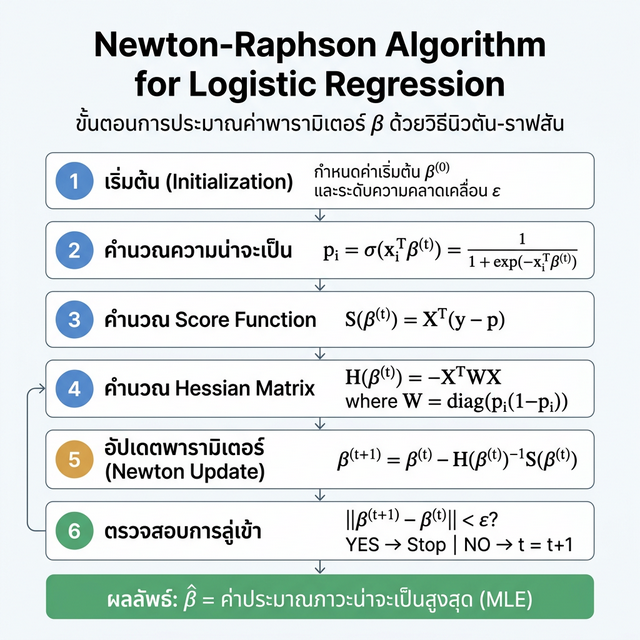
\includegraphics[width=0.8\textwidth]{CH3_NewtonRaphson_Workflow.png}
	\caption{ขั้นตอนการทำงานของอัลกอริทึมของนิวตันในการประมาณค่าพารามิเตอร์ $\beta$}
	\label{fig:newton_algo}
\end{figure}

\textbf{กรณีศึกษาและการประยุกต์ใช้ด้วย Python}

ในการทำงานเชิงประจักษ์นั้น นำเสนอกลไกของอัลกอริทึมผ่านตัวอย่างการคำนวณ 2 กรณีศึกษา ดังนี้

\textbf{กรณีศึกษาที่ 1: หลักการพื้นฐานการหาค่าราก (Root Finding)}

ในกรณีทั่วไป การหาค่า $x$ ที่ทำให้ $f(x) = 0$ สามารถทำได้โดยใช้อนุพันธ์ $f'(x)$ เป็นตัวนำทาง ดังสมการปรับปรุงค่า แสดงดังนี้

$$x_{t+1} = x_t - f(x_t)/f'(x_t)$$

\noindent
ภาพประกอบ \ref{fig:newton_root} แสดงการใช้ Python เพื่อหาค่ารากของสมการพหุนาม แสดงดังนี้

$$f(x) = x^3 - 2x - 2$$ 

\noindent
ซึ่งแสดงให้เห็นว่าเส้นสัมผัส (Tangent Line) ณ จุดปัจจุบันจะชี้ไปยังค่าประมาณที่ดีกว่าในรอบถัดไป

\begin{figure}[h!]
	\centering
	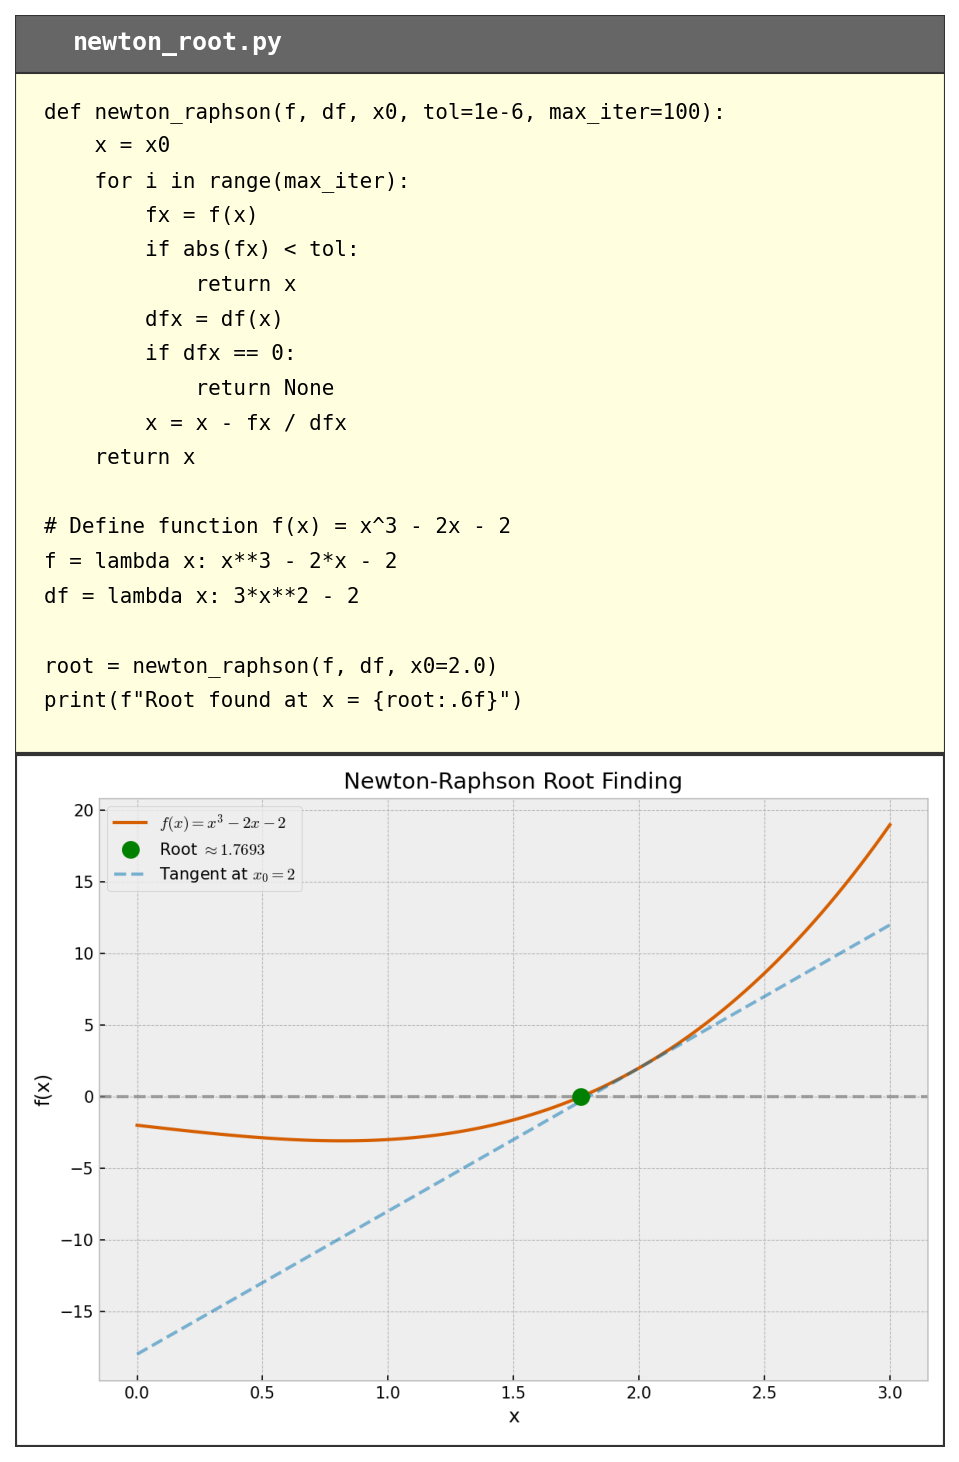
\includegraphics[width=0.8\textwidth]{CH3_newton_root.png}
	\caption{Python Code และผลลัพธ์การทำงานของวิธี Newton-Raphson แสดงเส้นสัมผัสและการลู่เข้าสู่ค่ารากของสมการ}
	\label{fig:newton_root}
\end{figure}

\textbf{กรณีศึกษาที่ 2: การหาค่าเหมาะสมที่สุด (Optimization) ในการถดถอยโลจิสติค}

สำหรับการประมาณค่าแบบภาวะน่าจะเป็นสูงสุด (MLE) เป้าหมายคือ การหา $\hat{\boldsymbol{\beta}}$ ที่ทำให้ฟังก์ชัน Log-Likelihood มีค่าสูงสุด การประยุกต์ใช้อัลกอริทึมของนิวตัน-ราฟสันในกรณีนี้จึงใช้สูตรการปรับปรุงค่าในรูปแบบเมทริกซ์ แสดงดังนี้ 

\begin{eqnarray} \nonumber
	\boldsymbol{\beta}^{(t+1)} &=& \boldsymbol{\beta}^{(t)} - \left[\mathbf{H}(\boldsymbol{\beta}^{(t)})\right]^{-1}\mathbf{S}(\boldsymbol{\beta}^{(t)}) \\
	&=& \boldsymbol{\beta}^{(t)} + [\mathbf{I}(\boldsymbol{\beta}^{(t)})]^{-1} \mathbf{S}(\boldsymbol{\beta}^{(t)})
\end{eqnarray}


โดยที่ $\mathbf{I}(\boldsymbol{\beta})$ คือเมทริกซ์ข้อมูลของฟิชเชอร์ (หรือลบของเมทริกซ์เฮสเซียน) ภาพประกอบ \ref{fig:newton_logistic} แสดงผลลัพธ์การใช้ Python เขียนอัลกอริทึมเพื่อปรับเส้นโค้ง Sigmoid ให้สอดคล้องกับข้อมูลสังเกตการณ์ ซึ่งเป็นหัวใจสำคัญของการเรียนรู้ในแบบจำลองแบบจำแนกประเภท (Classification)

\begin{figure}[h!]
	\centering
	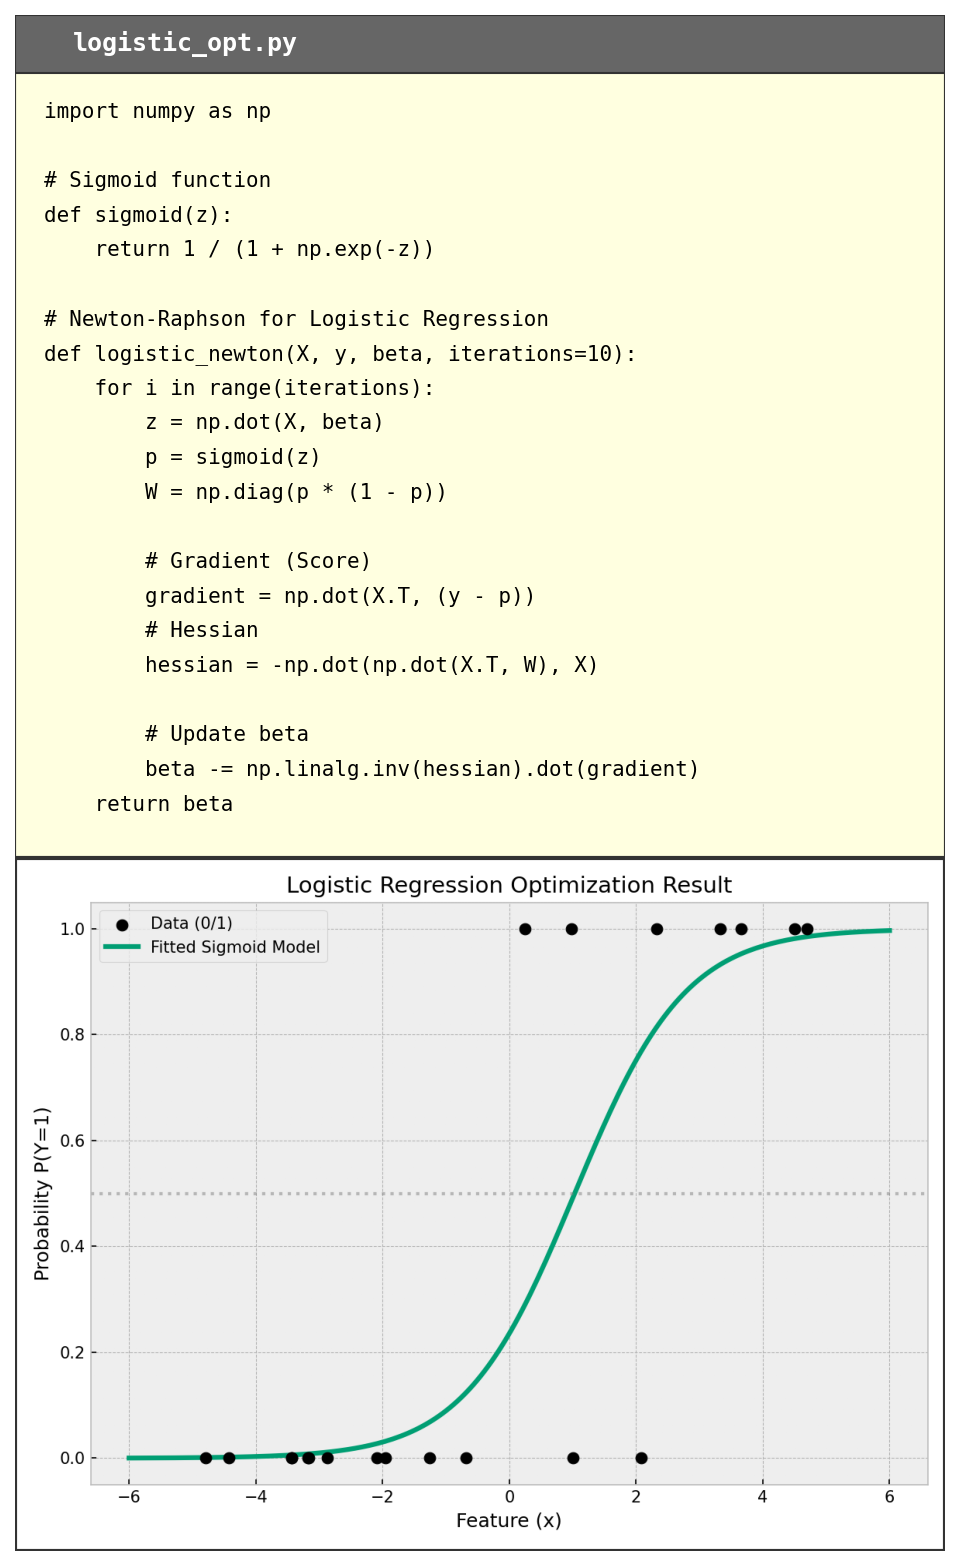
\includegraphics[width=0.8\textwidth]{CH3_newton_logistic.png}
	\caption{Python Code และผลลัพธ์การประมาณค่าพารามิเตอร์สำหรับการถดถอยโลจิสติค พร้อมกราฟแสดงความน่าจะเป็นที่ทำนายได้}
	\label{fig:newton_logistic}
\end{figure}

การนำเสนอในรูปแบบนี้ช่วยยืนยันว่า แม้สมการทางคณิตศาสตร์จะมีความซับซ้อน แต่สามารถแปลงเป็นขั้นตอนวิธีที่มีประสิทธิภาพทางคอมพิวเตอร์และให้ผลลัพธ์ที่แม่นยำได้

\subsubsection{อัลกอริทึม Adam}

อัลกอริทึม Adam (Adaptive Moment Estimation) ได้รับการนำเสนอโดย Kingma และ Ba ในปี 2015 เป็นวิธีการหาค่าเหมาะสมที่สุด (Optimization) ที่ผสมผสานข้อดีของ 2 แนวคิดสำคัญเข้าด้วยกัน ได้แก่ 

\begin{itemize}
	\item \textbf{Momentum (First Moment Estimate)} คือ การประมาณโมเมนต์อันดับที่หนึ่ง ซึ่งใช้ค่าเฉลี่ยเคลื่อนที่แบบเอ็กซ์โพเนนเชียล (Exponential Moving Average: EMA) ของเกรเดียนต์ แสดงดังนี้

	$$\mathbf{m}_t = \beta_1 \mathbf{m}_{t-1} + (1 - \beta_1)\mathbf{g}_t$$

	โดยที่ $\beta_1 \in [0, 1)$ แทนพารามิเตอร์แสดงอัตราการลดลงแบบเลขชี้กำลังสำหรับการประมาณค่าโมเมนต์แรก (ค่าเริ่มต้นที่แนะนำคือ $\beta_1 = 0.9$) และ $\mathbf{m}_t$ แทนการประมาณค่าคาดหวัง (Mean) ของเกรเดียนต์ ซึ่งทำหน้าที่สะสมทิศทางการปรับค่าจากรอบการคำนวณก่อนหน้า ช่วยรักษาทิศทางให้มีความต่อเนื่องและลดการแกว่ง (Oscillation) โดยกำหนดให้ $\mathbf{m}_0 = \mathbf{0}$



	\item \textbf{RMSProp (Second Moment Estimate)} คือโมเมนต์อันดับที่สองแบบไม่ปรับศูนย์กลาง (Uncentered Second Moment) ของเกรเดียนต์ ซึ่งใช้ค่าเฉลี่ยเคลื่อนที่แบบเอ็กซ์โพเนนเชียลของของเกรเดียนต์กำลังสอง แสดงดังนี้

	$$\mathbf{v}_t = \beta_2 \mathbf{v}_{t-1} + (1 - \beta_2)\mathbf{g}_t^2$$

	โดยที่ $\beta_2 \in [0, 1)$ แทนพารามิเตอร์อัตราการลดลงแบบเอ็กซ์โพเนนเชียลสำหรับการประมาณค่าโมเมนต์ที่สอง (ค่าเริ่มต้นที่แนะนำคือ $\beta_2 = 0.999$) และ $\mathbf{v}_0 = \mathbf{0}$

	\noindent
	ด้วยหลักการเดียวกันกับการคลี่สมการของ $\mathbf{m}_t$ จะได้

	$$\mathbf{v}_t = (1-\beta_2)\sum_{i=1}^{t}\beta_2^{t-i}\,\mathbf{g}_i^2$$

	\noindent
	ค่า $\mathbf{v}_t$ นี้เป็นการประมาณโมเมนต์อันดับที่สองแบบไม่ปรับศูนย์กลาง ของเกรเดียนต์ ซึ่งสะท้อนถึงขนาดของเกรเดียนต์แบบถ่วงน้ำหนักตามเวลา ทำให้สามารถปรับขนาดอัตราการเรียนรู้ (Learning Rate) ให้เหมาะสมกับแต่ละพารามิเตอร์อย่างอัตโนมัติ กล่าวคือ

	\begin{itemize}
		\item[] พารามิเตอร์ที่มีเกรเดียนต์ขนาดใหญ่สม่ำเสมอ ($\mathbf{v}_t$ มีค่ามาก) $\Rightarrow$ อัตราการเรียนรู้ \textbf{ลดลง}
		
		\item[] พารามิเตอร์ที่มีเกรเดียนต์ขนาดเล็ก ( $\mathbf{v}_t$ มีค่าน้อย) $\Rightarrow$ อัตราการเรียนรู้ \textbf{เพิ่มขึ้น}
	\end{itemize}

	ค่า $\beta_2 = 0.999$ ที่สูงกว่า $\beta_1 = 0.9$ ทำให้ $\mathbf{v}_t$ มีความเสถียรกว่า $\mathbf{m}_t$ กล่าวคือ $\mathbf{v}_t$ เฉลี่ยเกรเดียนต์กำลังสองในช่วงเวลาที่ยาวนานกว่ามาก  ซึ่งป้องกันการเปลี่ยนแปลงขนาดก้าวอย่างรวดเร็วเกินไป
\end{itemize}

จากข้างต้นค่าเฉลี่ยเคลื่อนที่แบบเอ็กซ์โพเนนเชียล (Exponential Moving Average: EMA) เป็นวิธีการถ่วงน้ำหนักข้อมูลในอดีตที่ให้ความสำคัญ (น้ำหนัก) กับข้อมูลล่าสุดมากกว่าข้อมูลในอดีต โดยน้ำหนักจะลดลงแบบเรขาคณิต (Geometric Decay) ซึ่งแตกต่างจากค่าเฉลี่ยเคลื่อนที่แบบธรรมดา (Simple Moving Average: SMA) ที่ให้น้ำหนักเท่ากันกับข้อมูลทุกจุด สำหรับความเข้าใจโครงสร้างของ EMA ใช้หลักการคลี่สมการวนซ้ำ จะได้ว่า 

\begin{eqnarray} \nonumber
	\mathbf{m}_t &=& \beta_1 \mathbf{m}_{t-1} + (1 - \beta_1)\mathbf{g}_t \\ \nonumber
	&=& \beta_1 [\beta_1 \mathbf{m}_{t-2} + (1-\beta_1)\mathbf{g}_{t-1}] + (1-\beta_1)\mathbf{g}_t \\ \nonumber
	&=& \beta_1^2 \mathbf{m}_{t-2} + (1-\beta_1)\beta_1\mathbf{g}_{t-1} + (1-\beta_1)\mathbf{g}_t \\ \nonumber
	&\vdots& \\ \nonumber
	&=& (1-\beta_1)\sum_{i=1}^{t}\beta_1^{t-i}\,\mathbf{g}_i + \beta_1^t\,\mathbf{m}_0
\end{eqnarray}

\noindent
เนื่องจาก $\mathbf{m}_0 = \mathbf{0}$ จึงได้

$$\mathbf{m}_t = (1-\beta_1)\sum_{i=1}^{t}\beta_1^{t-i}\,\mathbf{g}_i$$

\noindent
จากสมการข้างต้นจะเห็นว่าเกรเดียนต์ ณ รอบที่ $i$ จะได้รับน้ำหนัก (Weight) $w_i = (1-\beta_1)\,\beta_1^{t-i}$ ซึ่งมีคุณสมบัติสำคัญ ดังนี้

\begin{itemize}
	\item เกรเดียนต์ล่าสุด ($i = t$) มีน้ำหนัก $(1-\beta_1)$ มากที่สุด
	\item เกรเดียนต์เก่ากว่า 1 รอบ ($i = t-1$) มีน้ำหนัก $(1-\beta_1)\beta_1$
	\item เกรเดียนต์เก่ากว่า 2 รอบ ($i = t-2$) มีน้ำหนัก $(1-\beta_1)\beta_1^2$
	\item น้ำหนักทั้งหมดรวมกันตามอนุกรมเรขาคณิต: $\sum_{i=1}^{t} (1-\beta_1)\beta_1^{t-i} = 1 - \beta_1^t \approx 1$ เมื่อ $t$ มีค่ามาก
\end{itemize}


\noindent
สำหรับ $\mathbf{g}_t = \nabla_{\boldsymbol{\beta}} \mathcal{L}(\boldsymbol{\beta}^{(t)})$ คือเกรเดียนต์ของฟังก์ชันค่าสูญเสีย (Loss Function) ณ รอบการคำนวณที่ $t$ ในบริบทของการถดถอยโลจิสติค ฟังก์ชันค่าสูญเสียที่ใช้ทั่วไปคือ Negative Log-Likelihood ซึ่งสัมพันธ์กับฟังก์ชันลอการิทึมภาวะน่าจะเป็น $\ell(\boldsymbol{\beta})$ ที่ได้แสดงการพิสูจน์ไว้ในหัวข้อก่อนหน้า โดยกำหนดให้ $\mathcal{L}(\boldsymbol{\beta}) = -\ell(\boldsymbol{\beta})$ ดังนั้นเกรเดียนต์ของฟังก์ชันค่าสูญเสียจึงเท่ากับลบของฟังก์ชันคะแนน (Score Function) ที่ได้พิสูจน์ไว้แล้ว กล่าวคือ
$$\mathbf{g}_t = \nabla_{\boldsymbol{\beta}} \mathcal{L}(\boldsymbol{\beta}^{(t)}) = -\mathbf{S}(\boldsymbol{\beta}^{(t)}) = -\mathbf{X}^{T}(\mathbf{y} - \mathbf{p}^{(t)}) = \mathbf{X}^{T}(\mathbf{p}^{(t)} - \mathbf{y})$$
ความสัมพันธ์นี้แสดงให้เห็นว่าอัลกอริทึม Adam ใช้ข้อมูลจากอนุพันธ์อันดับที่หนึ่งของ Log-Likelihood เช่นเดียวกับอัลกอริทึมนิวตัน-ราฟสัน แต่ไม่จำเป็นต้องคำนวณอนุพันธ์อันดับที่สอง (เมทริกซ์เฮสเซียน) แต่อย่างใด



นอกจากนี้อัลกอริทึม Adam ยังใช้กลไกการแก้ไขความเอนเอียง (Bias Correction) ผ่าน $\hat{\mathbf{m}}_t = \mathbf{m}_t/(1-\beta_1^t)$ และ $\hat{\mathbf{v}}_t = \mathbf{v}_t/(1-\beta_2^t)$ เพื่อชดเชยการประมาณค่าที่ต่ำเกินไปในช่วงต้นของการฝึกสอน ทำให้สูตรการปรับปรุงค่าพารามิเตอร์มีรูปแบบดังนี้
$$\boldsymbol{\beta}^{(t+1)} = \boldsymbol{\beta}^{(t)} - \frac{\alpha}{\sqrt{\hat{\mathbf{v}}_t} + \epsilon}\hat{\mathbf{m}}_t$$

\noindent
โดยที่ 

$\alpha$ แทน อัตราการเรียนรู้ (ค่าเริ่มต้นที่แนะนำคือ $0.001$) ซึ่งเป็นสัดส่วนที่น้ำหนักจะถูกอัปเดตค่าที่มากขึ้น (เช่น 0.3) จะทำให้การเรียนรู้ในช่วงแรกเร็วขึ้นก่อนที่อัตราจะถูกอัปเดต ค่าที่น้อยลง (เช่น 1.0E-5) จะทำให้การเรียนรู้ช้าลงอย่างมากในระหว่างการฝึกสอน

$\epsilon$ แทน ค่าคงที่ขนาดเล็กเพื่อป้องกันการหารด้วยศูนย์ \\


สำหรับขั้นตอนการทำงานของอัลกอริทึม Adam แสดงดังภาพ \ref{fig:Adam_algo} เมื่อเปรียบเทียบกับอัลกอริทึมนิวตัน-ราฟสันที่กล่าวข้างต้น Adam มีข้อได้เปรียบในด้านความเหมาะสมสำหรับชุดข้อมูลขนาดใหญ่ (Large-scale Data) เนื่องจากใช้เพียงอนุพันธ์อันดับที่หนึ่ง (First-order Method) โดยไม่ต้องคำนวณหรือกลับเมทริกซ์เฮสเซียนซึ่งมีต้นทุนการคำนวณสูง ($O(k^3)$) อย่างไรก็ตาม นิวตัน-ราฟสันยังคงมีอัตราการลู่เข้าที่เร็วกว่า (Quadratic vs.\ Linear Convergence) สำหรับปัญหาขนาดเล็กถึงปานกลางที่มีโครงสร้างทางคณิตศาสตร์ที่ชัดเจน


\begin{figure}[h!]
	\centering
	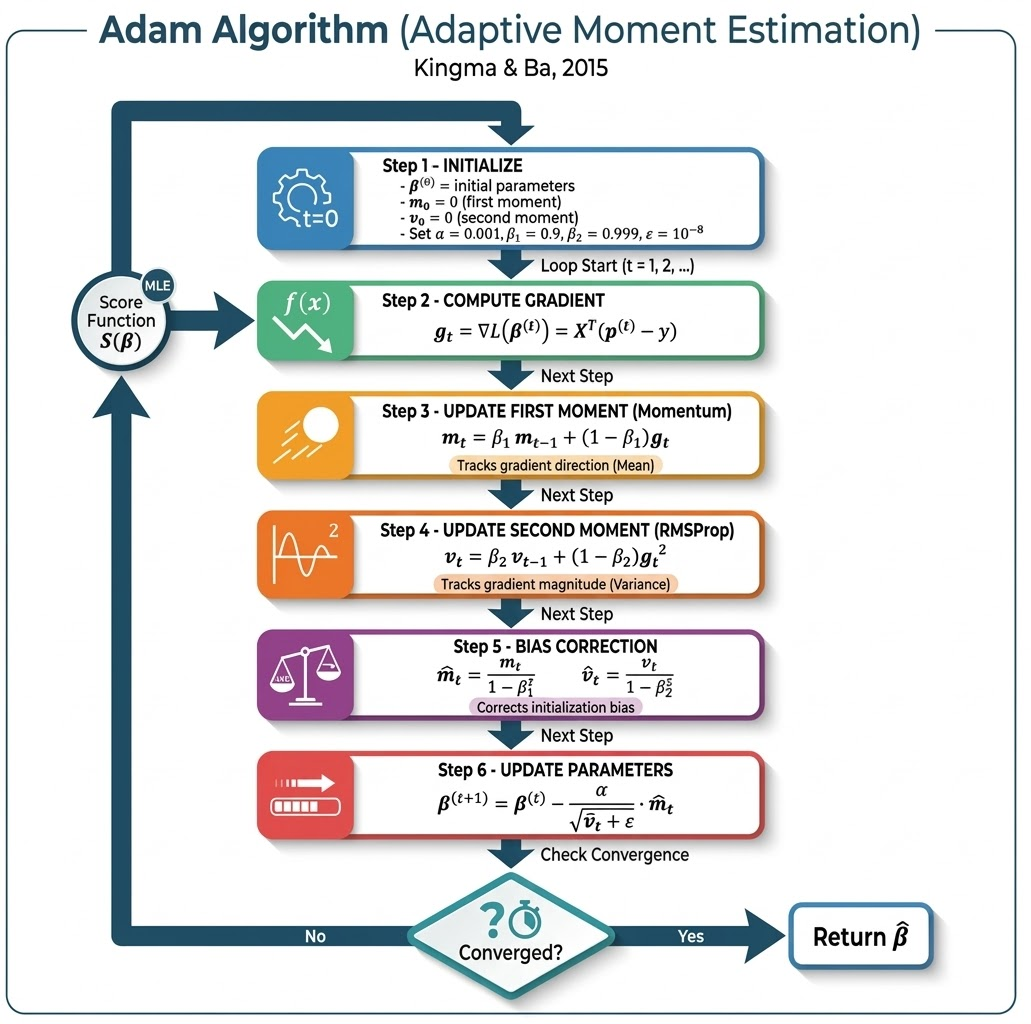
\includegraphics[width=0.9\textwidth]{CH3_AdamAlgorithm.png}
	\caption{ขั้นตอนการทำงานของอัลกอริทึม Adam ในการประมาณค่าารามิเตอร์ $\beta$}
	\label{fig:Adam_algo}
\end{figure}


\paragraph{การพิสูจน์ความเอนเอียงของค่าประมาณ $\mathbf{m}_t$ และที่มาของ Bias Correction}

เนื่องจากค่าเริ่มต้น $\mathbf{m}_0 = \mathbf{0}$ การคลี่สมการเวียนเกิด (Recurrence) ของ $\mathbf{m}_t$ จะได้

$$\mathbf{m}_t = (1 - \beta_1)\sum_{i=1}^{t} \beta_1^{t-i}\,\mathbf{g}_i$$

\noindent
เมื่อหาค่าคาดหวังทั้งสองข้าง ภายใต้สมมติฐานว่าเกรเดียนต์ที่แท้จริงมีค่าคงที่ $\mathbb{E}[\mathbf{g}_i] = \mathbf{g}$ สำหรับทุก $i$ จะได้ว่า

\begin{eqnarray} \nonumber
	\mathbb{E}[\mathbf{m}_t] &=& \mathbb{E}\left[(1-\beta_1)\sum_{i=1}^{t}\beta_1^{t-i}\,\mathbf{g}_i\right] \\ \nonumber
	&=& \mathbf{g}\cdot(1-\beta_1)\sum_{i=1}^{t}\beta_1^{t-i} \\ \nonumber
	&=& \mathbf{g}\cdot(1-\beta_1)\cdot\frac{1-\beta_1^t}{1-\beta_1} \\ \nonumber
	&=& \mathbf{g}\cdot(1-\beta_1^t)
\end{eqnarray}

\noindent
จะเห็นว่า $\mathbb{E}[\mathbf{m}_t] = \mathbf{g}(1 - \beta_1^t) \neq \mathbf{g}$ กล่าวคือ $\mathbf{m}_t$ เป็นตัวประมาณค่าแบบเอนเอียง (Biased Estimator) ของ $\mathbf{g}$ โดยเฉพาะอย่างยิ่งในรอบแรกๆ ที่ $\beta_1^t$ ยังมีค่าใกล้ 1 ค่า $\mathbf{m}_t$ จะมีขนาดเล็กกว่าความเป็นจริงอย่างมาก ดังนั้นจึงต้องทำการแก้ไขความเอนเอียงด้วยการหารด้วย $(1 - \beta_1^t)$ ดังนี้

$$\hat{\mathbf{m}}_t = \frac{\mathbf{m}_t}{1 - \beta_1^t} \quad \Longrightarrow \quad \mathbb{E}[\hat{\mathbf{m}}_t] = \mathbf{g}$$

\noindent
ด้วยหลักการเดียวกัน $\mathbf{v}_t$ ก็เป็นตัวประมาณค่าแบบเอนเอียงของ $\mathbb{E}[\mathbf{g}_t^2]$ จึงต้องใช้ Bias Correction เช่นเดียวกัน คือ $\hat{\mathbf{v}}_t = \mathbf{v}_t/(1 - \beta_2^t)$

\paragraph{ตัวอย่างเชิงตัวเลขการคำนวณอัลกอริทึม Adam}

เพื่อแสดงให้เห็นกลไกการทำงาน สมมติกรณี Logistic Regression ที่มีพารามิเตอร์เดี่ยว $\beta$ กำหนดค่าเริ่มต้น $\beta^{(0)} = 0$, $\alpha = 0.001$, $\beta_1 = 0.9$, $\beta_2 = 0.999$, $\epsilon = 10^{-8}$, $m_0 = 0$, $v_0 = 0$ และสมมติว่าเกรเดียนต์ $g_t$ ที่คำนวณได้ในแต่ละรอบมีค่าดังนี้

\begin{center}
\renewcommand{\arraystretch}{1.4}
\begin{tabular}{|c|c|c|c|c|c|c|c|}
\hline
$t$ & $g_t$ & $m_t$ & $v_t$ & $\hat{m}_t$ & $\hat{v}_t$ & $\Delta\beta$ & $\beta^{(t)}$ \\
\hline
0 & -- & 0 & 0 & -- & -- & -- & 0 \\
\hline
1 & 0.50 & 0.0500 & 0.000250 & 0.5000 & 0.2500  & $-0.001$ & $-0.001$ \\
\hline
2 & 0.45 & 0.0900 & 0.000452 & 0.4737 & 0.2262  & $-0.001$ & $-0.002$ \\
\hline
3 & 0.40 & 0.1210 & 0.000611 & 0.4431 & 0.2041  & $-0.001$ & $-0.003$ \\
\hline
\end{tabular}
\end{center}

\noindent
จากตารางจะเห็นว่า ในรอบแรก $m_1 = 0.9(0) + 0.1(0.50) = 0.05$ ก่อน Bias Correction มีค่าเพียง $0.05$ ซึ่งต่ำกว่าค่าเกรเดียนต์จริง $(0.50)$ มาก แต่หลังจากทำ Bias Correction $\hat{m}_1 = 0.05/(1-0.9^1) = 0.50$ กลับมาสะท้อนค่าที่แท้จริง นอกจากนี้ ค่า $\hat{v}_t$ ที่ลดลงทำให้ขนาดก้าวมีการปรับตัวอย่างอัตโนมัติ แสดงให้เห็นถึงคุณสมบัติ Adaptive Learning Rate ของอัลกอริทึม Adam

\begin{table}[h!]
\centering
\caption{การเปรียบเทียบอัลกอริทึมการหาค่าเหมาะสมที่สุดสำหรับการประมาณค่าพารามิเตอร์}
\label{tab:optimizer_compare}
\renewcommand{\arraystretch}{1.3}
\small
\begin{tabular}{|l|c|c|c|c|}
\hline
\textbf{คุณสมบัติ} & \textbf{SGD} & \textbf{AdaGrad} & \textbf{RMSProp} & \textbf{Adam} \\
\hline
อันดับของอนุพันธ์ & 1 & 1 & 1 & 1 \\
\hline
Adaptive LR & ไม่มี & มี & มี & มี \\
\hline
Momentum & ไม่มี & ไม่มี & ไม่มี & มี \\
\hline
Bias Correction & -- & -- & ไม่มี & มี \\
\hline
ปัญหา LR ลดจนหยุด & ไม่มี & มี & ไม่มี & ไม่มี \\
\hline
Hyperparameters & $\alpha$ & $\alpha$ & $\alpha, \beta_2$ & $\alpha, \beta_1, \beta_2$ \\
\hline
เหมาะกับข้อมูลขนาดใหญ่ & ปานกลาง & ต่ำ & สูง & สูงมาก \\
\hline
\end{tabular}
\end{table}

\noindent
จากตาราง \ref{tab:optimizer_compare} จะเห็นว่าอัลกอริทึม Adam ผสมผสานข้อดีของทั้ง Adaptive Learning Rate จาก AdaGrad/RMSProp และ Momentum เข้าด้วยกัน พร้อมทั้งมีกลไก Bias Correction ที่ช่วยให้การประมาณค่าในรอบแรกๆ มีความแม่นยำ จึงเป็นอัลกอริทึมที่ได้รับความนิยมอย่างกว้างขวางในงานวิจัยและการประยุกต์ใช้ด้านการเรียนรู้ของเครื่อง (Machine Learning) ในปัจจุบัน

\textbf{กรณีศึกษาและการประยุกต์ใช้ด้วย Python โดยใช้อัลกอริทึม Adam}

ในการทำงานเชิงประจักษ์นั้น นำเสนอกลไกของอัลกอริทึม Adam ผ่านตัวอย่างการคำนวณที่สอดคล้องกับกรณีศึกษาของนิวตัน-ราฟสัน ดังนี้

\textbf{กรณีศึกษาที่ 1: การหาค่าต่ำสุดของฟังก์ชัน (Function Minimization)}

ในการทำความเข้าใจกลไกพื้นฐาน อัลกอริทึม Adam สามารถระบุค่าที่ทำให้ฟังก์ชันมีค่าต่ำสุด (Optimization) โดยใช้เพียงข้อมูลเกรเดียนต์ สมมติพิจารณาการหาค่าต่ำสุดของฟังก์ชันพาราโบลา แสดงดังนี้

$$f(x) = (x-2)^2$$

ซึ่งมีค่าต่ำสุดที่ $x^* = 2$ โดยมีอนุพันธ์ (เกรเดียนต์) คือ

$$f'(x) = g_t = 2(x-2)$$

\noindent
\textbf{การกำหนดค่าเริ่มต้น (Hyperparameters)}

\begin{center}
\renewcommand{\arraystretch}{1.3}
\begin{tabular}{|c|l|c|}
\hline
\textbf{สัญลักษณ์} & \textbf{ความหมาย} & \textbf{ค่าที่ใช้} \\
\hline
$x^{(0)}$ & ค่าเริ่มต้น & $0$ \\
\hline
$\alpha$ & อัตราการเรียนรู้ (Learning Rate) & $0.1$ \\
\hline
$\beta_1$ & อัตราการลดลงของ First moment & $0.9$ \\
\hline
$\beta_2$ & อัตราการลดลงของ Second moment & $0.999$ \\
\hline
$\epsilon$ & ค่าคงที่ป้องกันการหารด้วยศูนย์ & $10^{-8}$ \\
\hline
$m_0$ & ค่าเริ่มต้น First Moment & $0$ \\
\hline
$v_0$ & ค่าเริ่มต้น Second Moment & $0$ \\
\hline
\end{tabular}
\end{center}

\noindent
\textbf{การคำนวณในแต่ละขั้นตอนในการหาค่าต่ำสุดของฟังก์ชัน} $f(x) = (x-2)^2$ แสดงดังนี้

\paragraph{รอบที่ $t = 1$}

\begin{enumerate}
    \item \textbf{คำนวณเกรเดียนต์ }
    $$g_1 = 2(x^{(0)} - 2) = 2(0 - 2) = -4$$

    \item \textbf{อัปเดต First Moment } 
    $$m_1 = 0.9 \times 0 + (1 - 0.9) \times (-4) = 0 + 0.1 \times (-4) = -0.4$$

    \item \textbf{อัปเดต Second Moment } 
    $$v_1 = 0.999 \times 0 + (1 - 0.999) \times (-4)^2 = 0 + 0.001 \times 16 = 0.016$$

    \item \textbf{Bias Correction } 
    $$\hat{m}_1 = \frac{-0.4}{1 - 0.9^1} = \frac{-0.4}{0.1} = -4.0$$
    $$\hat{v}_1 = \frac{0.016}{1 - 0.999^1} = \frac{0.016}{0.001} = 16.0$$

    \item \textbf{อัปเดต $x$ } 
    $$x^{(1)} = 0 - \frac{0.1}{\sqrt{16.0} + 10^{-8}} \times (-4.0) = 0 - \frac{0.1}{4.0} \times (-4.0) = 0 + 0.1 = 0.1$$
\end{enumerate}

\paragraph{รอบที่ $t = 2$}

\begin{enumerate}
    \item \textbf{คำนวณเกรเดียนต์ } 
    $$g_2 = 2(0.1 - 2) = 2 \times (-1.9) = -3.8$$

    \item \textbf{อัปเดต First Moment } 
    $$m_2 = 0.9 \times (-0.4) + 0.1 \times (-3.8) = -0.36 - 0.38 = -0.74$$

    \item \textbf{อัปเดต Second Moment } 
    $$v_2 = 0.999 \times 0.016 + 0.001 \times (-3.8)^2 = 0.015984 + 0.001 \times 14.44 = 0.015984 + 0.01444 = 0.030424$$

    \item \textbf{Bias Correction } 
    $$\hat{m}_2 = \frac{-0.74}{1 - 0.9^2} = \frac{-0.74}{1 - 0.81} = \frac{-0.74}{0.19} \approx -3.8947$$
    $$\hat{v}_2 = \frac{0.030424}{1 - 0.999^2} = \frac{0.030424}{1 - 0.998001} = \frac{0.030424}{0.001999} \approx 15.2196$$

    \item \textbf{อัปเดต $x$ } 
    $$x^{(2)} = 0.1 - \frac{0.1}{\sqrt{15.2196} + 10^{-8}} \times (-3.8947) \approx 0.1 - \frac{0.1}{3.9012} \times (-3.8947) \approx 0.1 + 0.0998 = 0.1998$$
\end{enumerate}

\paragraph{รอบที่ $t = 3$}

\begin{enumerate}
    \item \textbf{คำนวณเกรเดียนต์ } 
    $$g_3 = 2(0.1998 - 2) = 2 \times (-1.8002) = -3.6004$$

    \item \textbf{อัปเดต First Moment } 
    $$m_3 = 0.9 \times (-0.74) + 0.1 \times (-3.6004) = -0.666 - 0.36004 = -1.02604$$

    \item \textbf{อัปเดต Second Moment } 
    $$v_3 = 0.999 \times 0.030424 + 0.001 \times (-3.6004)^2 = 0.030394 + 0.001 \times 12.9629 = 0.030394 + 0.012963 = 0.043357$$

    \item \textbf{Bias Correction } 
    $$\hat{m}_3 = \frac{-1.02604}{1 - 0.9^3} = \frac{-1.02604}{1 - 0.729} = \frac{-1.02604}{0.271} \approx -3.7862$$
    $$\hat{v}_3 = \frac{0.043357}{1 - 0.999^3} = \frac{0.043357}{1 - 0.997003} = \frac{0.043357}{0.002997} \approx 14.4665$$

    \item \textbf{อัปเดต $x$ } 
    $$x^{(3)} = 0.1998 - \frac{0.1}{\sqrt{14.4665} + 10^{-8}} \times (-3.7862) \approx 0.1998 - \frac{0.1}{3.8035} \times (-3.7862) \approx 0.1998 + 0.0995 = 0.2993$$
\end{enumerate}

\noindent
\textbf{ตารางสรุปผลการคำนวณค่าต่ำสุดของฟังก์ชัน} $f(x) = (x-2)^2$ 

\begin{center}
\renewcommand{\arraystretch}{1.4}
\small
\begin{tabular}{|c|c|c|c|c|c|c|c|}
\hline
$t$ & $x^{(t-1)}$ & $g_t$ & $m_t$ & $v_t$ & $\hat{m}_t$ & $\hat{v}_t$ & $x^{(t)}$ \\
\hline
1 & 0.0000 & $-4.0000$ & $-0.4000$ & $0.016000$ & $-4.0000$ & $16.0000$ & $0.1000$ \\
\hline
2 & 0.1000 & $-3.8000$ & $-0.7400$ & $0.030424$ & $-3.8947$ & $15.2196$ & $0.1998$ \\
\hline
3 & 0.1998 & $-3.6004$ & $-1.0260$ & $0.043357$ & $-3.7862$ & $14.4665$ & $0.2993$ \\
\hline
$\vdots$ & $\vdots$ & $\vdots$ & $\vdots$ & $\vdots$ & $\vdots$ & $\vdots$ & $\vdots$ \\
\hline
$\infty$ & $\cdots$ & $0$ & $0$ & $0$ & $0$ & $0$ & $2.0000$ \\
\hline
\end{tabular}
\end{center}

\begin{myBox}[]{สรุปการทำงานของอัลกอริทึม Adam ในกรณี Function Minimization}{}
\begin{itemize}
    \item \textbf{Momentum ช่วยเร่งความเร็ว:} ค่า $\hat{m}_t \approx -4$ ในช่วงแรก สะท้อนว่าเกรเดียนต์มีทิศทางสม่ำเสมอ (ทิศทางเพิ่ม $x$ เสมอ) Momentum สะสมพลังงานทำให้ก้าวมีขนาดใหญ่และเร็ว
    \item \textbf{Adaptive Learning Rate ปรับอัตโนมัติ:} $\hat{v}_t$ สะท้อนขนาดของเกรเดียนต์ในอดีต เมื่อ $x$ เข้าใกล้ $x^* = 2$ เกรเดียนต์จะลดลง ทำให้ $\hat{v}_t$ ลดลง และขนาดก้าวถูกควบคุมอย่างละเอียด ป้องกันการกระโดดข้ามจุดต่ำสุด
    \item \textbf{Bias Correction มีความสำคัญในรอบแรก:} ในรอบที่ 1 ค่า $m_1 = -0.4$ (เอนเอียงต่ำ) แต่หลัง Bias Correction กลายเป็น $\hat{m}_1 = -4.0$ ซึ่งสะท้อนเกรเดียนต์ที่แท้จริง ทำให้การปรับค่าในรอบแรกมีขนาดที่เหมาะสม
    \item \textbf{อัตราการลู่เข้า:} อัลกอริทึม Adam มีอัตราการลู่เข้าเชิงเส้น (Linear Convergence) แต่ก้าวแต่ละรอบมีขนาดประมาณ $\alpha = 0.1$ อย่างสม่ำเสมอในช่วงที่ $\hat{v}_t \approx \hat{m}_t^2$
\end{itemize}
\end{myBox}

อัลกอริทึมจะปรับทิศทางและขนาดก้าวตามโมเมนตัมและขนาดเกรเดียนต์สะสม ดังแสดงในผลลัพธ์ภาพประกอบ~\ref{fig:adam_root}

\begin{figure}[h!]
	\centering
	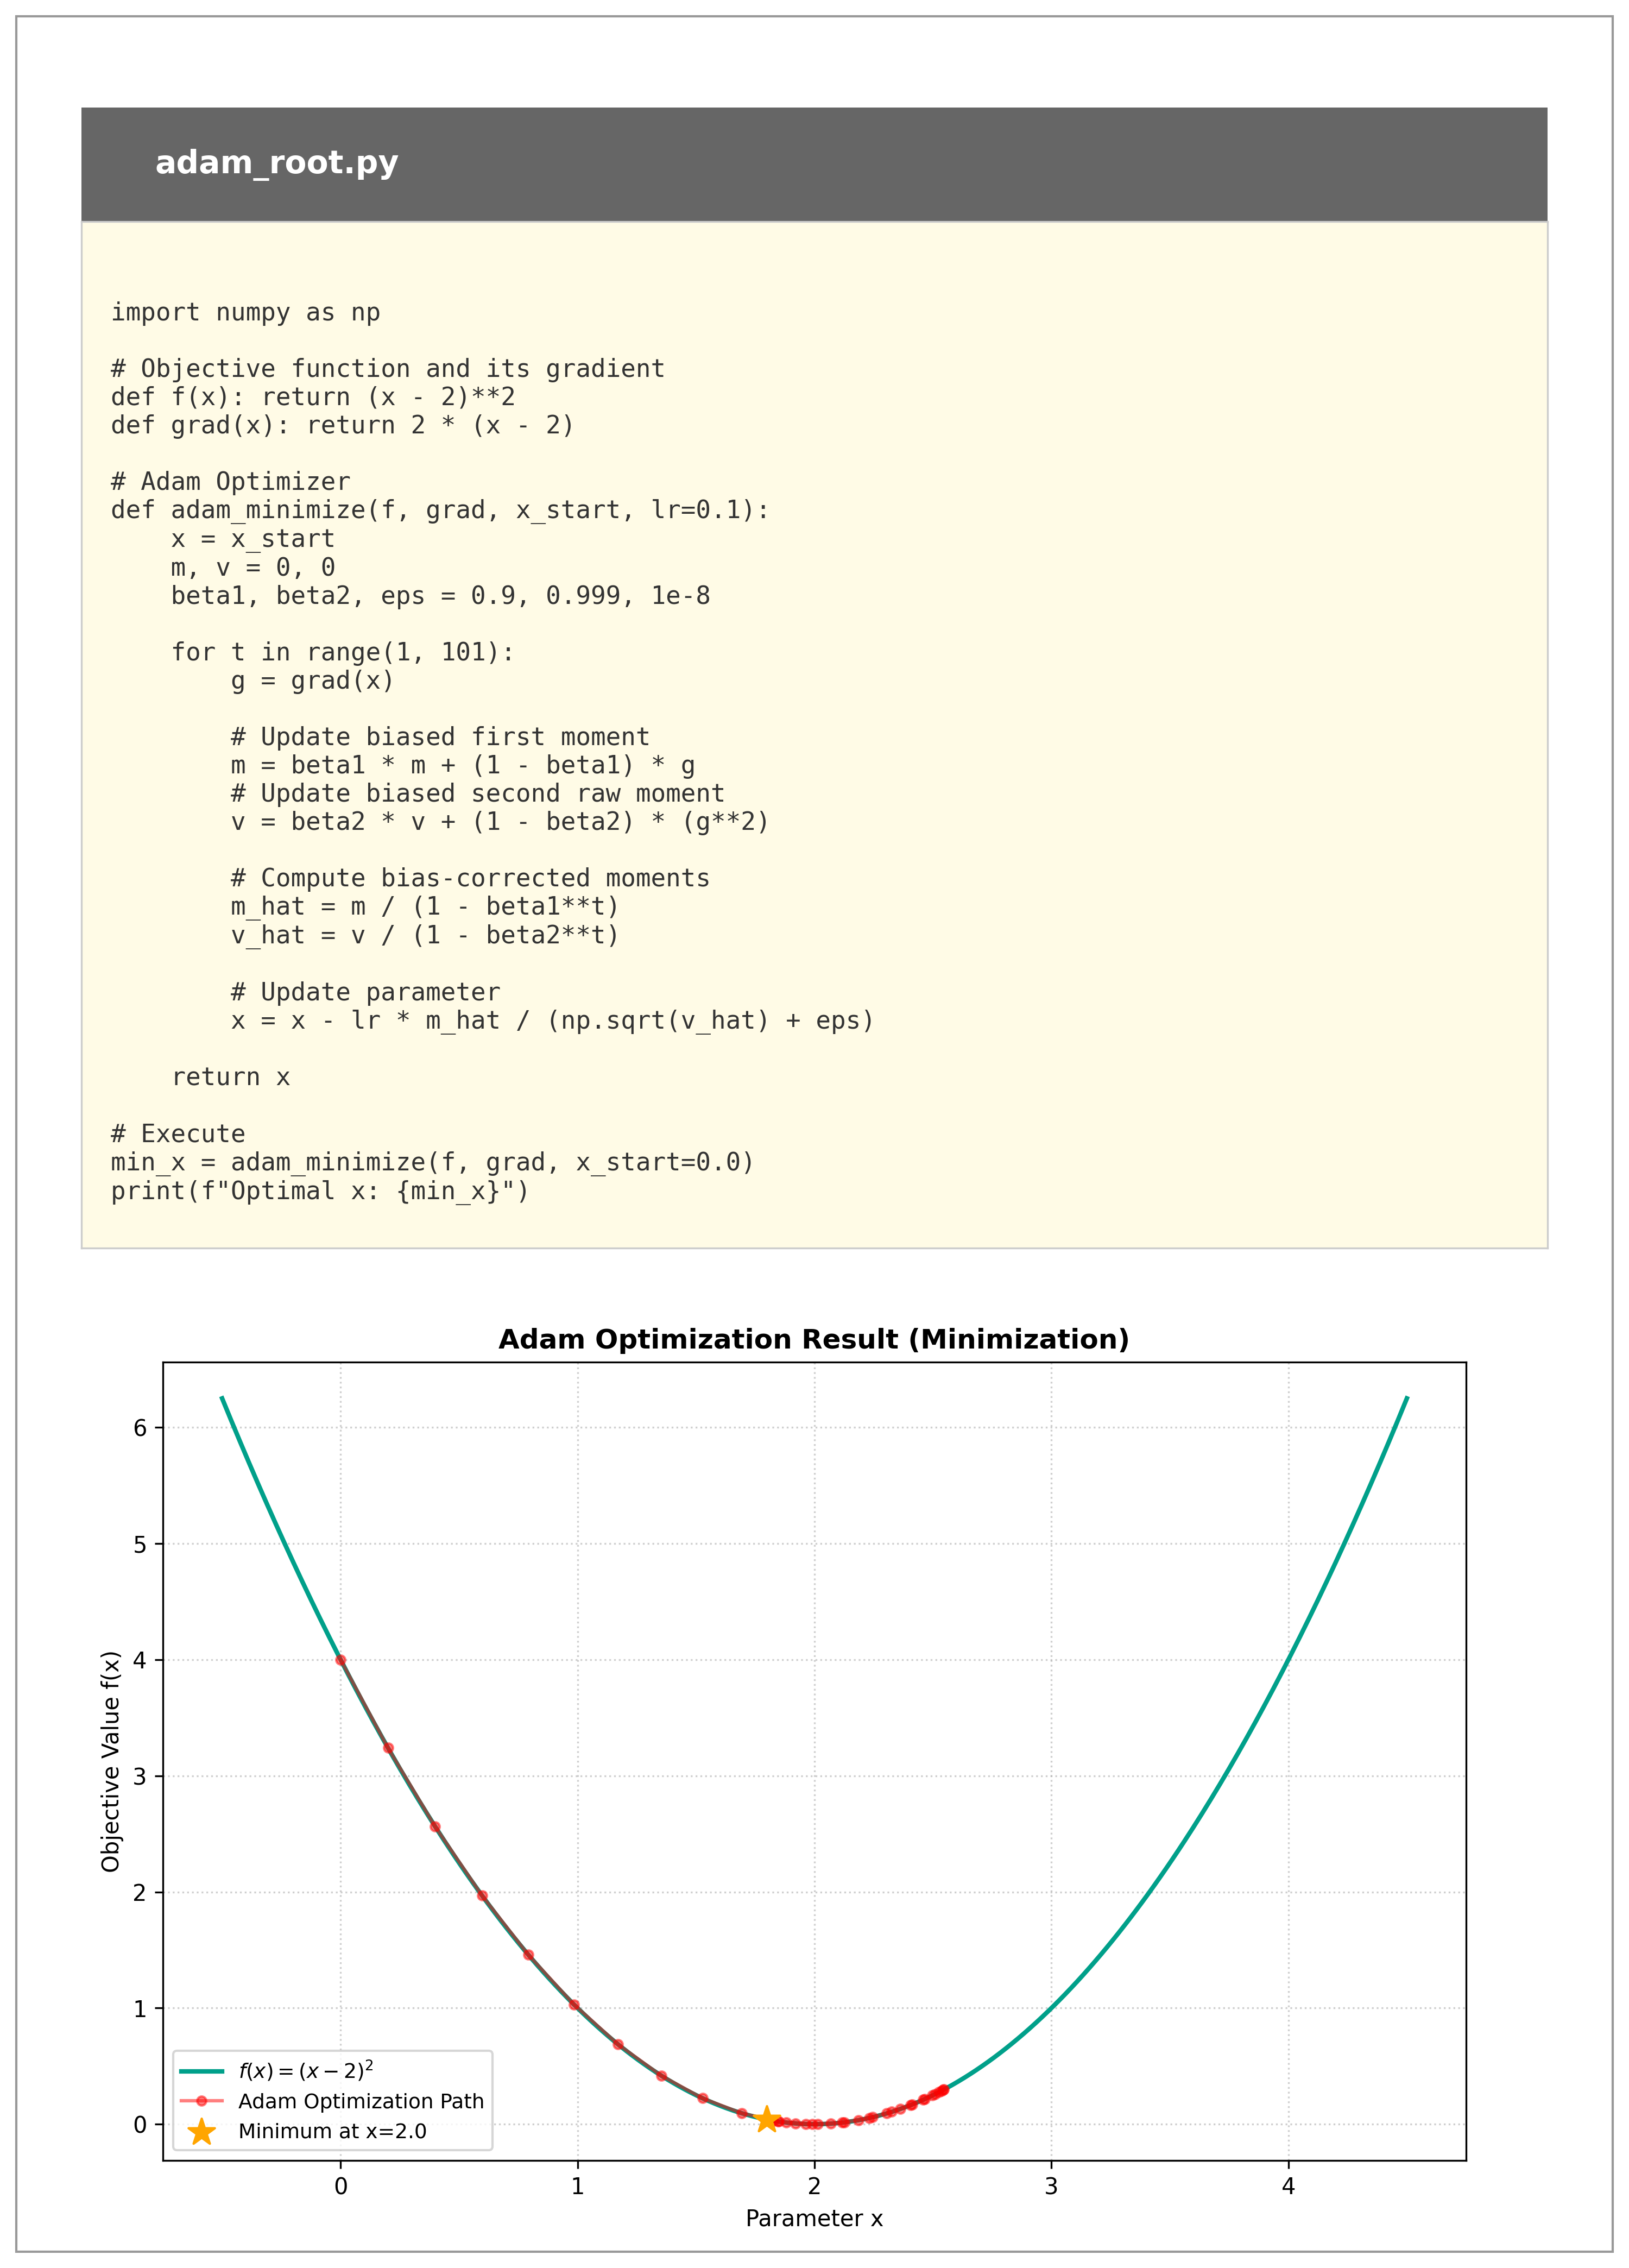
\includegraphics[width=1\textwidth]{CH3_adam_root.png}
	\caption{Python Code และผลลัพธ์การทำงานของวิธี Adam ในการหาค่าต่ำสุดของฟังก์ชันพาราโบลา โดยแสดงเส้นทางการลู่เข้าสู่จุดต่ำสุด}
	\label{fig:adam_root}
\end{figure}

\textbf{กรณีศึกษาที่ 2: การวิเคราะห์พฤติกรรมการซื้อสินค้า (Customer Purchase)}

สำหรับการวิเคราะห์พฤติกรรมการซื้อสินค้าพิจารณาจากตัวแปรเหล่านี้ ได้แก่ 
อายุ (Age) และเงินเดือน (Salary) เพื่อทำนายการตัดสินใจซื้อสินค้า (Buy: 1=ซื้อ, 0=ไม่ซื้อ) ข้อมูลแสดงดังตารางที่ \ref{tab:customer_data}

\begin{table}[h!]
\centering
\caption{ชุดข้อมูลตัวอย่างสำหรับใช้ทำนายการตัดสินใจซื้อสินค้า}
\label{tab:customer_data}
\small
\begin{tabular}{|c|c|c|c||c|c|c|c|}
\hline
$i$ & Age ($x_1$) & Salary ($x_2$) & Buy ($y$) & $i$ & Age ($x_1$) & Salary ($x_2$) & Buy ($y$) \\
\hline
1 & 20 & 20,000 & 0 & 6 & 45 & 90,000 & 1 \\
2 & 25 & 25,000 & 0 & 7 & 50 & 40,000 & 0 \\
3 & 30 & 30,000 & 0 & 8 & 55 & 95,000 & 1 \\
4 & 35 & 80,000 & 1 & 9 & 22 & 22,000 & 0 \\
5 & 40 & 35,000 & 0 & 10 & 48 & 85,000 & 1 \\
\hline
\end{tabular}
\end{table}

\noindent
\textbf{การประมาณค่าพารามิเตอร์ $\boldsymbol{\beta}$ ด้วยอัลกอริทึม Adam} แสดงดังนี้

สำหรับการคำนวณในเวคเตอร์ $\boldsymbol{\beta} = [\beta_0, \beta_1, \beta_2]^T$ โดยกำหนดค่าเริ่มแรก $\boldsymbol{\beta}^{(0)} = [0, 0, 0]^T$ และใช้อัตราการเรียนรู้ $\alpha = 0.01$ 

\paragraph{รอบที่ $t = 1$}
\begin{enumerate}
    \item \textbf{คำนวณความน่าจะเป็น ($p_i$)} 
    
    จากสมการโครงสร้าง $\hat{y}_i = \hat{\beta}_0 + \hat{\beta}_1 x_{i1} + \hat{\beta}_2 x_{i2}$ โดยค่าน้ำหนักเริ่มต้นคือ $\hat{\beta}_0 = \hat{\beta}_1 = \hat{\beta}_2 = 0$ แสดงการพิจารณาทีละชุดข้อมูลดังนี้
    
    ชุดข้อมูลที่ $i=1$ ($x_{11} = 20, x_{12} = 20,000, y_1 = 0$):
    \begin{eqnarray} \nonumber
        \hat{y}_1 &=& (0) + (0)(20) + (0)(20,000) = 0 \\ \nonumber
        p_1 &=& \frac{1}{1 + e^{-\hat{y}_1}} = \frac{1}{1 + e^{-0}} = 0.5
    \end{eqnarray}
    
    ชุดข้อมูลที่ $i=2$ ($x_{21} = 25, x_{22} = 25,000, y_2 = 0$):
    \begin{eqnarray} \nonumber
        \hat{y}_2 &=& (0) + (0)(25) + (0)(25,000) = 0 \\ \nonumber
        p_2 &=& \frac{1}{1 + e^{-\hat{y}_2}} = \frac{1}{1 + e^{-0}} = 0.5
    \end{eqnarray}
    
    \item \textbf{คำนวณเกรเดียนต์ ($\mathbf{g}_1$)} 
    
   รายละเอียดความสัมพันธ์ของสมการเวกเตอร์ $\mathbf{g} = \mathbf{X}^T(\mathbf{p} - \mathbf{y})$ เมื่อพิจารณา 2 ตัวอย่างแรก ($i=1, 2$) ในรูปแบบเมทริกซ์และเวกเตอร์ แสดงผลคูณได้ดังนี้:
    
    $$ \begin{bmatrix} g_{\beta_0} \\ g_{\beta_1} \\ g_{\beta_2} \end{bmatrix} = \underbrace{\begin{bmatrix} 1 & 1 \\ x_{11} & x_{21} \\ x_{12} & x_{22} \end{bmatrix}}_{\mathbf{X}^T} \underbrace{\begin{bmatrix} p_1 - y_1 \\ p_2 - y_2 \end{bmatrix}}_{(\mathbf{p} - \mathbf{y})} = \begin{bmatrix} 1(p_1 - y_1) + 1(p_2 - y_2) \\ x_{11}(p_1 - y_1) + x_{21}(p_2 - y_2) \\ x_{12}(p_1 - y_1) + x_{22}(p_2 - y_2) \end{bmatrix} $$
    
    แทนค่าตัวเลขจากตารางข้อมูลและผลการคำนวณในขั้นตอนก่อนหน้า:
    
   \begin{eqnarray} \nonumber
   g_{\beta_0} &=& (0.5-0) + (0.5-0) = 1.0  \\  \nonumber
   g_{\beta_1} &=& (0.5-0)(20) + (0.5-0)(25) = 10 + 12.5 = 22.5 \\ \nonumber
   g_{\beta_2} &=& (0.5-0)(20000) + (0.5-0)(25000) = 10000 + 12500 = 22500
   \end{eqnarray}
   
 
    
    
    \item \textbf{อัปเดตโมเมนต์และ Bias Correction} (แสดงเฉพาะ $\beta_1$)
    
    \begin{eqnarray} \nonumber
    	m_{1, \beta_1} &=& 0.9(0) + 0.1(22.5) = 2.25 \\ \nonumber
    	v_{1, \beta_1} &=& 0.999(0) + 0.001(22.5)^2 = 0.50625
    \end{eqnarray}

    จากข้างต้นจะได้ว่า $ \hat{m}_1 = 22.5$ และ $ \hat{v}_1 = 506.25$
    \item \textbf{อัปเดตพารามิเตอร์} 
    
    $$\beta_1^{(1)} = 0 - \frac{0.01}{\sqrt{506.25} + \epsilon}(22.5) = -0.01$$
\end{enumerate}

\noindent
\textbf{การทำนายผลลัพธ์ (Prediction)}
หลังจากการฝึกสอนจนครบถ้วน สมมติได้สมการ Logit ดังรูปที่แนบมา:
$$\hat{y} \approx -0.0224 - 0.3942(\text{Age}) + 0.0003(\text{Salary})$$

\noindent
\textbf{โจทย์ปัญหา:} จงทำนายโอกาสการซื้อของลูกค้าอายุ \textbf{42 ปี} และมีเงินเดือน \textbf{75,000 บาท}

\begin{enumerate}
	\item \textbf{การแทนค่า } แสดงดังนี้ 
	\begin{align*}
		\hat{y} &= -0.0224 - 0.3942(42) + 0.0003(75000) \\
		&= -0.0224 - 16.5564 + 22.5000 \\
		&= 5.9212
	\end{align*}
	
	\item \textbf{การคำนวณความน่าจะเป็น } แสดงดังนี้
	$$P(Y=1 | \text{Age}=42, \text{Salary}=75000) = p = \frac{1}{1 + e^{-5.9212}} \approx 0.9973$$
\end{enumerate}

ดังนั้น โอกาสที่ลูกค้าท่านนี้จะตัดสินใจซื้อสินค้าสูงถึงประมาณ \textbf{99.73\%}

\begin{myBox}[]{สรุปการประยุกต์ใช้ Adam}{}
การใช้อัลกอริทึม Adam ช่วยให้แบบจำลองสามารถจัดการกับตัวแปรที่มีสเกลต่างกันมาก (เช่น Age และ Salary) ได้อย่างมีประสิทธิภาพผ่านการปรับ Adaptive Learning Rate ทำให้ค่า $\beta$ ลู่เข้าสู่จุดที่เหมาะสมที่สุดเพื่อใช้ในการจำแนกกลุ่มลูกค้าได้อย่างแม่นยำ
\end{myBox}

\begin{figure}[h!]
	\centering
	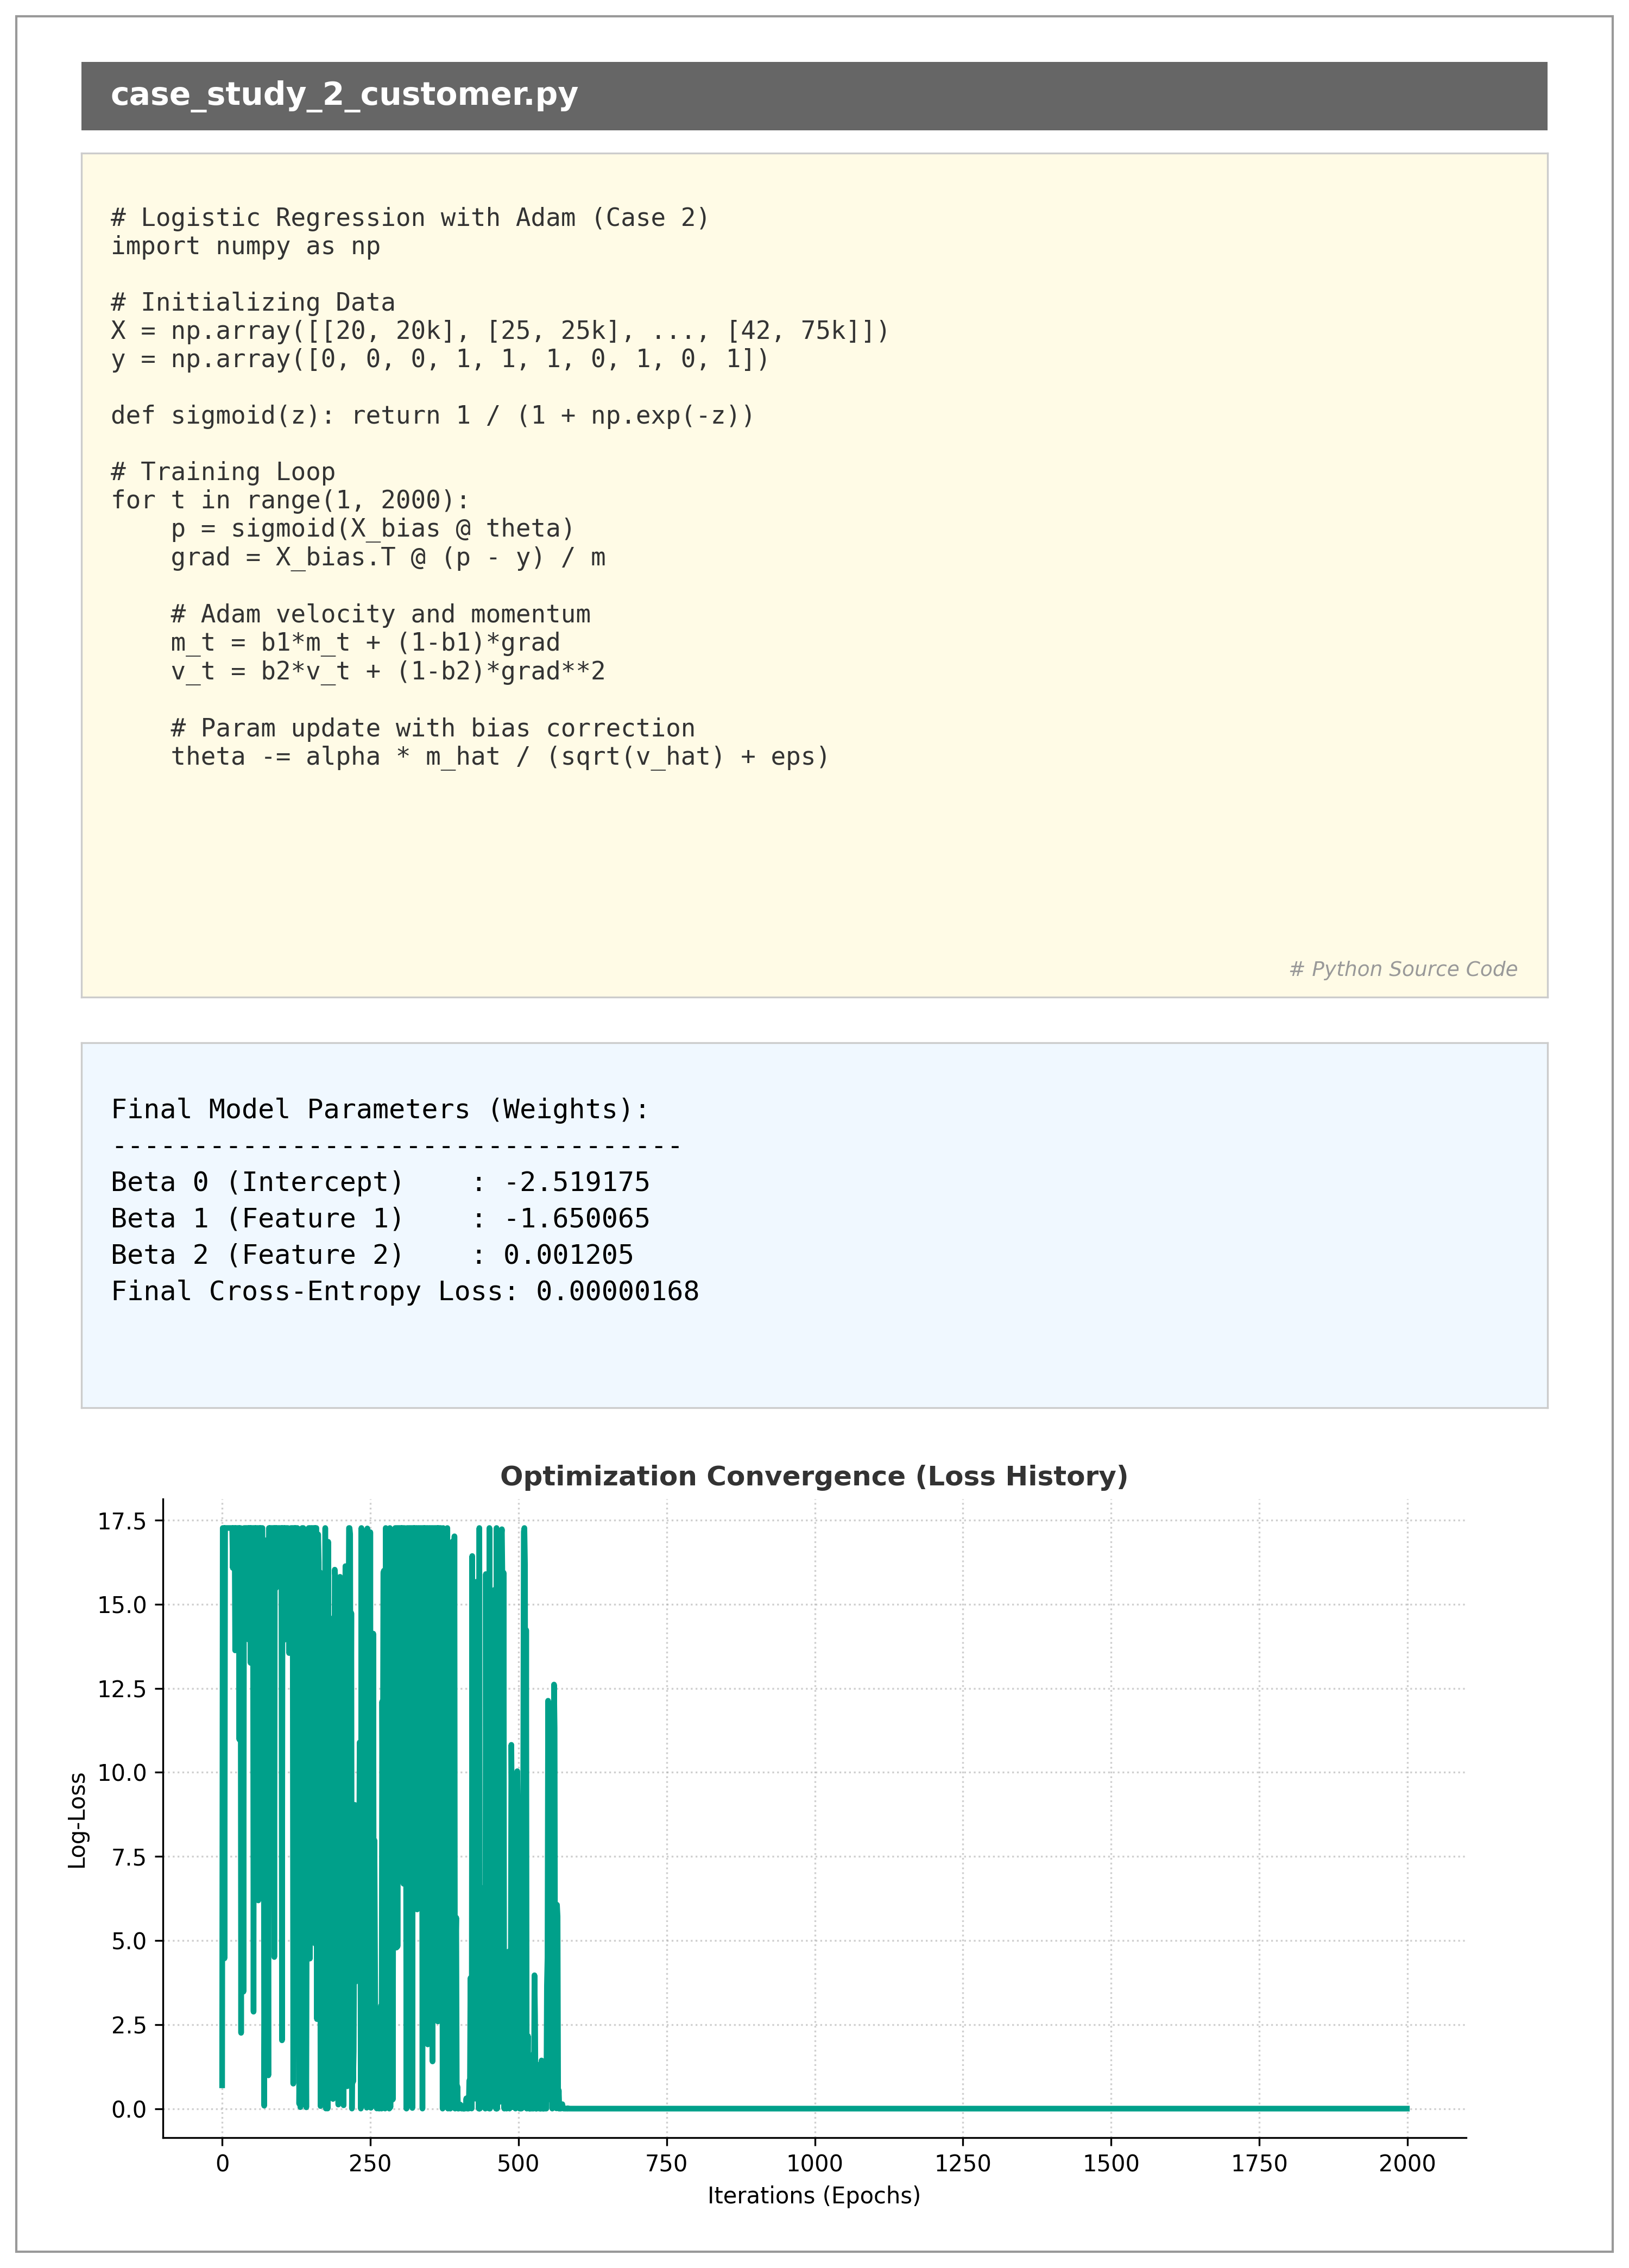
\includegraphics[width=1\textwidth]{CH3_case2_adam_results.png}
	\caption{Python Code และผลลัพธ์การประมาณค่าพารามิเตอร์ของกรณีศึกษาที่ 2 ด้วยอัลกอริทึม Adam พร้อมกราฟแสดงการลู่เข้าของค่าความสูญเสีย (Loss Curve)}
	\label{fig:case2_results}
\end{figure}

\textbf{กรณีศึกษาที่ 3: การประเมินความเสี่ยงต่อการเกิดโรคหัวใจ (Heart Disease Risk Assessment)}

ในวิทยาการระบาดและการแพทย์ การประเมินความเสี่ยงต่อการเกิดโรค (Risk Assessment) มักต้องพิจารณาปัจจัยร่วมหลายประการ พิจารณาชุดข้อมูลตัวอย่างของผู้ป่วย 10 ราย โดยมีตัวแปรทำนาย คือ อายุ (Age) และระดับคอเลสเตอรอล (Cholesterol) เพื่อทำนายสถานะการเกิดโรคหัวใจ (Disease Status) ดังตารางที่ \ref{tab:heart_disease_data}

\begin{table}[h!]
\centering
\caption{ชุดข้อมูลตัวอย่างของผู้ป่วยสำหรับใช้ในการประเมินความเสี่ยงการเกิดโรคหัวใจ}
\label{tab:heart_disease_data}
\begin{tabular}{|c|c|c|c|}
\hline
Subject & Age ($x_1$) & Cholesterol ($x_2$) & Disease Status ($y$) \\
\hline
1 & 25 & 180 & 0 \\
2 & 30 & 190 & 0 \\
3 & 45 & 220 & 1 \\
4 & 50 & 240 & 1 \\
5 & 60 & 260 & 1 \\
6 & 35 & 200 & 0 \\
7 & 40 & 210 & 0 \\
8 & 55 & 250 & 1 \\
9 & 65 & 280 & 1 \\
10 & 58 & 230 & 1 \\
\hline
\end{tabular}
\end{table}

\textbf{การประมาณค่าพารามิเตอร์ด้วยอับกอริทึม Adam}

กำหนดค่าพารามิเตอร์เริ่มต้น $\hat{\boldsymbol{\beta}}^{(0)} = [0, 0, 0]^T$ และอัตราการเรียนรู้ $\alpha = 0.01$

\paragraph{รอบที่ $t = 1$}
\begin{enumerate}
    \item \textbf{คำนวณความน่าจะเป็น ($p_i$)} 
    
    พิจารณา 2 ชุดข้อมูลแรก:
    
    ชุดข้อมูลที่ $i=1$ ($x_{11} = 25, x_{12} = 180, y_1 = 0$):
    \begin{eqnarray} \nonumber
        \hat{y}_1 &=& (0) + (0)(25) + (0)(180) = 0 \\ \nonumber
        p_1 &=& \frac{1}{1 + e^{-0}} = 0.5
    \end{eqnarray}
    
    ชุดข้อมูลที่ $i=2$ ($x_{21} = 30, x_{22} = 190, y_2 = 0$):
    \begin{eqnarray} \nonumber
        \hat{y}_2 &=& (0) + (0)(30) + (0)(190) = 0 \\ \nonumber
        p_2 &=& \frac{1}{1 + e^{-0}} = 0.5
    \end{eqnarray}
    
    \item \textbf{คำนวณเกรเดียนต์ ($\mathbf{g}_1$)} 
    
    ความสัมพันธ์ในรูปแบบเมทริกซ์ $\mathbf{g} = \mathbf{X}^T(\mathbf{p} - \mathbf{y})$ สำหรับ 2 ตัวอย่างแรก:
    
    $$ \begin{bmatrix} g_{\beta_0} \\ g_{\beta_1} \\ g_{\beta_2} \end{bmatrix} = \begin{bmatrix} 1 & 1 \\ 25 & 30 \\ 180 & 190 \end{bmatrix} \begin{bmatrix} 0.5 - 0 \\ 0.5 - 0 \end{bmatrix} = \begin{bmatrix} 0.5 + 0.5 \\ 12.5 + 15.0 \\ 90.0 + 95.0 \end{bmatrix} = \begin{bmatrix} 1.0 \\ 27.5 \\ 185.0 \end{bmatrix} $$
    
    \item \textbf{อัปเดตโมเมนต์และ Bias Correction} (แสดงตัวอย่างสำหรับ $\beta_1$)
    \begin{itemize}
        \item $m_1 = (0.9)(0) + (0.1)(27.5) = 2.75$
        \item $v_1 = (0.999)(0) + (0.001)(27.5)^2 = 0.75625$
        \item $\hat{m}_1 = 2.75 / (1 - 0.9^1) = 27.5$
        \item $\hat{v}_1 = 0.75625 / (1 - 0.999^1) = 756.25$
    \end{itemize}
    
    \item \textbf{อัปเดตพารามิเตอร์}
    $$\beta_1^{(1)} = 0 - \frac{0.01}{\sqrt{756.25} + \epsilon}(27.5) = -0.01$$
\end{enumerate}

\noindent
\textbf{การทำนายผลลัพธ์ (Prediction)}

หลังจากการวิเคราะห์ด้วยการถดถอยโลจิสติคพหุคูณ ได้สมการของ Log-odds (Logit) ดังนี้:
$$\ln \left( \frac{p}{1-p} \right) \approx -0.1394 + 6.9918(\text{Age}) - 1.3814(\text{Chol})$$

\noindent
\textbf{โจทย์ปัญหา:} จงประเมินความเสี่ยงในการเป็นโรคหัวใจสำหรับผู้ป่วยที่มีอายุ \textbf{52 ปี} และมีระดับคอเลสเตอรอล \textbf{235 mg/dL}

\begin{enumerate}
    \item \textbf{ขั้นตอนที่ 1 การคำนวณค่าลอจิต:} แทนค่าลงในสมการทำนายดังนี้
    \begin{align*}
        \hat{y} &= -0.1394 + 6.9918(52) - 1.3814(235) \\
        &= -0.1394 + 363.5736 - 324.6290 \\
        &= 38.8052
    \end{align*}
    
    \item \textbf{ขั้นตอนที่ 2 การคำนวณความน่าจะเป็น:}
    $$P(Y=1 | x_1=52, x_2=235) = p = \frac{1}{1 + e^{-38.8052}} \approx 1.0$$
\end{enumerate}

\noindent
\textbf{สรุป:} ผู้ป่วยรายนี้มีความเสี่ยงสูงมากในการเกิดโรคหัวใจ (ความน่าจะเป็นเกือบ 100\%) ซึ่งสอดคล้องกับแนวคิดทางการแพทย์ที่ว่าอายุที่มากขึ้นและระดับคอเลสเตอรอลที่สูงมักสัมพันธ์กับความเสี่ยงที่เพิ่มขึ้น (อย่างไรก็ตามค่าสัมประสิทธิ์ในสมการนี้เป็นค่าประมาณเพื่อการสาธิตเท่านั้น)

\begin{figure}[h!]
	\centering
	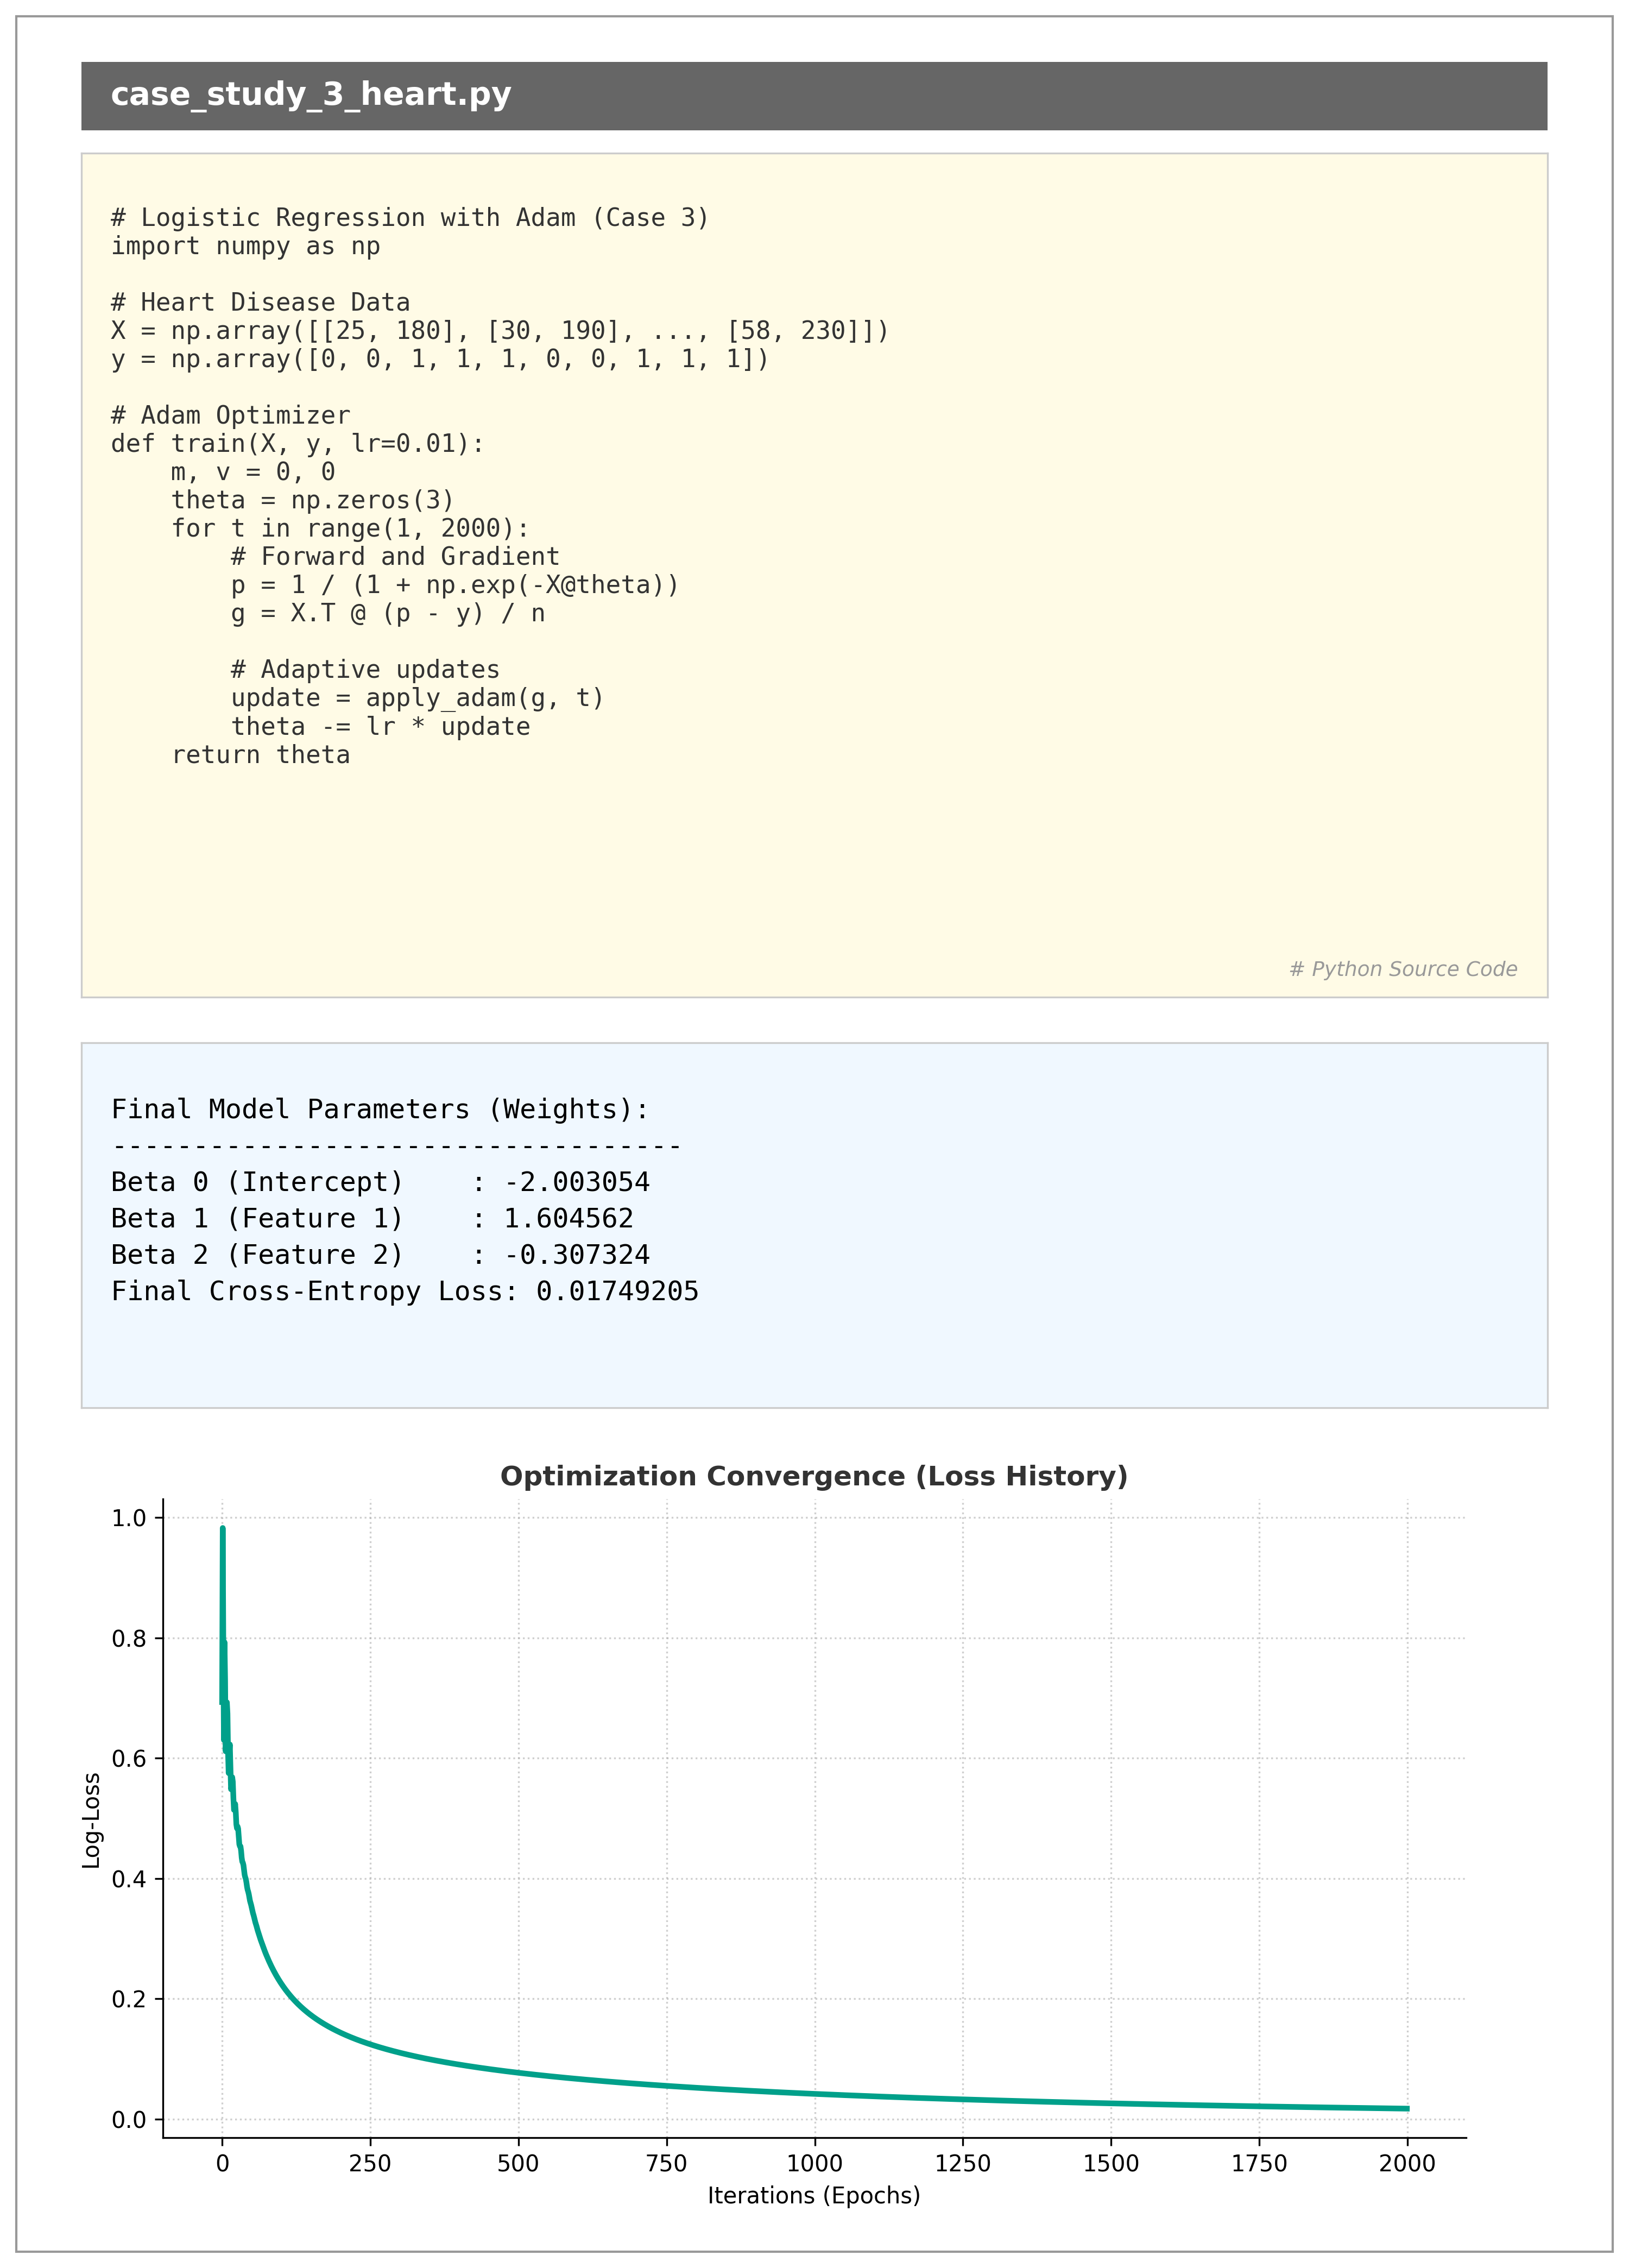
\includegraphics[width=1\textwidth]{CH3_case3_adam_results.png}
	\caption{Python Code และผลลัพธ์การประมาณค่าพารามิเตอร์ของกรณีศึกษาที่ 3 ด้วยอัลกอริทึม Adam พร้อมกราฟแสดงการลู่เข้าของค่าความสูญเสีย (Loss Curve)}
	\label{fig:case3_results}
\end{figure}



\textbf{กรณีศึกษาที่ 4: การประเมินความเสี่ยงสินเชื่อ (Credit Scoring)}

ในด้านการเงินและการธนาคาร การประเมินความเสี่ยงสินเชื่อ (Credit Scoring) เป็นปัญหาการจำแนกประเภทที่มีความสำคัญอย่างยิ่ง โดยมีวัตถุประสงค์เพื่อทำนายว่าผู้กู้จะผิดนัดชำระหนี้ (Default = 1) หรือไม่ (Default = 0) พิจารณาชุดข้อมูลตัวอย่างของผู้กู้ 10 ราย โดยมีตัวแปรทำนาย 5 ตัว ได้แก่ คะแนนเครดิต (Score), รายได้ต่อปี (Income k\$), สัดส่วนหนี้ต่อรายได้ (DTI \%), ประสบการณ์การทำงาน (Emp Yrs), และ วงเงินกู้ (Loan k\$) ดังตารางที่ \ref{tab:credit_data}

\begin{table}[h!]
\centering
\caption{ชุดข้อมูลตัวอย่างสำหรับการประเมินความเสี่ยงสินเชื่อ}
\label{tab:credit_data}
\renewcommand{\arraystretch}{1.2}
\small
\begin{tabular}{|c|c|c|c|c|c|c|}
\hline
\textbf{Subject} & \textbf{Score ($x_1$)} & \textbf{Income ($x_2$)} & \textbf{DTI ($x_3$)} & \textbf{Emp ($x_4$)} & \textbf{Loan ($x_5$)} & \textbf{Default ($y$)} \\
\hline
1 & 720 & 55 & 15 & 8  & 20 & 0 \\
2 & 680 & 40 & 22 & 5  & 25 & 0 \\
3 & 600 & 30 & 35 & 2  & 30 & 1 \\
4 & 750 & 80 & 10 & 15 & 40 & 0 \\
5 & 620 & 35 & 40 & 1  & 35 & 1 \\
6 & 700 & 60 & 18 & 10 & 28 & 0 \\
7 & 580 & 25 & 45 & 1  & 40 & 1 \\
8 & 660 & 45 & 25 & 6  & 22 & 0 \\
9 & 740 & 70 & 12 & 12 & 18 & 0 \\
10 & 610 & 28 & 38 & 2  & 32 & 1 \\
\hline
\end{tabular}
\end{table}

\textbf{การประมาณค่าพารามิเตอร์ด้วยอัลกอริทึม Adam}

กำหนดค่าพารามิเตอร์เริ่มต้น $\hat{\boldsymbol{\beta}}^{(0)} = [0, 0, 0, 0, 0, 0]^T$ และอัตราการเรียนรู้ $\alpha = 0.001$, $\beta_1 = 0.9$, $\beta_2 = 0.999$, $\epsilon = 10^{-8}$

\paragraph{รอบที่ $t = 1$}
\begin{enumerate}
    \item \textbf{คำนวณความน่าจะเป็น ($p_i$)}
    
    พิจารณา 2 ชุดข้อมูลแรก (ณ $t=0$, $\boldsymbol{\beta}^{(0)} = \mathbf{0}$):

    ชุดข้อมูลที่ $i=1$ ($y_1 = 0$):
    \begin{eqnarray} \nonumber
        \hat{y}_1 &=& (0) + (0)(720) + (0)(55) + (0)(15) + (0)(8) + (0)(20) = 0 \\ \nonumber
        p_1 &=& \frac{1}{1 + e^{-0}} = 0.5
    \end{eqnarray}

    ชุดข้อมูลที่ $i=2$ ($y_2 = 0$):
    \begin{eqnarray} \nonumber
        \hat{y}_2 &=& (0) + (0)(680) + (0)(40) + (0)(22) + (0)(5) + (0)(25) = 0 \\ \nonumber
        p_2 &=& \frac{1}{1 + e^{-0}} = 0.5
    \end{eqnarray}

    \item \textbf{คำนวณเกรเดียนต์ ($\mathbf{g}_1$)}
    
    ใช้สูตร $\mathbf{g} = \mathbf{X}^T(\mathbf{p} - \mathbf{y})$ สำหรับ 2 ตัวอย่างแรก:
    \begin{eqnarray} \nonumber
        \begin{bmatrix} g_{\beta_0} \\ g_{\beta_1} \\ g_{\beta_2} \\ g_{\beta_3} \\ g_{\beta_4} \\ g_{\beta_5} \end{bmatrix}
        = 
        \begin{bmatrix} 1 & 1 \\ 720 & 680 \\ 55 & 40 \\ 15 & 22 \\ 8 & 5 \\ 20 & 25 \end{bmatrix}
        \begin{bmatrix} 0.5 - 0 \\ 0.5 - 0 \end{bmatrix}
        =
        \begin{bmatrix} 1.0 \\ 700.0 \\ 47.5 \\ 18.5 \\ 6.5 \\ 22.5 \end{bmatrix}
    \end{eqnarray}

    \item \textbf{อัปเดตโมเมนต์และ Bias Correction} (แสดงตัวอย่างสำหรับ $\beta_1$, gradient $g_{\beta_1} = 700.0$)
    \begin{itemize}
        \item $m_1 = (0.9)(0) + (0.1)(700.0) = 70.0$
        \item $v_1 = (0.999)(0) + (0.001)(700.0)^2 = 490.0$
        \item $\hat{m}_1 = 70.0 / (1 - 0.9^1) = 700.0$
        \item $\hat{v}_1 = 490.0 / (1 - 0.999^1) = 490000.0$
    \end{itemize}

    \item \textbf{อัปเดตพารามิเตอร์}
    $$\beta_1^{(1)} = 0 - \frac{0.001}{\sqrt{490000.0} + 10^{-8}} \times 700.0 = 0 - \frac{0.001}{700.0} \times 700.0 \approx -0.001$$
\end{enumerate}

\noindent
\textbf{การทำนายผลลัพธ์ (Prediction)}

หลังจากการฝึกสอนโมเดลด้วย 3,000 รอบ ได้ค่าพารามิเตอร์ดังนี้:
$$\ln \left( \frac{p}{1-p} \right) \approx 0.2061 - 0.0166(\text{Score}) - 0.2203(\text{Inc}) + 0.3363(\text{DTI}) - 0.2823(\text{Emp}) + 0.3434(\text{Loan})$$

\noindent
\textbf{โจทย์ปัญหา:} จงประเมินความเสี่ยงของผู้กู้ที่มีข้อมูลดังนี้ Score = $620$, Income = $50$k\$, DTI = $18$\%, Emp = $4$ ปี, Loan = $22$k\$

\begin{enumerate}
    \item \textbf{ขั้นตอนที่ 1 การคำนวณค่าลอจิต:}
    \begin{align*}
        \hat{y} &= 0.2061 - 0.0166(620) - 0.2203(50) + 0.3363(18) - 0.2823(4) + 0.3434(22) \\
                &= 0.2061 - 10.292 - 11.015 + 6.0534 - 1.1292 + 7.5548 \\
                &= -8.6219
    \end{align*}

    \item \textbf{ขั้นตอนที่ 2 การคำนวณความน่าจะเป็น:}
    $$P(Y=1 | \mathbf{x}) = p = \frac{1}{1 + e^{-(-8.6219)}} = \frac{1}{1 + e^{8.6219}} \approx 0.0002$$
\end{enumerate}

\noindent
\textbf{สรุป:} ผู้กู้รายนี้มีความน่าจะเป็นในการผิดนัดชำระหนี้เพียงประมาณ 0.02\% ถือว่ามีความเสี่ยงต่ำมาก สอดคล้องกับแนวคิดว่าคะแนนเครดิตในระดับ 620 คะแนนที่มีสัดส่วนหนี้ต่อรายได้ (DTI) ต่ำนั้นมีความน่าเชื่อถือในการชำระหนี้สูง

\begin{figure}[h!]
	\centering
	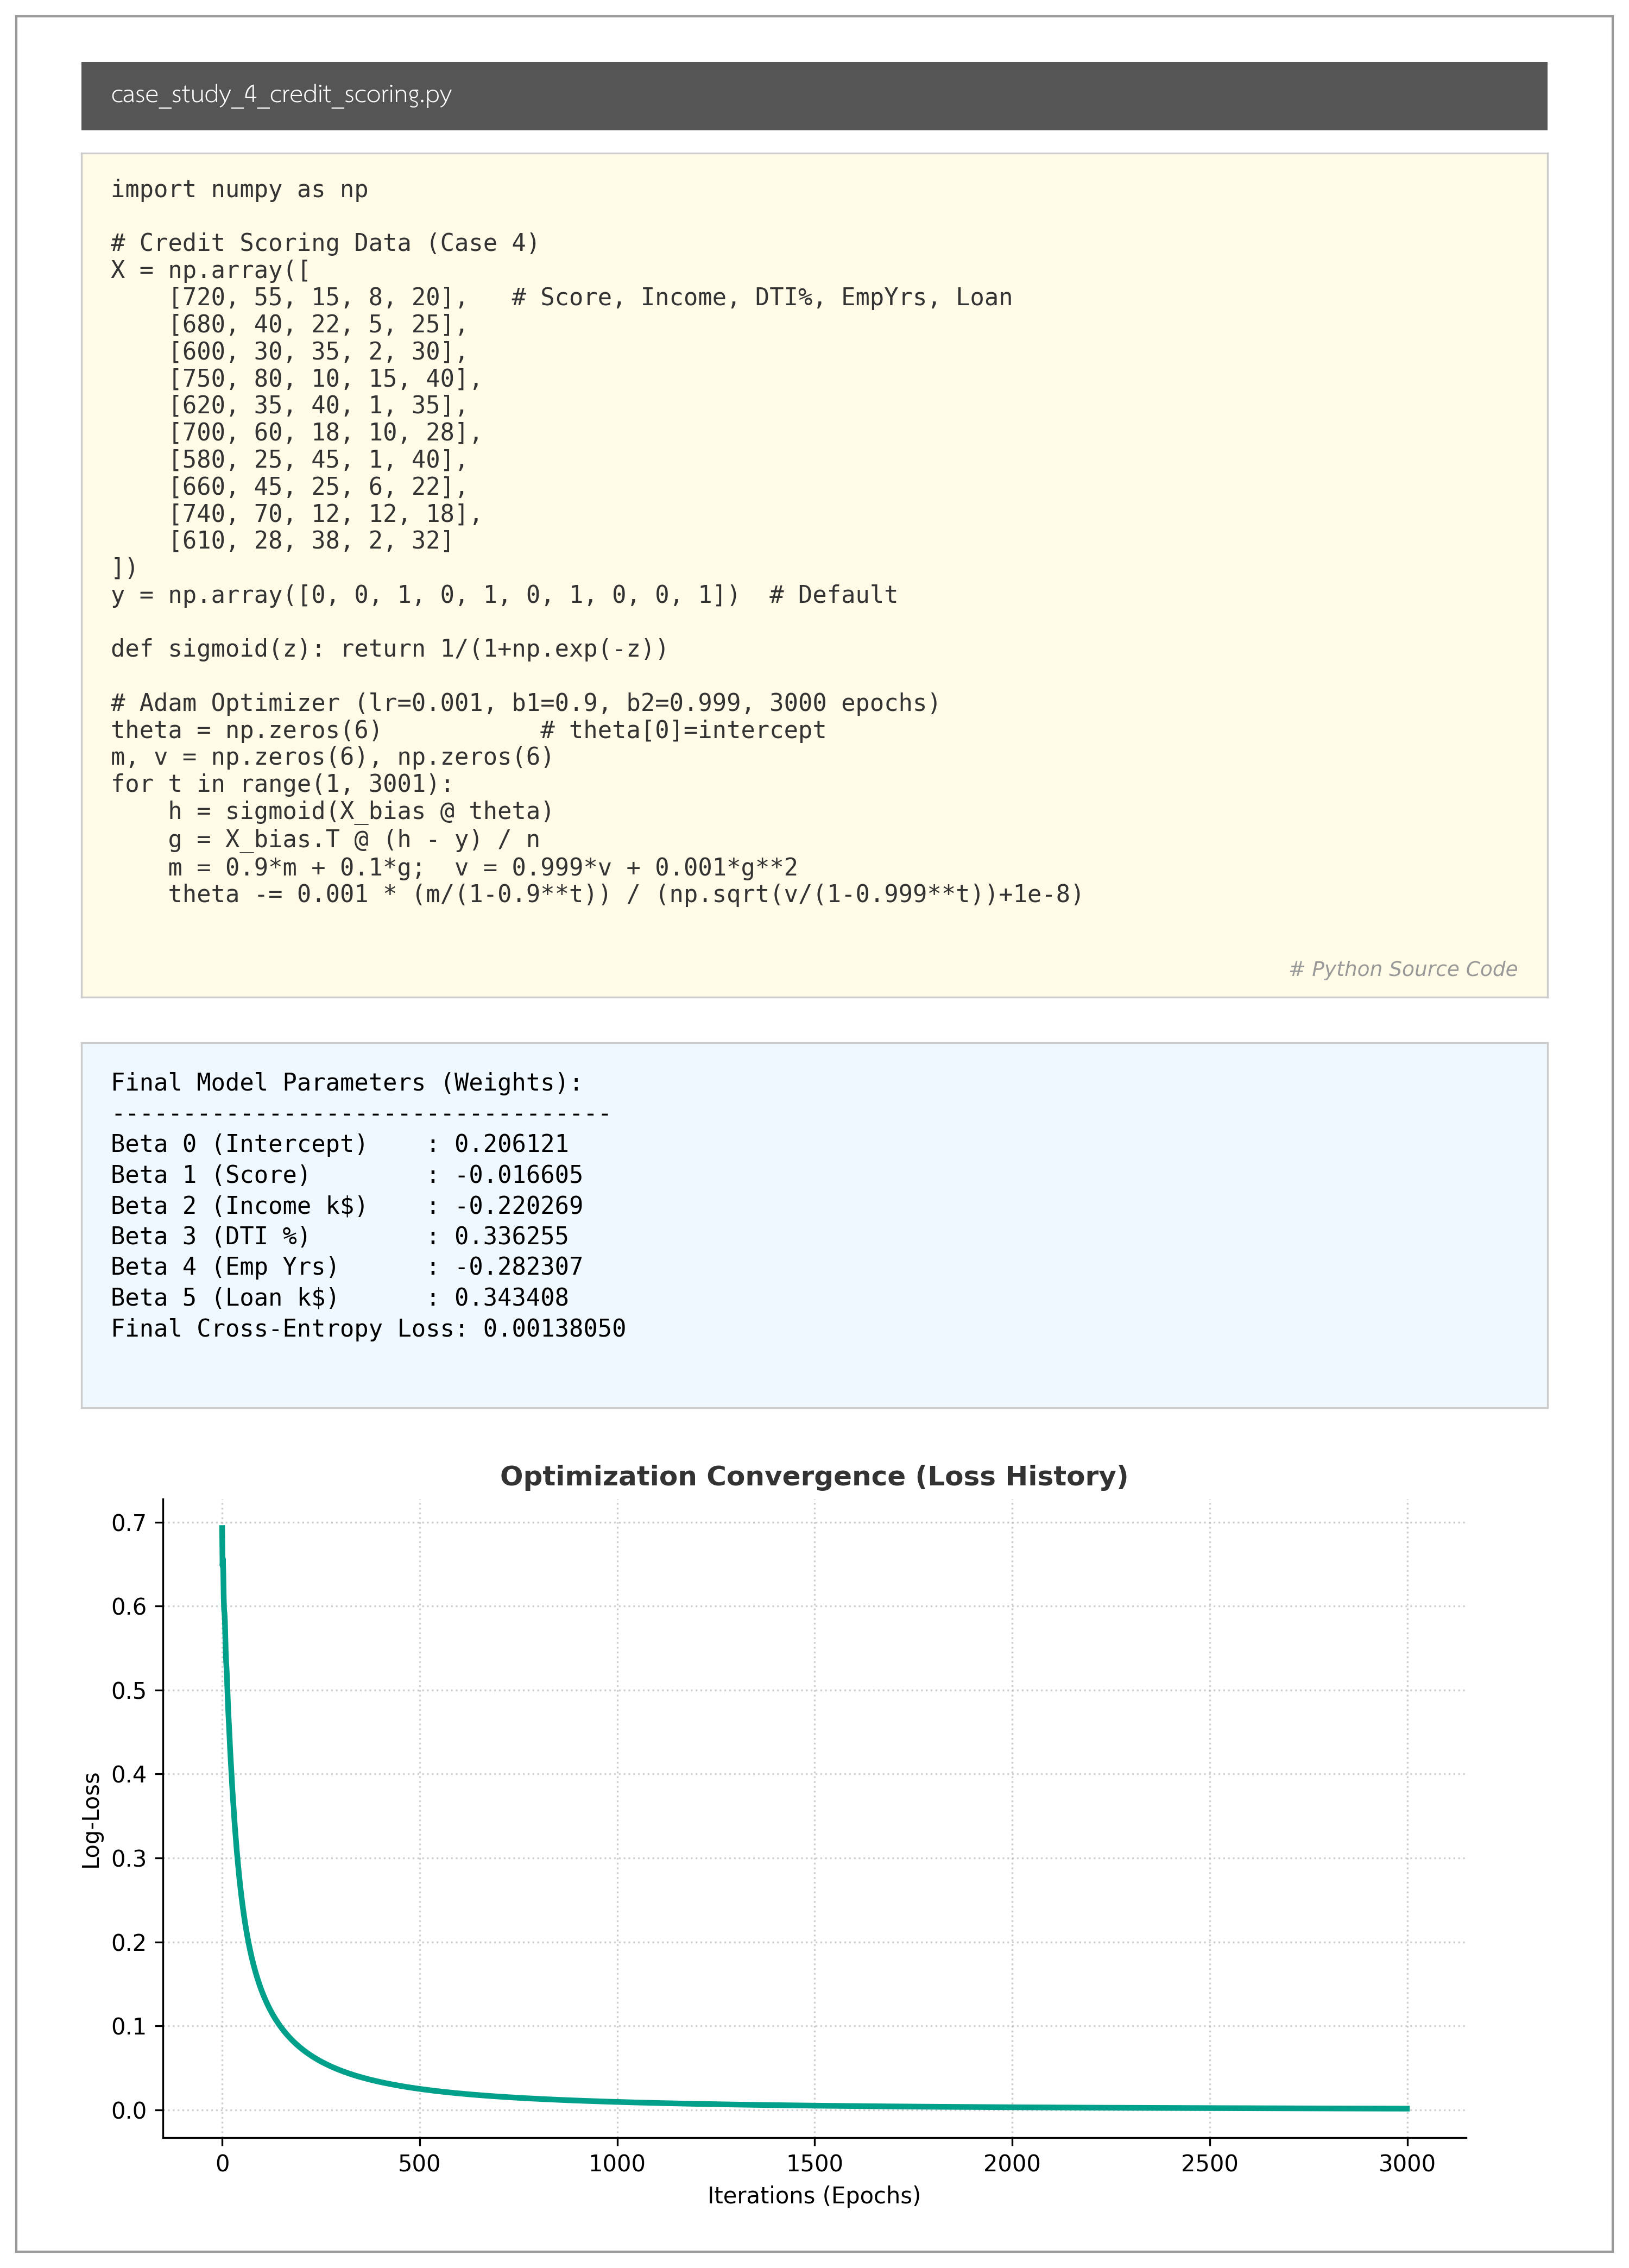
\includegraphics[width=1\textwidth]{CH3_case4_adam_results.png}
	\caption{Python Code และผลลัพธ์การประมาณค่าพารามิเตอร์ของกรณีศึกษาที่ 4 ด้วยอัลกอริทึม Adam พร้อมกราฟแสดงการลู่เข้าของค่าความสูญเสีย (Loss Curve)}
	\label{fig:case4_results}
\end{figure}






%######################################

\section{การถดถอยแบบ Regularization}
การถดถอยแบบ Regularization เป็นเทคนิคที่ใช้เพื่อป้องกันปัญหา Overfitting ในกรณีที่ตัวแบบมีความซับซ้อนมากเกินไปหรือมีตัวแปรอิสระจำนวนมาก โดยการเพิ่มข้อจำกัด (Penalty Term) เข้าไปในฟังก์ชันความสูญเสีย (Loss Function) เพื่อจำกัดไม่ให้ค่าสัมประสิทธิ์มีขนาดใหญ่เกินไป

\subsection{Ridge Regression (L2 Regularization)}
Ridge Regression หรือ L2 Regularization เป็นวิธีการที่เพิ่มข้อจำกัดในรูปของผลรวมกำลังสองของสัมประสิทธิ์ทั้งหมด โดยมีฟังก์ชันวัตถุประสงค์ดังนี้

\[
\hat{\boldsymbol{\beta}}^{\text{Ridge}} = \arg\min_{\boldsymbol{\beta}} \left\{ \sum_{i=1}^{n}(y_i - \mathbf{x}_i^T\boldsymbol{\beta})^2 + \lambda \sum_{j=1}^{k}\beta_j^2 \right\}
\]

โดยที่ $\lambda \geq 0$ คือค่า Hyperparameter ที่ควบคุมความเข้มของการ Regularize

\begin{exmp}
\label{exmp:ridge_regression_example}
พิจารณาตัวอย่างการประมาณค่าสัมประสิทธิ์ด้วย Ridge Regression จากข้อมูล 3 ชุด โดยมี $n=3$, $k=2$ และ $\lambda = 0.5$ กำหนดให้ค่าสังเกต $(y_1, y_2, y_3) = (3, 2, 4)$ และค่าตัวแปรอิสระ $\mathbf{X} = \begin{bmatrix} 1 & 2 \\ 1 & 3 \\ 1 & 4 \end{bmatrix}$

สมมติได้ค่าประมาณจาก OLS คือ $\hat{\beta}_0 = 1.0$ และ $\hat{\beta}_1 = 0.8$ เมื่อใช้ Ridge ด้วย $\lambda = 0.5$ จะได้

\[
\hat{\beta}_0^{\text{Ridge}} = 1.0, \qquad \hat{\beta}_1^{\text{Ridge}} = \frac{0.8}{1 + 0.5} \approx 0.53
\]

จะเห็นได้ว่าค่า $\hat{\beta}_1$ ถูกลดขนาดลง (Shrinkage) จาก 0.8 เป็น 0.53 ทำให้ตัวแบบมีความเสถียรมากขึ้น
\end{exmp}

\subsection{Lasso Regression (L1 Regularization)}
Lasso Regression หรือ L1 Regularization เป็นวิธีการที่เพิ่มข้อจำกัดในรูปของผลรวมค่าสัมบูรณ์ของสัมประสิทธิ์ ซึ่งมีคุณสมบัติพิเศษในการทำ Feature Selection อัตโนมัติโดยการตัดค่าสัมประสิทธิ์บางตัวให้เป็นศูนย์

\[
\hat{\boldsymbol{\beta}}^{\text{Lasso}} = \arg\min_{\boldsymbol{\beta}} \left\{ \sum_{i=1}^{n}(y_i - \mathbf{x}_i^T\boldsymbol{\beta})^2 + \lambda \sum_{j=1}^{k}|\beta_j| \right\}
\]

\begin{exmp}
\label{exmp:lasso_regression_example}
พิจารณาเปรียบเทียบผลของ Ridge และ Lasso บนข้อมูลชุดเดียวกัน สมมติได้ค่าสัมประสิทธิ์จาก OLS คือ $\hat{\boldsymbol{\beta}} = (0.5, 1.2, -0.8, 0.3)^T$ เมื่อใช้ $\lambda = 1.0$

สำหรับ Ridge ($\lambda \sum\beta_j^2$): $\hat{\beta}^{\text{Ridge}} = (0.33, 0.80, -0.53, 0.20)^T$

สำหรับ Lasso ($\lambda \sum|\beta_j|$): $\hat{\beta}^{\text{Lasso}} = (0.0, 0.7, -0.3, 0.0)^T$

จะเห็นได้ว่า Lasso ทำให้ $\beta_1$ และ $\beta_4$ ถูกตัดออกเป็นศูนย์ ซึ่งแสดงคุณสมบัติ Feature Selection ของ Lasso
\end{exmp}

\subsection{Elastic Net Regression}
Elastic Net ผสมผสานข้อดีของทั้ง Ridge และ Lasso โดยใช้ Penalty ทั้ง L1 และ L2 พร้อมกัน

\[
\hat{\boldsymbol{\beta}}^{\text{Elastic}} = \arg\min_{\boldsymbol{\beta}} \left\{ \sum_{i=1}^{n}(y_i - \mathbf{x}_i^T\boldsymbol{\beta})^2 + \lambda_1 \sum_{j=1}^{k}|\beta_j| + \lambda_2 \sum_{j=1}^{k}\beta_j^2 \right\}
\]

\subsection{การเกำหนดค่า Hyperparameter}
การเลือกค่า $\lambda$ ที่เหมาะสมเป็นสิ่งสำคัญสำหรับทุกวิธี Regularization โดยทั่วไปใช้วิธี Cross-Validation เพื่อหาค่า $\lambda$ ที่ให้ค่า Validation Error ต่ำที่สุด


%\section*{แบบฝึกหัด (Assignment)}
%
%\subsection*{ส่วนที่ 1: แบบเติมคำ (Fill-in-the-blank)}
%
%\noindent จงเติมคำลงในช่องว่างให้ถูกต้องสมบูรณ์ตามหลักการของการถดถอยโลจิสติคและอัลกอริทึม Adam
%
%\begin{enumerate}
%
%	\item ฟังก์ชันที่ทำหน้าที่แปลงค่าความน่าจะเป็น ($p$) ให้อยู่ในรูปของ Log-Odds มีชื่อเรียกว่าฟังก์ชัน \textbf{.......................} และฟังก์ชันผกผัน (Inverse) ของมันซึ่งแปลงจาก Log-Odds กลับเป็นความน่าจะเป็นเรียกว่าฟังก์ชัน \textbf{.......................}
%	
%	\item ในการถดถอยโลจิสติค เราเลือกใช้วิธีการ \textbf{.............................................} (MLE) ในการประมาณค่าพารามิเตอร์ แทนวิธีกำลังสองน้อยที่สุด (OLS) เนื่องจากตัวแปรตามเป็นค่า \textbf{.......................} (Binary)
%	
%	\item เวกเตอร์ของอนุพันธ์อันดับหนึ่งของฟังก์ชัน Log-Likelihood เมื่อเทียบกับพารามิเตอร์ $\beta$ มีชื่อเรียกเฉพาะว่า \textbf{.......................} และสำหรับการถดถอยโลจิสติค มีรูปแบบเมทริกซ์คือ $\mathbf{g} = \mathbf{X}^T(\textbf{\underline{\hspace{2cm}}})$
%	
%	\item เมทริกซ์เฮสเซียน (Hessian Matrix) ของฟังก์ชัน Log-Likelihood ในการถดถอยโลจิสติค มีคุณสมบัติเป็น \textbf{.......................} ซึ่งรับประกันว่าจุดที่หาได้เป็นจุด \textbf{.......................} (Unique Global Maximum)
%	
%	\item อัลกอริทึมนิวตัน-ราฟสันมีอัตราการลู่เข้าในระดับ \textbf{.......................} แต่ต้องแลกมาด้วยต้นทุนการคำนวณที่สูงเพราะต้องหาค่าผกผัน (Inverse) ของ \textbf{.......................} ในแต่ละรอบ
%	
%	\item อัลกอริทึม Adam ย่อมาจาก \textbf{.............................................} ซึ่งเป็นวิธีการผสมผสานแนวคิดของ \textbf{.......................} และ \textbf{.......................} เข้าด้วยกัน
%	
%	\item ค่าเฉลี่ยเคลื่อนที่แบบเอ็กซ์โพเนนเชียล (EMA) ของเกรเดียนต์อันดับหนึ่งใน Adam เรียกว่า \textbf{.......................} ($m_t$) ส่วน EMA ของกำลังสองของเกรเดียนต์เรียกว่า \textbf{.......................} ($v_t$)
%	
%	\item ค่าพารามิเตอร์ $\beta_1 = 0.9$ และ $\beta_2 = 0.999$ ในอัลกอริทึม Adam เป็นอัตราการลดทอน (Decay Rate) ของ \textbf{.......................} และ \textbf{.......................} ตามลำดับ
%	
%	\item เหตุผลที่ต้องทำ Bias Correction ใน Adam คือ ค่าเริ่มต้น $m_0 = 0$ และ $v_0 = 0$ ทำให้ตัวประมาณค่ามีค่า \textbf{.......................} เกินจริงในช่วงรอบแรกๆ สูตร Bias Correction ของ First Moment คือ $\hat{m}_t = \dfrac{m_t}{1 - \beta_1^{\textbf{\underline{\hspace{0.5cm}}}}}$
%	
%	\item ข้อดีสำคัญของ Adaptive Learning Rate ใน Adam เมื่อเทียบกับ SGD คือ Adam ปรับขนาดก้าวให้ \textbf{.......................} สำหรับพารามิเตอร์แต่ละตัว โดยพารามิเตอร์ที่มีเกรเดียนต์ใหญ่จะได้รับก้าวที่ \textbf{.......................} โดยอัตโนมัติ
%	
%	\item ค่าคงที่ $\epsilon$ (เช่น $10^{-8}$) ในสูตร Adam ถูกเพิ่มเข้าไปในตัวหารเพื่อป้องกัน \textbf{.......................} และทำให้การคำนวณมีเสถียรภาพทางตัวเลข
%	
%	\item อัลกอริทึม Adam มีอัตราการลู่เข้าแบบ \textbf{.......................} ซึ่งช้ากว่า Newton-Raphson แต่มีข้อได้เปรียบด้านความสามารถรับมือกับ \textbf{.......................} และข้อมูลขนาดใหญ่
%	
%	\item ในกรณีที่ข้อมูลมีขนาดใหญ่มาก อัลกอริทึม Adam ใช้แนวคิดของ \textbf{.......................} (Mini-batch) ในการคำนวณเกรเดียนต์ เพื่อลดภาระการคำนวณในแต่ละรอบ
%
%\end{enumerate}
%
%\subsection*{ส่วนที่ 2: แสดงวิธีทำ (Calculations)}
%
%\textbf{ข้อ 1: (การคำนวณ Odds และ Logit)} หากกำหนดให้ความน่าจะเป็นที่ผู้ป่วยจะหายจากโรค ($p$) เท่ากับ 0.8 จงคำนวณหาค่า Odds ของการหายจากโรค และค่า Logit($p$) พร้อมแสดงขั้นตอน
%
%
%\textbf{ข้อ 2: (การสร้างฟังก์ชัน Likelihood)} กำหนดข้อมูลสังเกตการณ์ 1 ชุด คือ $(y_1, x_1) = (1, 2)$ โดยใช้แบบจำลอง $\text{logit}(p_1) = \beta_1 x_1$ จงเขียนฟังก์ชัน Likelihood $L(\beta_1)$ ในรูปของ $\beta_1$
%
%
%\textbf{ข้อ 3: (การคำนวณรอบการวนซ้ำของนิวตัน-ราฟสัน)} ในรอบที่ $t$ ได้ค่า Score function $S(\beta^{(t)}) = 0.5$ และ Hessian $H(\beta^{(t)}) = -2.0$ หากเริ่มต้นด้วย $\beta^{(t)} = 1.0$ จงคำนวณ $\beta^{(t+1)}$ โดยใช้อัลกอริทึมนิวตัน-ราฟสัน
%
%
%\textbf{ข้อ 4: (Bias Correction)} กำหนดให้ในรอบที่ $t = 3$ ของ Adam มีค่า $m_3 = -1.026$ และ $\beta_1 = 0.9$ จงคำนวณ $\hat{m}_3$ และอธิบายว่าทำไม $|\hat{m}_3| > |m_3|$ ในช่วงรอบแรกๆ
%
%
%\textbf{ข้อ 5: (Adam รอบแรก)} กำหนดค่า $\beta^{(0)} = 0.5$, $\alpha = 0.1$, $\beta_1 = 0.9$, $\beta_2 = 0.999$, $\epsilon = 10^{-8}$, $m_0 = 0$, $v_0 = 0$ และเกรเดียนต์รอบแรก $g_1 = 3.0$ จงคำนวณทีละขั้น: $m_1$, $v_1$, $\hat{m}_1$, $\hat{v}_1$ และ $\beta^{(1)}$
%
%
%\textbf{ข้อ 6: (การคำนวณเกรเดียนต์)} กำหนดข้อมูลสังเกตการณ์ 3 ชุด และแบบจำลองมีตัวแปร $(\beta_0, \beta_1)$:
%\begin{center}\small
%\begin{tabular}{|c|c|c|c|}\hline
%$i$ & $x_i$ & $y_i$ & $p_i$ \\ \hline
%1 & 1 & 0 & 0.5 \\
%2 & 2 & 1 & 0.5 \\
%3 & 3 & 1 & 0.5 \\ \hline
%\end{tabular}\end{center}
%จงคำนวณ $g_{\beta_0}$ และ $g_{\beta_1}$ โดยใช้ $\mathbf{g} = \mathbf{X}^T(\mathbf{p} - \mathbf{y})$
%
%
%\textbf{ข้อ 7: (การทำนายจากโมเดลที่ฝึกด้วย Adam)} หลังจากฝึกด้วย Adam ได้พารามิเตอร์ $\hat{\boldsymbol{\beta}} = [-2.5, 0.04, 0.08, -0.03]^T$ สำหรับตัวแปร (Intercept, Age, Glucose, BMI) ตามลำดับ จงทำนายความน่าจะเป็นการเป็นโรคเบาหวานของผู้ป่วยที่มี Age = 50, Glucose = 120, BMI = 28
%
%
%%######################################
%\newpage
%\section{เฉลยแบบฝึกหัด (Solutions)}
%
%\subsection{ส่วนที่ 1: แบบเติมคำ}
%\begin{enumerate}
%	\item Logit Function (แปลง $p$ ไปเป็น Log-Odds) และ Sigmoid Function / Logistic Function (แปลงกลับ)
%	\item Maximum Likelihood Estimation (MLE) / ไม่ต่อเนื่อง (Discrete)
%	\item Score Function; $\mathbf{X}^T(\mathbf{p} - \mathbf{y})$
%	\item Negative Definite; สูงสุดสัมบูรณ์เพียงจุดเดียว (Unique Global Maximum)
%	\item Quadratic Convergence (การลู่เข้าลำดับสอง); เมทริกซ์เฮสเซียน (Hessian Matrix)
%	\item Adaptive Moment Estimation; Momentum (First Moment) และ Adaptive Learning Rate (RMSProp)
%	\item First Moment / Momentum; Second Moment
%	\item First Moment ($m_t$); Second Moment ($v_t$)
%	\item ต่ำเกินจริง (Underestimated); $t$ (จำนวนรอบการวนซ้ำ)
%	\item แตกต่างกันสำหรับแต่ละพารามิเตอร์ (Individualized); เล็กลง (Smaller)
%	\item การหารด้วยศูนย์ (Division by Zero) หรือค่าไม่เสถียรทางตัวเลข (Numerical Instability)
%	\item Linear Convergence; Noisy Gradient (เกรเดียนต์มีสัญญาณรบกวน)
%	\item Stochastic Gradient Descent / Mini-batch Gradient Descent
%\end{enumerate}
%
%\subsection{ส่วนที่ 2: แสดงวิธีทำ}
%
%\textbf{เฉลยข้อ 1: การคำนวณ Odds และ Logit}
%\begin{itemize}
%	\item $\text{Odds} = \dfrac{p}{1-p} = \dfrac{0.8}{0.2} = 4$
%	\item $\text{Logit}(0.8) = \ln(4) \approx 1.386$
%	\item \textbf{สรุป:} Odds ของการหายจากโรคคือ 4 และค่า Logit คือ 1.386
%\end{itemize}
%
%\textbf{เฉลยข้อ 2: การสร้างฟังก์ชัน Likelihood}
%\begin{itemize}
%	\item จาก $y_1 = 1$: $L(\beta_1) = P(Y=1|x_1) = \sigma(\beta_1 x_1) = \dfrac{1}{1 + e^{-\beta_1(2)}} = \dfrac{1}{1 + e^{-2\beta_1}}$
%\end{itemize}
%
%\textbf{เฉลยข้อ 3: การวนซ้ำนิวตัน-ราฟสัน}
%\begin{itemize}
%	\item Update Rule: $\beta^{(t+1)} = \beta^{(t)} - \dfrac{S(\beta^{(t)})}{H(\beta^{(t)})} = 1.0 - \dfrac{0.5}{-2.0} = 1.0 + 0.25 = 1.25$
%\end{itemize}
%
%\textbf{เฉลยข้อ 4: Bias Correction}
%\begin{itemize}
%	\item $\hat{m}_3 = \dfrac{-1.026}{1 - 0.9^3} = \dfrac{-1.026}{0.271} \approx -3.786$
%	\item $|\hat{m}_3| > |m_3|$ เพราะ $m_t$ เริ่มจาก 0 ทำให้ค่าต่ำกว่าความเป็นจริง การหารด้วย $(1 - \beta_1^t) < 1$ จึงขยายค่ากลับ
%\end{itemize}
%
%\textbf{เฉลยข้อ 5: Adam รอบแรก}
%\begin{itemize}
%	\item $m_1 = 0.9(0) + 0.1(3.0) = 0.3$;  $v_1 = 0.999(0) + 0.001(9.0) = 0.009$
%	\item $\hat{m}_1 = 0.3/(1-0.9) = 3.0$;  $\hat{v}_1 = 0.009/(1-0.999) = 9.0$
%	\item $\beta^{(1)} = 0.5 - \dfrac{0.1}{\sqrt{9.0}+10^{-8}}(3.0) = 0.5 - 0.1 = 0.4$
%\end{itemize}
%
%\textbf{เฉลยข้อ 6: การคำนวณเกรเดียนต์}
%\begin{itemize}
%	\item $g_{\beta_0} = (1)(0.5) + (1)(-0.5) + (1)(-0.5) = -0.5$
%	\item $g_{\beta_1} = (1)(0.5) + (2)(-0.5) + (3)(-0.5) = -2.0$
%	\item $\mathbf{g} = [-0.5, -2.0]^T$ — ทิศทางลบบ่งชี้ว่า Adam จะเพิ่มค่า $\beta$ เพื่อลดค่าสูญเสีย
%\end{itemize}
%
%\textbf{เฉลยข้อ 7: การทำนาย}
%\begin{itemize}
%	\item $\hat{y} = -2.5 + 0.04(50) + 0.08(120) - 0.03(28) = -2.5 + 2.0 + 9.6 - 0.84 = 8.26$
%	\item $P(Y=1) = \dfrac{1}{1 + e^{-8.26}} \approx 0.9997 \approx 99.97\%$
%\end{itemize}
%
%
%
%
%
%
%\begin{enumerate}
%
%	\item เหตุผลที่ต้องทำ Bias Correction ใน Adam คือ ค่าเริ่มต้น $m_0 = 0$ ทำให้ตัวประมาณค่ามีค่า \textbf{.........................................................................} เกินจริงในรอบแรกๆ
%
%	\item สูตร Bias Correction ของ First Moment คือ $\hat{m}_t = m_t / (1 - \beta_1^t)$ โดยที่ $t$ หมายถึง \textbf{.........................................................................}
%
%	\item ในบริบทของการถดถอยโลจิสติค เกรเดียนต์ที่ใช้ใน Adam คือ $\mathbf{g} = \mathbf{X}^T(\mathbf{p} - \mathbf{y})$ ซึ่งเป็นลบของ \textbf{.........................................................................} ที่ได้จากวิธี MLE
%
%	\item ข้อได้เปรียบสำคัญของ Adaptive Learning Rate ใน Adam เมื่อเทียบกับ SGD ธรรมดา คือ Adam สามารถปรับอัตราการเรียนรู้ให้ \textbf{.........................................................................} สำหรับพารามิเตอร์แต่ละตัวโดยอัตโนมัติ
%
%	\item เมื่อ $\sqrt{\hat{v}_t}$ มีขนาดใหญ่ ขนาดก้าวของการอัปเดตพารามิเตอร์จะมีขนาด \textbf{.........................................................................} ซึ่งช่วยป้องกันการกระโดดข้ามจุดเหมาะสมที่สุด
%
%	\item ค่าคงที่ $\epsilon$ (เช่น $10^{-8}$) ในตัวหาร $\sqrt{\hat{v}_t} + \epsilon$ ของ Adam ถูกเพิ่มเข้ามาเพื่อป้องกัน \textbf{.........................................................................}
%
%	\item อัลกอริทึม Adam มีอัตราการลู่เข้า (Convergence Rate) แบบ \textbf{.........................................................................} ซึ่งช้ากว่า Quadratic ของนิวตัน-ราฟสัน แต่เหมาะกับข้อมูลขนาดใหญ่กว่า
%\end{enumerate}
%
%\subsection*{ส่วนที่ 2: แสดงวิธีทำ (Calculations)}
%
%\textbf{ข้อ 1: (Bias Correction)} กำหนดให้ในรอบที่ $t = 3$ ของ Adam มีค่า $m_3 = -1.026$ และ $\beta_1 = 0.9$ จงคำนวณ $\hat{m}_3$ และอธิบายว่าทำไม $|\hat{m}_3| > |m_3|$ ในช่วงรอบแรกๆ
%
%
%\textbf{ข้อ 2: (Adam รอบแรก)} กำหนดค่าเริ่มต้น $\beta^{(0)} = 0.5$, $\alpha = 0.1$, $\beta_1 = 0.9$, $\beta_2 = 0.999$, $\epsilon = 10^{-8}$, $m_0 = 0$, $v_0 = 0$ และเกรเดียนต์รอบแรก $g_1 = 3.0$ จงคำนวณ $m_1$, $v_1$, $\hat{m}_1$, $\hat{v}_1$ และ $\beta^{(1)}$
%
%
%\textbf{ข้อ 3: (การคำนวณเกรเดียนต์สำหรับ Adam)} กำหนดข้อมูลสังเกตการณ์ 3 ชุด ดังนี้
%
%\begin{center}\small
%\begin{tabular}{|c|c|c|c|}\hline
%$i$ & $x_i$ & $y_i$ & $p_i$ \\ \hline
%1 & 1 & 0 & 0.5 \\
%2 & 2 & 1 & 0.5 \\
%3 & 3 & 1 & 0.5 \\ \hline
%\end{tabular}\end{center}
%\noindent โดยแบบจำลองมีตัวแปร $(\beta_0, \beta_1)$ จงคำนวณ $g_{\beta_0}$ และ $g_{\beta_1}$ โดยใช้ $\mathbf{g} = \mathbf{X}^T(\mathbf{p} - \mathbf{y})$
%
%
%\textbf{ข้อ 4: (Adam กับ SGD)} กำหนดเกรเดียนต์ $g = 3.0$ และพารามิเตอร์ปัจจุบัน $\beta = 0.5$
%\begin{enumerate}[label=(\alph*)]
%    \item หากใช้ SGD ที่ $\alpha = 0.1$ จงคำนวณ $\beta_{\text{new}}$
%    \item หากใช้ Adam ที่ $t=1$, $\alpha = 0.1$, $m_0 = 0$, $v_0 = 0$, $\beta_1 = 0.9$, $\beta_2 = 0.999$ จงคำนวณ $\beta_{\text{new}}$
%    \item จงอภิปรายว่าทำไมขนาดก้าวของ Adam แตกต่างจาก SGD
%\end{enumerate}
%
%
%\textbf{ข้อ 5: (การทำนายจากโมเดลที่ฝึกด้วย Adam)} หลังจากฝึกด้วย Adam ได้พารามิเตอร์ $\hat{\boldsymbol{\beta}} = [-2.5, 0.04, 0.08, -0.03]^T$ สำหรับตัวแปร (Intercept, Age, Glucose, BMI) ตามลำดับ จงทำนายความน่าจะเป็นการเป็นโรคเบาหวานของผู้ป่วยที่มี Age = 50, Glucose = 120, BMI = 28 โดยแสดงขั้นตอนการคำนวณ
%
%\newpage
%
%\section{เฉลยแบบฝึกหัด (Solutions)}

%\subsection{ส่วนที่ 1: แบบเติมคำ}
%\begin{enumerate}
%	\item Adaptive Moment Estimation (การประมาณค่าโมเมนต์แบบปรับตัว)
%	\item Momentum / First Moment ($m_t$)
%	\item Second Moment Estimate / EMA ของ Gradient กำลังสอง ($v_t$)
%	\item ต่ำเกินจริง (Underestimated)
%	\item จำนวนรอบการวนซ้ำ (Iteration Number)
%	\item Score Function $\mathbf{S}(\boldsymbol{\beta}) = \mathbf{X}^T(\mathbf{y} - \mathbf{p})$
%	\item แตกต่างกัน (Individualized / Different) สำหรับพารามิเตอร์แต่ละตัว
%	\item เล็กลง (Smaller) -- ขนาดก้าวถูกหดลงโดยอัตโนมัติ
%	\item การหารด้วยศูนย์ (Division by Zero) หรือค่าไม่เสถียรทางตัวเลข
%	\item เชิงเส้น (Linear Convergence)
%\end{enumerate}
%
%\subsection{ส่วนที่ 2: แสดงวิธีทำ}
%
%\textbf{เฉลยข้อ 1: Bias Correction}
%\begin{itemize}
%	\item $\hat{m}_3 = \dfrac{-1.026}{1 - 0.9^3} = \dfrac{-1.026}{0.271} \approx -3.786$
%	\item $|\hat{m}_3| > |m_3|$ เนื่องจากในรอบแรก $m_t$ ยังไม่สะสมข้อมูลพอ (เริ่มต้นจาก 0) การหารด้วย $(1 - \beta_1^t) < 1$ จึงขยายค่ากลับให้สะท้อนเกรเดียนต์ที่แท้จริง
%\end{itemize}
%
%\textbf{เฉลยข้อ 2: Adam รอบแรก}
%\begin{itemize}
%	\item $m_1 = 0.9(0) + 0.1(3.0) = 0.3$
%	\item $v_1 = 0.999(0) + 0.001(3.0)^2 = 0.009$
%	\item $\hat{m}_1 = 0.3/(1-0.9) = 3.0$
%	\item $\hat{v}_1 = 0.009/(1-0.999) = 9.0$
%	\item $\beta^{(1)} = 0.5 - \dfrac{0.1}{\sqrt{9.0}+10^{-8}}(3.0) = 0.5 - \dfrac{0.1}{3.0}(3.0) = 0.5 - 0.1 = 0.4$
%\end{itemize}
%
%\textbf{เฉลยข้อ 3: การคำนวณเกรเดียนต์}
%\begin{itemize}
%	\item $g_{\beta_0} = (1)(0.5-0) + (1)(0.5-1) + (1)(0.5-1) = 0.5 - 0.5 - 0.5 = -0.5$
%	\item $g_{\beta_1} = (1)(0.5-0) + (2)(0.5-1) + (3)(0.5-1) = 0.5 - 1.0 - 1.5 = -2.0$
%	\item \textbf{สรุป:} $\mathbf{g} = [-0.5, -2.0]^T$ ทิศทางลบบ่งชี้ว่า Adam จะเพิ่มค่า $\beta$ เพื่อลดค่าสูญเสีย
%\end{itemize}
%
%\textbf{เฉลยข้อ 4: Adam กับ SGD}
%\begin{enumerate}[label=(\alph*)]
%	\item SGD: $\beta_{\text{new}} = 0.5 - (0.1)(3.0) = 0.2$
%	\item Adam ($t=1$): จากข้อ 2 ได้ $\beta_{\text{new}} = 0.4$
%	\item ขนาดก้าวของ Adam ถูกหารด้วย $\sqrt{\hat{v}_t}$ สะท้อนขนาดเกรเดียนต์ ทำให้ขนาดก้าวใกล้เคียง $\alpha$ เสมอ ต่างจาก SGD ที่ขนาดก้าวผันตาม $g$ โดยตรง
%\end{enumerate}
%
%\textbf{เฉลยข้อ 5: การทำนาย}
%\begin{itemize}
%	\item $\hat{y} = -2.5 + 0.04(50) + 0.08(120) + (-0.03)(28) = -2.5 + 2.0 + 9.6 - 0.84 = 8.26$
%	\item $P(Y=1) = \dfrac{1}{1 + e^{-8.26}} \approx 0.9997$
%	\item \textbf{สรุป:} ผู้ป่วยรายนี้มีความน่าจะเป็นการเป็นโรคเบาหวานประมาณ 99.97\%
%\end{itemize}
%
